%% LyX 2.4.3 created this file.  For more info, see https://www.lyx.org/.
%% Do not edit unless you really know what you are doing.
\documentclass[journal,article,submit,pdftex,moreauthors]{Definitions/mdpi}
\usepackage{textcomp}
\usepackage[utf8]{inputenc}
\usepackage{array}
\usepackage{cprotect}
\usepackage{float}
\usepackage{url}
\usepackage{bm}
\usepackage{multirow}
\usepackage{varwidth}
\usepackage{amsmath}
\usepackage{graphicx}

\makeatletter

%%%%%%%%%%%%%%%%%%%%%%%%%%%%%% LyX specific LaTeX commands.

\Title{Parallel Balanced Grey Wolf Optimizer: A Cooperative Parallel Approach
for Large-Scale Optimization Problems}

\Author{Glykeria Kyrou$^{1}$, Konstantinos G. Barkas $^{2}$, Vasileios Charilogis$^{3}$
and Ioannis G. Tsoulos$^{4}$ }


\address{$^{1}$\quad{}Department of Informatics and Telecommunications,
University of Ioannina, 47150 Kostaki Artas, Greece; g.kyrou@uoi.gr\\
$^{2}$\quad{}Department of Informatics and Telecommunications, University
of Ioannina, 47150 Kostaki Artas, Greece; kbarkas@uoi.gr\\
$^{3}$\quad{}Department of Informatics and Telecommunications, University
of Ioannina, 47150 Kostaki Artas, Greece; v.charilog@uoi.gr \\
$^{4}$\quad{}Department of Informatics and Telecommunications, University
of Ioannina, 47150 Kostaki Artas, Greece; itsoulos@uoi.gr \\
}


\corres{Correspondence: g.kyrou@uoi.gr}


\abstract{In recent years, large-scale optimization problems have become increasingly
common in various fields, such as machine learning and data analysis,
generating increased references to both computational cost and accurate
solutions. The Grey Wolf Optimizer (GWO) is an efficient collective
intelligence algorithm, however its performance may be limited when
high-permissive problems are allowed or in environments with strong
multimodal landscapes. In this paper, we propose the Parallel Balanced
Grey Wolf Optimizer (ParallelBGWO), a parallel extension of GWO that
aims to improve the balance between exploration and exploitation of
the search space. The proposed algorithm divides the total population
into multiple subpopulations, which cooperate through information
exchange. This cooperation reduces the probability of premature convergence
and enhances the global search. The parallel implementation exploits
modern multi-core computing architectures, achieving a significant
reduction in execution time, while at the same time maintaining or
improving the quality of the final solutions. Experimental evaluations
on high-dimensional benchmark functions show that ParallelBGWO exhibits
faster convergence and reduced number of objective function evaluations
compared to the classical version of GWO and other prominent methods.
The results highlight ParallelBGWO as an efficient approach for demanding
global optimization problems.}


\keyword{Global optimization; GWO algorithm; Evolutionary techniques; Stochastic
methods; Large-scale problems}

\newcommand*\LyXZeroWidthSpace{\hspace{0pt}}
%% Because html converters don't know tabularnewline
\providecommand{\tabularnewline}{\\}
%% Variable width box for table cells
\newenvironment{cellvarwidth}[1][t]
    {\begin{varwidth}[#1]{\linewidth}}
    {\@finalstrut\@arstrutbox\end{varwidth}}
%% A simple dot to overcome graphicx limitations
\newcommand{\lyxdot}{.}

\floatstyle{ruled}
\newfloat{algorithm}{tbp}{loa}
\providecommand{\algorithmname}{Algorithm}
\floatname{algorithm}{\protect\algorithmname}

%%%%%%%%%%%%%%%%%%%%%%%%%%%%%% User specified LaTeX commands.
%  LaTeX support: latex@mdpi.com 
%  For support, please attach all files needed for compiling as well as the log file, and specify your operating system, LaTeX version, and LaTeX editor.

%=================================================================
%\documentclass[preprints,article,submit,pdftex,moreauthors]{Definitions/mdpi} 
% For posting an early version of this manuscript as a preprint, you may use "preprints" as the journal. Changing "submit" to "accept" before posting will remove line numbers.

% Below journals will use APA reference format:
% admsci, aieduc, behavsci, businesses, econometrics, economies, education, ejihpe, famsci, games, humans, ijcs, ijfs, jintelligence, journalmedia, jrfm, jsam, languages, peacestud, psycholint, publications, tourismhosp, youth

% Below journals will use Chicago reference format:
% arts, genealogy, histories, humanities, laws, literature, religions, risks, socsci

%--------------------
% Class Options:
%--------------------
%----------
% journal
%----------
% Choose between the following MDPI journals:
% accountaudit, acoustics, actuators, addictions, adhesives, admsci, adolescents, aerobiology, aerospace, agriculture, agriengineering, agrochemicals, agronomy, ai, aichem, aieduc, aieng, aimater, aimed, aipa, air, aisens, algorithms, allergies, alloys, amh, analog, analytica, analytics, anatomia, anesthres, animals, antibiotics, antibodies, antioxidants, applbiosci, appliedchem, appliedmath, appliedphys, applmech, applmicrobiol, applnano, applsci, aquacj, architecture, arm, arthropoda, arts, asc, asi, astronautics, astronomy, atmosphere, atoms, audiolres, automation, axioms, bacteria, batteries, bdcc, behavsci, beverages, biochem, bioengineering, biologics, biology, biomass, biomechanics, biomed, biomedicines, biomedinformatics, biomimetics, biomolecules, biophysica, bioresourbioprod, biosensors, biosphere, biotech, birds, blockchains, bloods, blsf, brainsci, breath, buildings, businesses, cancers, carbon, cardio, cardiogenetics, cardiovascmed, catalysts, cells, ceramics, challenges, chemengineering, chemistry, chemosensors, chemproc, children, chips, cimb, civileng, cleantechnol, climate, clinbioenerg, clinpract, clockssleep, cmd, cmtr, coasts, coatings, colloids, colorants, commodities, complexities, complications, compounds, computation, computers, condensedmatter, conservation, constrmater, cosmetics, covid, crops, cryo, cryptography, crystals, csmf, ctn, culture, curroncol, cyber, dairy, data, ddc, dentistry, dermato, dermatopathology, designs, devices, dhi, diabetology, diagnostics, dietetics, digital, disabilities, diseases, diversity, dna, drones, dynamics, earth, ebj, ecm, ecologies, econometrics, economies, edm, education, eesp, ejihpe, electricity, electrochem, electronicmat, electronics, encyclopedia, endocrines, energies, eng, engproc, entomology, entropy, environments, environremediat, epidemiologia, epigenomes, esa, est, famsci, fermentation, fibers, fintech, fire, fishes, fluids, foods, forecasting, forensicsci, forests, fossstud, foundations, fractalfract, fuels, future, futureinternet, futurepharmacol, futurephys, futuretransp, galaxies, games, gases, gastroent, gastrointestdisord, gastronomy, gels, genealogy, genes, geographies, geohazards, geomatics, geometry, geosciences, geotechnics, geriatrics, germs, glacies, grasses, green, greenhealth, gucdd, hardware, hazardousmatters, healthcare, hearts, hemato, hematolrep, hep, heritage, higheredu, highthroughput, histories, horticulturae, hospitals, humanities, humans, hydrobiology, hydrogen, hydrology, hydropower, hygiene, idr, iic, ijcs, ijem, ijerph, ijfs, ijgi, ijmd, ijms, ijns, ijom, ijpb, ijt, ijtm, ijtpp, ime, immuno, informatics, information, infrastructures, inorganics, insects, instruments, inventions, iot, j, jaestheticmed, jal, jcdd, jcm, jcp, jcrm, jcs, jcto, jdad, jdb, jdream, jemr, jeta, jfb, jfmk, jgbg, jgg, jimaging, jintelligence, jlpea, jmahp, jmmp, jmms, jmp, jmse, jne, jnt, jof, joi, joitmc, joma, jop, joptm, jor, journalmedia, jox, jpbi, jphytomed, jpm, jrfm, jsam, jsan, jtaer, jvd, jzbg, kidneydial, kinasesphosphatases, knowledge, labmed, laboratories, lae, land, languages, laws, life, lights, limnolrev, lipidology, liquids, literature, livers, logics, logistics, lubricants, lymphatics, machines, macromol, magnetism, magnetochemistry, make, marinedrugs, materials, materproc, mathematics, mca, measurements, medicina, medicines, medsci, membranes, merits, metabolites, metals, meteorology, methane, metrics, metrology, micro, microarrays, microbiolres, microelectronics, micromachines, microorganisms, microplastics, microwave, minerals, mining, mmphys, modelling, molbank, molecules, mps, msf, mti, multimedia, muscles, nanoenergyadv, nanomanufacturing, nanomaterials, ncrna, ndt, network, neuroglia, neuroimaging, neurolint, neurosci, nitrogen, notspecified, nursrep, nutraceuticals, nutrients, obesities, occuphealth, oceans, ohbm, onco, optics, oral, organics, organoids, osteology, oxygen, pandemics, parasites, parasitologia, particles, pathogens, pathophysiology, peacestud, pediatrrep, pets, pharmaceuticals, pharmaceutics, pharmacoepidemiology, pharmacy, philosophies, photochem, photonics, phycology, physchem, physics, physiologia, plants, plasma, platforms, pollutants, polymers, polysaccharides, populations, poultry, powders, precipitation, precisoncol, preprints, proceedings, processes, prosthesis, proteomes, psf, psychiatryint, psychoactives, psycholint, publications, purification, quantumrep, quaternary, qubs, radiation, rdt, reactions, realestate, receptors, recycling, regeneration, religions, remotesensing, reports, reprodmed, resources, rheumato, risks, rjpm, robotics, rsee, ruminants, safety, sci, scipharm, sclerosis, seeds, sensors, separations, sexes, shi, signals, sinusitis, siuj, skins, smartcities, sna, societies, socsci, software, soilsystems, solar, solids, spectroscj, sports, standards, stats, std, stratsediment, stresses, surfaces, surgeries, suschem, sustainability, symmetry, synbio, systems, tae, targets, taxonomy, technologies, telecom, test, textiles, thalassrep, therapeutics, thermo, timespace, tomography, tourismhosp, toxics, toxins, tph, transplantology, transportation, traumacare, traumas, tri, tropicalmed, universe, urbansci, uro, vaccines, vehicles, venereology, vetsci, vibration, virtualworlds, viruses, vision, waste, water, welding, wem, wevj, wild, wind, women, world, youth, zoonoticdis

%---------
% article
%---------
% The default type of manuscript is "article", but can be replaced by: 
% abstract, addendum, article, book, bookreview, briefreport, casereport, comment, commentary, communication, conferenceproceedings, correction, conferencereport, entry, expressionofconcern, extendedabstract, datadescriptor, editorial, essay, erratum, hypothesis, interestingimage, obituary, opinion, projectreport, reply, retraction, review, perspective, protocol, shortnote, studyprotocol, systematicreview, supfile, technicalnote, viewpoint, guidelines, registeredreport, tutorial
% supfile = supplementary materials

%----------
% submit
%----------
% The class option "submit" will be changed to "accept" by the Editorial Office when the paper is accepted. This will only make changes to the frontpage (e.g., the logo of the journal will get visible), the headings, and the copyright information. Also, line numbering will be removed. Journal info and pagination for accepted papers will also be assigned by the Editorial Office.

%------------------
% moreauthors
%------------------
% If there is only one author the class option oneauthor should be used. Otherwise use the class option moreauthors.

%---------
% pdftex
%---------
% The option pdftex is for use with pdfLaTeX. If eps figures are used, remove the option pdftex and use LaTeX and dvi2pdf.

%=================================================================
% MDPI internal commands - do not modify
\firstpage{1} 
\setcounter{page}{\@firstpage}
\pubvolume{1}
\issuenum{1}
\articlenumber{0}
\pubyear{2026}
\copyrightyear{2025}
%\externaleditor{Firstname Lastname} % More than 1 editor, please add `` and '' before the last editor name
\datereceived{}
\daterevised{ } % Comment out if no revised date
\dateaccepted{}
\datepublished{}
%\datecorrected{} % For corrected papers include a "Corrected: XXX" date in the original paper.
%\dateretracted{} % For retracted papers include a "RETRACTED: XXX" date in the original paper.
%\doinum{} % Used for some special journals, like molbank
%\pdfoutput=1 % Uncommented for upload to arXiv.org
%\CorrStatement{yes}  % For updates
%\longauthorlist{yes} % For many authors that exceed the left citation part
%\IsAssociation{yes} % For association journals

%=================================================================
% Add packages and commands here. The following packages are loaded in our class file: fontenc, inputenc, calc, indentfirst, fancyhdr, graphicx, epstopdf, lastpage, ifthen, lineno, float, amsmath, setspace, enumitem, mathpazo, booktabs, titlesec, etoolbox, tabto, xcolor, soul, multirow, microtype, tikz, totcount, changepage, attrib, upgreek, cleveref, amsthm, hyphenat, natbib, hyperref, footmisc, url, geometry, newfloat, caption

%=================================================================
%% Please use the following mathematics environments: Theorem, Lemma, Corollary, Proposition, Characterization, Property, Problem, Example, ExamplesandDefinitions, Hypothesis, Remark, Definition, Notation, Assumption
%% For proofs, please use the proof environment (the amsthm package is loaded by the MDPI class).

%=================================================================
% The fields PACS, MSC, and JEL may be left empty or commented out if not applicable
%\PACS{J0101}
%\MSC{}
%\JEL{}

%%%%%%%%%%%%%%%%%%%%%%%%%%%%%%%%%%%%%%%%%%
% Only for the journal Diversity
%\LSID{\url{http://}}

%%%%%%%%%%%%%%%%%%%%%%%%%%%%%%%%%%%%%%%%%%
% Only for the journal Applied Sciences:
%\featuredapplication{Authors are encouraged to provide a concise description of the specific application or a potential application of the work. This section is not mandatory.}
%%%%%%%%%%%%%%%%%%%%%%%%%%%%%%%%%%%%%%%%%%

%%%%%%%%%%%%%%%%%%%%%%%%%%%%%%%%%%%%%%%%%%
% Only for the journal Data:
%\dataset{DOI number or link to the deposited data set in cases where the data set is published or set to be published separately. If the data set is submitted and will be published as a supplement to this paper in the journal Data, this field will be filled by the editors of the journal. In this case, please make sure to submit the data set as a supplement when entering your manuscript into our manuscript editorial system.}

%\datasetlicense{license under which the data set is made available (CC0, CC-BY, CC-BY-SA, CC-BY-NC, etc.)}

%%%%%%%%%%%%%%%%%%%%%%%%%%%%%%%%%%%%%%%%%%
% Only for the journal BioTech, Fishes, Neuroimaging and Toxins
%\keycontribution{The breakthroughs or highlights of the manuscript. Authors can write one or two sentences to describe the most important part of the paper.}

%%%%%%%%%%%%%%%%%%%%%%%%%%%%%%%%%%%%%%%%%%
% Only for the journal Encyclopedia
%\encyclopediadef{Instead of the abstract}
%\entrylink{The Link to this entry published on the encyclopedia platform.}
%%%%%%%%%%%%%%%%%%%%%%%%%%%%%%%%%%%%%%%%%%

%%%%%%%%%%%%%%%%%%%%%%%%%%%%%%%%%%%%%%%%%%
% Different journals have different requirements. Please check the specific journal guidelines in the "Instructions for Authors" on the journal's official website.
 
%\addhighlights{yes}
%\renewcommand{\addhighlights}{%
%
%\noindent The goal is to increase the discoverability and readability of the article via search engines and other scholars. Highlights should not be a copy of the abstract, but a simple text allowing the reader to quickly and simplified find out what the article is about and what can be cited from it. Each of these parts should be devoted up to 2 bullet points.\vspace{3pt}\\
%\textbf{What are the main findings?}
% \begin{itemize}[labelsep=2.5mm,topsep=-3pt]
% \item First bullet.
% \item Second bullet.
% \end{itemize}\vspace{3pt}
%\textbf{What are the implications of the main findings?}
% \begin{itemize}[labelsep=2.5mm,topsep=-3pt]
% \item First bullet.
% \item Second bullet.
% \end{itemize}
%}
%%%%%%%%%%%%%%%%%%%%%%%%%%%%%%%%%%%%%%%%%%

\makeatother

\begin{document}
\maketitle

\section{Introduction}

The\textbf{ }basic goal of global optimization is to find the global
minimum of a continuous multidimensional function, which is defined
as:
\begin{equation}
x^{*}=\mbox{arg}\min_{x\in S}f(x)\label{eq:eq1}
\end{equation}
with $S$: 
\[
S=\left[a_{1},b_{1}\right]\times\left[a_{2},b_{2}\right]\times\ldots\left[a_{n},b_{n}\right]
\]
with $a_{i}$ and $b_{i}$ representing lower and upper bounds for
each variable $x_{i}$.

In recent years, global optimization problems have become increasingly
prevalent in modern scientific fields, such as machine learning \citep{machine_learning_1,machine_learning_2}
big data analysis \citep{big data analysis} communication systems
\citep{Communication Systems} and energy management \citep{Energy Systems}.
The growing complexity of these applications often leads to high-dimensional
problems, making effective exploration of the solution space particularly
challenging. Of particular interest are Large-Scale Global Optimization
(LSGO) problems \citep{DE_Large} where computational complexity increases
significantly. In such cases, classical deterministic methods often
fail to provide satisfactory solutions within a reasonable time, either
due to high computational cost or because they become trapped in local
minima. The importance of LSGO problems has been recognized internationally
through competitions organized within the framework of the IEEE Congress
on Evolutionary Computation (CEC) \citep{Large1,Large2,Large3} which
significantly strengthened research in this field. To address these
challenges, there has been growing interest in metaheuristic and stochastic
algorithms capable of effectively approximating the global optimum,
even in complex and high-dimensional environments. The Grey Wolf Optimizer
(GWO) \citep{GWO,GWO1} is a widely used swarm intelligence algorithm
inspired by the cooperative behavior of wolf packs. Its simplicity
and relatively fast convergence make it particularly attractive for
continuous optimization problems. However, when applied to large-scale
problems, it exhibits limited exploration capability and an increased
risk of premature convergence.

Although numerous variants of the GWO have been proposed in the literature
to improve either exploration or exploitation performance, limited
attention has been given to the simultaneous enhancement of scalability,
computational efficiency and adaptive convergence control in large-scale
optimization environments. The novelty of the proposed approach lies
in addressing these challenges through the integration of cooperative
parallel population evolution, local refinement mechanisms, and adaptive
termination strategies within the GWO framework. In particular, many
existing approaches do not fully exploit parallel search mechanisms
while simultaneously incorporating efficient stopping criteria to
reduce unnecessary computational effort. Motivated by these limitations,
the present work aims to improve the applicability of GWO in large-scale
global optimization problems through a unified optimization scheme
that enhances both search efficiency and convergence behavior. Unlike
existing GWO variants, the proposed method simultaneously integrates
parallel cooperation, adaptive propagation and termination control
within a unified framework. The main contributions of this work are
summarized as follows:

• A parallel cooperative extension of the GWO, where the population
is divided into multiple subpopulations to enhance exploration in
large-scale search spaces.

• A propagation mechanism that enables controlled information exchange
among subpopulations improving convergence speed while maintaining
population diversity.

• The incorporation of local refinement through the BFGS algorithm
and adaptive termination strategies to improve convergence accuracy
and reduce unnecessary computational effort.

• A comprehensive experimental evaluation on large-scale benchmark
problems, demonstrating improved performance in terms of computational
efficiency, solution quality and robustness.

In this context, the Parallel Balanced Grey Wolf Optimizer (ParallelBGWO)
is proposed, a parallel extension of GWO that aims to improve the
balance between exploration and exploitation. The proposed algorithm
divides the population into subpopulations that evolve simultaneously
and exchange information, reducing the probability of being trapped
at local extremes. In addition, a local optimization procedure is
incorporated through the BFGS algorithm \citep{BFGS} while a termination
rule \citep{stopping_rule} is implemented to effectively terminate
the global optimization method. This modification avoids unnecessary
calculations. Also, at the subpopulation level, different termination
strategies (ANY, MAJORITY and ALL) are considered, which determine
when the overall process is completed based on the convergence status
of the individual clusters. The use of flexible termination criteria
helps to avoid unnecessary calculations and improve the overall computational
efficiency of the algorithm. The proposed algorithm was tested on
real-world problems. As a representative real-world application, the
training of Artificial Neural Networks (ANNs) can be formulated as
a high-dimensional, non-convex optimization problem where the objective
is to determine the optimal set of model parameters by minimizing
a predefined loss function. Due to the complexity of the search space
and the presence of multiple local optima, conventional gradient-based
methods may suffer from premature convergence. In this context, global
optimization techniques provide a powerful alternative. For this reason,
ANN training is employed in this work as an additional application
to evaluate the effectiveness and robustness of the proposed ParallelBGWO
algorithm.

The proposed ParallelBGWO algorithm is primarily intended for continuous
large-scale black-box optimization problems, where the objective function
is accessible only through function evaluations and analytical gradient
information is unavailable. In such cases, each function evaluation
may be computationally expensive making the reduction of the total
number of evaluations a critical objective. In addition, due to its
parallel architecture the method is particularly suitable for computationally
demanding optimization tasks, where reducing execution time and accelerating
convergence are of practical importance.

The remainder of this paper is organized as follows. Section \ref{sec:Literature review}
reviews the related literature and positions the proposed method within
the current state of the art. Section \ref{sec:Materials-and-Methods}
presents the BGWO algorithm, along with the proposed ParallelBGWO
variant and its corresponding flowchart. Section \ref{sec:Results}
describes the benchmark test functions and reports the experimental
results. Section \ref{sec:Discussion} discusses the obtained results.
Finally, section \ref{sec:Conclusions} concludes the paper and outlines
directions for future research.

\section{Literature review\label{sec:Literature review}}

\subsection{Classical and Swarm-Based Metaheuristic Optimization Methods}

Global optimization problems constitute a fundamental research topic
across many scientific domains, as the need to determine optimal solutions
arises in an increasing number of practical applications. The growing
complexity of modern systems frequently leads to nonlinear, multimodal,
and high-dimensional optimization problems, where classical deterministic
approaches often fail to provide reliable solutions. Consequently,
metaheuristic optimization algorithms have emerged as efficient alternatives
due to their ability to explore large search spaces while avoiding
local optima \citep{Genetic}. Among the earliest and most widely
adopted metaheuristic approaches are evolutionary algorithms, which
simulate principles of biological evolution. Genetic Algorithms (GA)
constitute one of the first successful population-based optimization
techniques, employing mechanisms such as selection, crossover, and
mutation to iteratively evolve candidate solutions \citep{Genetic,Genetic-1}.
Differential Evolution (DE) was later introduced as an efficient optimization
algorithm for continuous domains offering simple implementation and
robust convergence behavior \citep{DE,DE1}. Another important category
of optimization methods is swarm intelligence, where search agents
cooperate by simulating collective behaviors observed in natural systems.
Representative algorithms include Particle Swarm Optimization (PSO)
\citep{PSO,PSO-1}, Ant Colony Optimization (ACO) \citep{ACO,ACO-1}
and Artificial Bee Colony (ABC) \citep{ABC,ABC-1} which have demonstrated
strong performance across a variety of optimization tasks.

\subsection{Recent Adaptive Metaheuristic Algorithms and Their Limitations}

In recent years, significant research attention has focused on the
development of advanced metaheuristic algorithms aiming to improve
search efficiency and convergence behavior. Various nature-inspired
and adaptive optimization techniques have been proposed to enhance
the balance between exploration and exploitation during the search
process, which is widely regarded as a critical factor in metaheuristic
performance \citep{Firefly,Firefly_1}. Similarly, the Bat Algorithm
(BA) which simulates the echolocation behavior of bats, has shown
promising results in engineering optimization and global search applications
\citep{Bat,Bat_1}. Additional modern swarm-based approaches include
the Whale Optimization Algorithm (WOA) \citep{woa,Woa1}, Harris Hawks
Optimization (HHO) \citep{Hawks,Harris Hawks}, Aquila Optimizer (AO)
\citep{Aquila,Aquila_1}, Arithmetic Optimization Algorithm (AOA)
\citep{AOA,AOA_1}, Magnificent Frigatebird Optimization Algorithm
(MFO) \citep{MFO} and Salp Swarm Algorithm (SSA) \citep{SSA,SSA_1}.
These optimization algorithms seek to improve performance through
adaptive movement operators, nonlinear parameter adjustment and dynamic
search strategies. However, despite their promising effectiveness
many recent metaheuristic methods continue to exhibit important limitations.
In particular, they may suffer from premature convergence insufficient
population diversity preservation and reduced robustness when applied
to highly multimodal or large-scale optimization problems. Such limitations
remain common challenges in modern metaheuristic optimization research
and motivate the continuous development of improved and hybrid optimization
strategies. To provide a clearer perspective the limitations of existing
metaheuristic methods can be categorized into several main groups:

(i) Exploration--exploitation imbalance, where algorithms fail to
maintain an effective trade-off during the search process.

(ii) Premature convergence, which leads to suboptimal solutions due
to loss of population diversity.

(iii) Limited scalability, particularly in large-scale global optimization
(LSGO) problems.

(iv) Insufficient parallel cooperation mechanisms, as many methods
rely on sequential execution or weak interaction among subpopulations.
These limitations highlight the need for more robust, scalable and
cooperative optimization frameworks.

\subsection{Grey Wolf Optimization Variants}

Among swarm-based optimization algorithms, the GWO has attracted considerable
attention due to its simplicity and effectiveness in solving continuous
optimization problems. Inspired by the leadership hierarchy and cooperative
hunting behavior of grey wolves, GWO models the interaction between
$x_{a},x_{b}\,\,and\,\,x_{c}$ wolves to guide the search process
toward promising regions of the solution space \citep{GWO,GWO1}.
Despite its effectiveness, the original GWO algorithm may suffer from
premature convergence and reduced exploration ability when applied
to large-scale or complex optimization problems. To address these
limitations, several improved GWO variants have been proposed in recent
years. Chen et al. introduced the Balanced Grey Wolf Optimizer (BGWO),
which aims to maintain a better balance between exploration and exploitation
during the optimization process \citep{BGWO}. Similarly, Adhikary
and Acharyya proposed the Randomized Balanced Grey Wolf Optimizer
(RBGWO) incorporating stochastic perturbation mechanisms to improve
search diversity \citep{BGWO1}. Furthermore, Wang et al. developed
the Adaptively Balanced Grey Wolf Optimizer (ABGWO), which dynamically
adjusts the balance between exploration and exploitation throughout
the search process \citep{BGWO2}. 

\subsection{Parallel and Cooperative Metaheuristic Frameworks}

To further improve optimization efficiency, recent studies have emphasized
the importance of parallel and cooperative metaheuristic strategies,
where the population is divided into multiple subpopulations that
explore different regions of the search space simultaneously. The
exchange of information between these subpopulations improves diversity
preservation, reduces premature convergence, and accelerates the optimization
process. Such cooperative approaches have been successfully demonstrated
in modern parallel implementations of algorithms such as Smell Agent
Optimization (SAO) \citep{SAO,SAOP}. However, despite their effectiveness,
most existing parallel metaheuristic approaches rely on relatively
fixed communication strategies and simplistic propagation mechanisms,
while limited attention has been devoted to systematically studying
the effects of structured propagation control and adaptive termination
coordination.

In addition to stochastic metaheuristic approaches, deterministic
global optimization methods have also been extensively studied. These
methods aim to provide theoretical guarantees for convergence by systematically
exploring the search space, but their computational cost often increases
significantly with problem dimensionality. Recent benchmarking studies
have provided a comprehensive comparison between deterministic and
stochastic optimization algorithms. In particular, the large-scale
study by Stripinis and Paulavičius \citep{key-1} evaluates a wide
range of deterministic derivative-free methods against stochastic
optimizers across numerous benchmark problems, showing that deterministic
methods perform well in low-dimensional settings, while stochastic
approaches exhibit superior scalability and robustness in high-dimensional
problems.

\subsection{Research Gap and Motivation}

Based on the above categorized limitations, several research gaps
remain evident in the current literature. First, although numerous
enhanced variants of GWO have been proposed, most existing studies
focus primarily on sequential implementations and do not investigate
structured cooperative parallel execution. Second, while parallel
metaheuristic approaches have demonstrated computational benefits,
the integration of Balanced Grey Wolf Optimization mechanisms within
a parallel multi-subpopulation framework remains relatively unexplored.
Third, configurable propagation strategies and adaptive termination
mechanisms have not been sufficiently investigated in BGWO-based parallel
optimization frameworks. Motivated by these limitations, the present
work proposes a ParallelBGWO designed to improve the search efficiency
of the classical GWO framework. The proposed method introduces a subpopulation
based cooperative parallel architecture, configurable information
propagation strategies, adaptive termination policies and local search
refinement in order to improve convergence efficiency and optimization
robustness.

\cprotect\paragraph{
\begin{table}[H]
\protect\caption{Summary of Related Literature and Research Gap.\label{tab:settings-1}}

\protect\raggedright{}%
\begin{tabular}{|c|c|c|}
\hline 
Study & Main Contribution & Limitation\tabularnewline
\hline 
\hline 
GWO \citep{GWO,GWO1} & \begin{cellvarwidth}[t]
\centering
Simple leadership-based 

optimization
\end{cellvarwidth} & Premature convergence\tabularnewline
\hline 
BGWO \citep{BGWO} & \begin{cellvarwidth}[t]
\centering
Improved exploration / 

exploitation balance
\end{cellvarwidth} & Sequential execution\tabularnewline
\hline 
RBGWO \citep{BGWO1} & Increased stochastic diversity & No parallel cooperation\tabularnewline
\hline 
ABGWO \citep{BGWO2} & Adaptive balancing strategy & No propagation mechanism\tabularnewline
\hline 
Parallel SAO \citep{SAOP} & \begin{cellvarwidth}[t]
\centering
Cooperative 

parallel optimization
\end{cellvarwidth} & Fixed communication scheme\tabularnewline
\hline 
Proposed Method & \begin{cellvarwidth}[t]
\centering
Parallel BGWO with 

adaptive propagation
\end{cellvarwidth} & Not applicable\tabularnewline
\hline 
\end{tabular}\protect
\end{table}
}


\section{Materials and Methods\label{sec:Materials-and-Methods}}

\subsection{\textbf{The BGWO algorithm}}

The BGWO is an improved version of the GWO, aiming to improve the
balance between global exploration and local exploitation. In BGWO,
each search agent represents a wolf, whose position corresponds to
a candidate solution in the D-dimensional search space. First, a population
of $n$ wolves is randomly generated within the allowable limits of
the problem. Then the objective function value is calculated for each
wolf and a fitness ranking is performed. The three best solutions
are defined as wolves $x_{a},x_{b}\,\,and\,\,x_{c}$ and constitute
the leading trio of the population. The remaining wolves update their
positions guided by the three leaders, according to the prey encirclement
mechanism that characterizes GWO. In each iteration of the algorithm,
a nonlinear convergence factor $a$ is calculated, which controls
the dynamics of the search. In contrast to the classic GWO, where
the factor decreases linearly, in BGWO a nonlinear decay is used,
which allows for more intense exploration in the initial iterations
and a gradual increase in exploitation in the final phases of the
process. Specifically, the proposed BGWO employs an exponential nonlinear
decay formulation for the convergence factor $a$, as defined in Algorithm
1 instead of the standard linear reduction adopted in the original
GWO. This formulation provides a slower reduction during the early
optimization stages to reinforce exploration, followed by a smoother
transition toward exploitation in later iterations. Consequently,
the proposed strategy alleviates the overly rapid convergence behavior
commonly associated with the linear decay mechanism of conventional
GWO. For each wolf $x_{i}$, random coefficients are generated and
used to calculate the control vectors and distances from the three
leaders. The use of stochastic coefficients plays a key role in preserving
population diversity and enhancing exploratory behavior during the
search process. Randomization enables the algorithm to avoid premature
convergence and escape local optima by generating diversified search
trajectories. Although more advanced strategies, such as adaptive
weighting schemes or attention-based mechanisms, have been proposed
in recent metaheuristic approaches, these methods often introduce
additional computational complexity and algorithmic overhead. In the
context of large-scale optimization problems, where efficiency and
scalability are critical, the use of stochastic coefficients provides
a favorable trade-off between exploration capability and computational
cost. Therefore, stochastic components are retained in the present
formulation to maintain the simplicity, scalability and effectiveness
of the BGWO framework, while still achieving a balanced search behavior.
The distances are calculated per dimension, taking into account the
relative position of each wolf with respect to $x_{a},x_{b}\,\,and\,\,x_{c}$.
In the BGWO algorithm there is a position update mechanism where independent
stochastic scaling factors $R_{1},R_{2},R_{3}$ in the interval $[0.5,1.5]$
are introduced. These factors randomly strengthen or weaken the influence
of each leader, reducing excessive dependence on the current optimal
solutions and enhancing population differentiation. For each wolf,
three intermediate positions are calculated, each of which is guided
by one of the leaders. The final updated position is the average of
these three stochastic scaled positions.

This procedure improves the ability to escape from local minima and
makes the algorithm more robust to problems with high multimodality.
After all wolves have been updated, the objective function is recalculated
and the leading trio is redefined based on the new ranking. The iterative
process continues until some termination criterion is met. The steps
of BGWO algorithm are presented in the following Algorithm.

{\scriptsize{}
\begin{algorithm}
\caption{BGWO algorithm \label{alg:BGWO=000391lgorithm}}

{\scriptsize\textbf{INPUT}}{\scriptsize\par}

{\scriptsize - $f$: objective function}{\scriptsize\par}

{\scriptsize - $n$: population size (number of wolves)}{\scriptsize\par}

{\scriptsize - $D$: problem dimension}{\scriptsize\par}

{\scriptsize - $T$: maximum number of iterations}{\scriptsize\par}

{\scriptsize - $k$: convergence coefficient //BGWO parameter}{\scriptsize\par}

{\scriptsize - $N_{t}$: termination criterion}{\scriptsize\par}

{\scriptsize$p_{l}\in[0,1]$ as the local search rate.}{\scriptsize\par}

{\scriptsize\textbf{OUTPUT}}{\scriptsize\par}

{\scriptsize -$x_{a}$: best solution (alpha wolf)}{\scriptsize\par}

{\scriptsize\textbf{INITIALIZATION}}{\scriptsize\par}

{\scriptsize - }{\scriptsize\textbf{Set $t\leftarrow0$ }}{\scriptsize as
the iteration counter}{\scriptsize\par}

{\scriptsize\textbf{- Initialize }}{\scriptsize wolves $x_{i}\in R^{D},$
$i\in$ \{$1..n$\}}{\scriptsize\par}

{\scriptsize\textbf{- Compute }}{\scriptsize fitness $F_{i}=f(x_{i})$
for each wolf}{\scriptsize\par}

{\scriptsize\textbf{- Identify }}{\scriptsize best three wolves: $x_{a}(best),x_{b},x_{c}$}{\scriptsize\par}

{\scriptsize\textbf{Main pseudocode}}{\scriptsize\par}

{\scriptsize 01}{\scriptsize\textbf{ while stopping criterion is not
met do}}{\scriptsize\par}

{\scriptsize 02\hspace{0.5cm}}{\scriptsize\textbf{Compute}}{\scriptsize{}
nonlinear convergence factor: $a\leftarrow2\exp{}^{\frac{k}{ln\frac{t-1}{T}}}$}{\scriptsize\par}

{\scriptsize 03\hspace{0.5cm}}{\scriptsize\textbf{for}}{\scriptsize{}
each wolf $i,$ $i\in$ \{$1..n$\} }{\scriptsize\textbf{do}}{\scriptsize\par}

{\scriptsize 04\hspace{0.5cm}\hspace{0.5cm}}{\scriptsize\textbf{Draw}}{\scriptsize{}
$r_{1},r_{2},$$r_{3},r_{4},r_{5},r_{6}$ $\backsim$$U(0,1)$}{\scriptsize\par}

{\scriptsize 05\hspace{0.5cm}\hspace{0.5cm}}{\scriptsize\textbf{Compute}}{\scriptsize{}
coefficient vectors: $C_{a}=2\cdot r_{1},C_{b}=2\cdot r_{2},C_{c}=2\cdot r_{3}$}{\scriptsize\par}

{\scriptsize 06\hspace{0.5cm}\hspace{0.5cm}}{\scriptsize\textbf{Compute}}{\scriptsize{}
A-vectors:$A_{a}=a\cdot(2\cdot r_{4}-1),\,A_{b}=a\cdot(2\cdot r_{5}-1),\,A_{c}=a\cdot(2\cdot r_{6}-1)$}{\scriptsize\par}

{\scriptsize 07\hspace{0.5cm}\hspace{0.5cm}}{\scriptsize\textbf{Compute}}{\scriptsize{}
distances to leaders: $D_{a}=|C_{a}\cdot x_{a}-x_{i}|,D_{b}=|C_{b}\cdot x_{b}-x_{i}|,D_{c}=|C_{c}\cdot x_{c}-x_{i}|$}{\scriptsize\par}

{\scriptsize 08\hspace{0.5cm}\hspace{0.5cm}}{\scriptsize\textbf{Draw}}{\scriptsize{}
stochastic scaling factors $R1,R2,$$R3,$ $\backsim$$U(0.5,1.5)$}{\scriptsize\par}

{\scriptsize 09\hspace{0.5cm}\hspace{0.5cm}}{\scriptsize\textbf{Compute}}{\scriptsize{}
stochastic guided positions (BGWO update):}{\scriptsize\par}

{\scriptsize 10\hspace{0.5cm}\hspace{0.5cm}$x_{1}=R_{1}\cdot(x_{a}-A_{a}\cdot D_{a}),$$x_{2}=R_{2}\cdot(x_{b}-A_{b}\cdot D_{b}),$$x_{3}=R_{3}\cdot(x_{c}-A_{c}\cdot D_{c})$}{\scriptsize\par}

{\scriptsize 11\hspace{0.5cm}\hspace{0.5cm}}{\scriptsize\textbf{Update}}{\scriptsize{}
wolf position: $x_{i}\leftarrow\frac{x_{1}+x_{2}+x_{3}}{3}$}{\scriptsize\par}

{\scriptsize 12\hspace{0.5cm}\hspace{0.5cm}}{\scriptsize\textbf{Draw}}{\scriptsize{}
$r$ $\backsim$$U(0,1)$}{\scriptsize\par}

{\scriptsize 13\hspace{0.5cm}\hspace{0.5cm}}{\scriptsize\textbf{if}}{\scriptsize{}
$r\leq p_{l}$}{\scriptsize\textbf{then}}{\scriptsize\par}

{\scriptsize 14\hspace{0.5cm}\hspace{0.5cm}\hspace{0.5cm}}{\scriptsize\textbf{Apply
}}{\scriptsize local search $x_{i}\leftarrow LS(x_{i})$. In this procedure
the local optimization method of Powell \citep{BFGS} was used.}{\scriptsize\par}

{\scriptsize 15\hspace{0.5cm}\hspace{0.5cm}}{\scriptsize\textbf{end
if}}{\scriptsize\par}

{\scriptsize 16\hspace{0.5cm}}{\scriptsize\textbf{endfor}}{\scriptsize\par}

{\scriptsize 17\hspace{0.5cm}}{\scriptsize\textbf{Set}}{\scriptsize{}
$t=t+1$}{\scriptsize\par}

{\scriptsize 18\hspace{0.5cm}}{\scriptsize\textbf{if}}{\scriptsize{}
$t\geq T$}{\scriptsize\textbf{ then }}{\scriptsize terminate}{\scriptsize\par}

{\scriptsize 19\hspace{0.5cm}\hspace{0.5cm}}{\scriptsize\textbf{Evaluate
$F_{i}\leftarrow$$f(x_{i})$ }}{\scriptsize for all wolves}{\scriptsize\par}

{\scriptsize 20\hspace{0.5cm}\hspace{0.5cm}}{\scriptsize\textbf{Update
}}{\scriptsize$x_{a},$$x_{b},$$x_{c}$ wolves based on best fitness
values}{\scriptsize\par}

{\scriptsize 21\hspace{0.5cm}\hspace{0.5cm}}{\scriptsize\textbf{Compute
$\delta^{(t)}=\left|f_{\mbox{min}}^{(t)}-f_{\mbox{min}}^{(t-1)}\right|$}}{\scriptsize .
This termination method was introduced in \citep{stopping_rule}.}{\scriptsize\par}

{\scriptsize 22\hspace{0.5cm}\hspace{0.5cm}}{\scriptsize\textbf{if
$\delta^{(t)}\leq\epsilon$ for }}{\scriptsize$N_{t}$iterations }{\scriptsize\textbf{then
}}{\scriptsize terminate.}{\scriptsize\par}

{\scriptsize 23\hspace{0.5cm}\hspace{0.5cm}\hspace{0.5cm}}{\scriptsize\textbf{Update
}}{\scriptsize$x_{a},$$x_{b},$$x_{c}$ wolves based on best fitness
values}{\scriptsize\par}

{\scriptsize 24}{\scriptsize\textbf{ end while}}{\scriptsize{} // Goto
termination check}{\scriptsize\par}

{\scriptsize Return$x_{a}$}{\scriptsize\par}
\end{algorithm}
}{\scriptsize\par}

\subsection{\textbf{The parallel algorithm of BGWO}}

The parallel implementation of the BGWO is based on dividing the population
into N subpopulations, which are executed independently on different
processing units. First, the parameters are initialized and the termination
strategy $(T_{S})$ is selected. The algorithm also employs a propagation
method $(N_{M}$), a propagation rate $(N_{R})$, a number of propagated
agents $(N_{P}$) and a termination criterion $(N_{I})$ to regulate
communication and stopping conditions among subpopulations.

The propagation rate $(N_{R})$ determines how frequently the propagation
mechanism is activated during the optimization process, controlling
the number of iterations between successive information exchanges
among subpopulations. Smaller values of $N_{R}$ lead to more frequent
communication, which may accelerate convergence but can reduce diversity,
while larger values allow more independent exploration of the search
space. Similarly, the number of propagated agents $N_{P}$ defines
how many candidate solutions are exchanged during each propagation
step. Higher values of $N_{P}$ increase the amount of shared information
and may enhance exploitation of promising search regions, however,
excessive propagation may reduce diversity and increase the risk of
premature convergence. In the present work, the values of $\ensuremath{N_{R}}$and
$\ensuremath{N_{P}}$were selected empirically to achieve a balance
between exploration and exploitation. The specific values of $N_{R}$
and $N_{P}$ used in this study are reported in the experimental section.
These parameters were selected based on preliminary experiments, where
different configurations were evaluated in terms of convergence speed
and solution quality. The adopted values were found to provide an
effective trade-off between efficient information exchange and preservation
of population diversity.

In each iteration, the number of subpopulations that have satisfied
the termination criterion is calculated. This information is compared
with a threshold $Q,$ which defines the minimum number of subpopulations
that must satisfy the termination criterion according to the selected
termination strategy $(T_{S})$ as follows: $ANY$, where the algorithm
proceeds when at least one subpopulation terminates $MAJORITY$, where
at least the majority of the subpopulations are required to have terminated
and $ALL$, where all subpopulations must have terminated.

Then, each subpopulation evolves in parallel by performing the basic
steps of BGWO (evaluation, leader selection and position update).
At intervals determined by $N_{R}$, a propagation mechanism based
on the selected propagation method $N_{M}$ is applied to exchange
good solutions between the subpopulations using $N_{P}$ selected
agents. The iteration counter is incremented and the overall termination
criterion is checked. If it is not satisfied, the process is repeated.
Upon termination, a local search is applied to the best solution $x_{best}$
and the final result is returned. The steps of the Parallel BGWO algorithm
are presented in the following Algorithm.

In the proposed implementation, each subpopulation is assigned to
an independent processing unit, typically mapped to a separate thread
or CPU core, enabling concurrent execution. A shared-memory parallelization
model is adopted, where subpopulations evolve independently and synchronization
is required only during the propagation phase. To reduce synchronization
overhead, communication is performed at predefined intervals rather
than at every iteration. Load balancing is facilitated by the adopted
termination strategies (ANY, MAJORITY, ALL) which allow the algorithm
to proceed without requiring all subpopulations to terminate simultaneously,
thereby minimizing idle waiting. In particular, the ANY strategy enables
early continuation when at least one subpopulation satisfies the stopping
criterion. The computational overhead of the propagation mechanism
remains limited, as it involves only the exchange of a small number
of elite solutions among subpopulations. This cost is negligible compared
to the objective function evaluations and is compensated by the improved
convergence behavior achieved through effective information sharing.

\begin{algorithm}[H]
\caption{The parallel algorithm of BGWO\label{alg:parallel=000391lgorithm}}

{\scriptsize\textbf{INPUT}}{\scriptsize\par}

{\scriptsize - $f$: objective function}{\scriptsize\par}

{\scriptsize - $N$: number of subpopulations}{\scriptsize\par}

{\scriptsize - $N_{M}$: propagation method}{\scriptsize\par}

{\scriptsize - $N_{R}$: propagation rate}{\scriptsize\par}

{\scriptsize - $N_{P}$: number of agents for propagation}{\scriptsize\par}

{\scriptsize - $N_{I}$: termination criterion}{\scriptsize\par}

{\scriptsize - $T_{S}$: termination Strategy, $T_{S}$$\in$ \{ANY,
MAJORITY, ALL\}}{\scriptsize\par}

{\scriptsize\textbf{OUTPUT}}{\scriptsize\par}

{\scriptsize -$X_{best}$: global best solution over all subpopulations}{\scriptsize\par}

{\scriptsize\textbf{INITIALIZATION}}{\scriptsize\par}

{\scriptsize - }{\scriptsize\textbf{Set $t\leftarrow1$}}{\scriptsize\par}

{\scriptsize - }{\scriptsize\textbf{Select }}{\scriptsize termination
strategy $T_{S}$}{\scriptsize\par}

{\scriptsize\textbf{MAIN LOOP}}{\scriptsize\par}

{\scriptsize 01}{\scriptsize\textbf{ }}{\scriptsize\hspace{0.5cm}}{\scriptsize\textbf{Compute
}}{\scriptsize the number of terminated subpopulations.}{\scriptsize\par}

{\scriptsize 02}{\scriptsize\textbf{ }}{\scriptsize\hspace{0.5cm}}{\scriptsize\textbf{If}}{\scriptsize{}
$T_{S}$ }{\scriptsize\textbf{$\leftarrow$$ANY$ then }}{\scriptsize\par}

{\scriptsize 03}{\scriptsize\textbf{ }}{\scriptsize\hspace{0.5cm}\hspace{0.5cm}
$Q\leftarrow1$}{\scriptsize\par}

{\scriptsize 04}{\scriptsize\textbf{ }}{\scriptsize\hspace{0.5cm}}{\scriptsize\textbf{Elseif}}{\scriptsize{}
$T_{S}$ }{\scriptsize\textbf{$\leftarrow$$MAJORITY$ then }}{\scriptsize\par}

{\scriptsize 05}{\scriptsize\textbf{ }}{\scriptsize\hspace{0.5cm}\hspace{0.5cm}
$Q\leftarrow N/2$ }{\scriptsize\par}

{\scriptsize 06}{\scriptsize\textbf{ }}{\scriptsize\hspace{0.5cm}}{\scriptsize\textbf{Else}}{\scriptsize{}
$T_{S}$ }{\scriptsize\textbf{$\leftarrow$$ALL$ then }}{\scriptsize\par}

{\scriptsize 07}{\scriptsize\textbf{ }}{\scriptsize\hspace{0.5cm}\hspace{0.5cm}
$Q\leftarrow N$ }{\scriptsize\par}

{\scriptsize 08}{\scriptsize\textbf{ }}{\scriptsize\hspace{0.5cm}}{\scriptsize\textbf{Endif}}{\scriptsize\par}

{\scriptsize 09}{\scriptsize\textbf{ }}{\scriptsize\hspace{0.5cm}}{\scriptsize\textbf{For
k}}{\scriptsize$\in$ ${1..N}$}{\scriptsize\textbf{ in Parallel do}}{\scriptsize\par}

{\scriptsize 10 \hspace{0.5cm}\hspace{0.5cm}}{\scriptsize\textbf{Execute
}}{\scriptsize for each subpopulation $k$ all the instructions in
the inner part of the while of the basic algorithm}{\scriptsize\par}

{\scriptsize 11 \hspace{0.5cm}}{\scriptsize\textbf{EndFor}}{\scriptsize\par}

{\scriptsize 12 \hspace{0.5cm}}{\scriptsize\textbf{If}}{\scriptsize{}
$t$ mod $N_{R}\leftarrow$0, apply the propagation scheme $N_{M}$
with $N_{P}$ agents to the subpopulations.}{\scriptsize\par}

{\scriptsize 13\hspace{0.5cm}\hspace{0.5cm}}{\scriptsize\textbf{Set}}{\scriptsize{}
$t\leftarrow t+1$}{\scriptsize\par}

{\scriptsize 14}{\scriptsize\textbf{ }}{\scriptsize\hspace{0.5cm}}{\scriptsize\textbf{Endif}}{\scriptsize\par}

{\scriptsize 15 \hspace{0.5cm}}{\scriptsize\textbf{If}}{\scriptsize{}
According to parameter $N_{I}$ its termination rule does not apply,
go to Main Step.}{\scriptsize\par}

{\scriptsize 16\hspace{0.5cm}\hspace{0.5cm}}{\scriptsize\textbf{Apply}}{\scriptsize{}
local search procedure to $x_{best.}$}{\scriptsize\par}

{\scriptsize 17}{\scriptsize\textbf{ }}{\scriptsize\hspace{0.5cm}}{\scriptsize\textbf{Endif}}{\scriptsize\par}
\end{algorithm}

Furthermore, the steps of the proposed method are also graphically
shown in Figure \ref{fig:Algorithm}.

\begin{figure}

\includegraphics[scale=0.45]{thread1}\caption{Flowchart of parallel BGWO\label{fig:Algorithm}}
\end{figure}

Figure \ref{fig:Thread-creation-diagram} illustrates the creation
of parallel processes and the information propagation mechanism in
the parallel BGWO framework. Each thread $1,2,\ldots,N$ corresponds
to an independent processing unit (PU), which manages a subpopulation.
The subpopulations evolve simultaneously, exploring different regions
of the search space through the basic mechanisms of BGWO. Parallel
execution allows for independent search for solutions, while at the
same time supporting cooperation through propagation mechanisms. During
this phase, selected high-quality solutions are transferred between
subpopulations according to predefined exchange strategies. When a
subpopulation finds a particularly good solution, its propagation
to other subpopulations can accelerate the overall convergence. Overall,
the combination of parallel exploration and controlled information
exchange makes parallel BGWO more efficient, allowing a better balance
between exploration and exploitation.

\begin{figure}

\includegraphics[scale=0.2]{THREADS}

\caption{Thread creation diagram and propagation methods.\label{fig:Thread-creation-diagram}}
\end{figure}


\subsection{\textbf{The propagation mechanism\label{subsec:propagationMechanism}}}

During the propagation mechanism, the best values identified by each
subpopulation are shared with the others, replacing their worst values.
The goal of this process is to ensure that the subpopulations exchange
their optimal findings, thereby enhancing the overall evolutionary
process. Unlike conventional migration topologies (ring, star, or
fully connected) the proposed propagation mechanism adopts a flexible
and lightweight communication strategy tailored for large-scale optimization
problems. These traditional topologies rely on fixed communication
patterns, which may introduce increased synchronization and communication
overhead as the number of subpopulations grows. In the proposed framework,
simplified propagation strategies were adopted instead of conventional
migration topologies, such as ring, star, or fully connected communication
schemes, in order to preserve structural simplicity and reduce communication
overhead within the parallel architecture. Although fixed migration
topologies are commonly employed in island-model parallel metaheuristics,
their use may increase synchronization and communication requirements
as the number of subpopulations grows. The selected propagation mechanisms
provide a lightweight and flexible communication scheme, enabling
efficient information exchange while maintaining the computational
efficiency of the proposed framework. The investigation of more sophisticated
migration topologies constitutes an interesting direction for future
research. The following four scenarios describe how propagation can
take place:
\begin{enumerate}
\item One-to-One (1to1): In this case, a randomly selected subpopulation
sends its best values to another subpopulation, also chosen at random.
\item One-to-All (1toN): Here, a random subpopulation shares its best values
with all other subpopulations.
\item All-to-One (Nto1): All subpopulations send their best values to a
single subpopulation, which is chosen at random.
\item All-to-All (NtoN): Each subpopulation communicates its best values
to every other subpopulation.
\end{enumerate}
This mechanism facilitates information exchange among subpopulations,
increasing the likelihood of discovering optimal solutions through
collaboration and communication.

\subsection{\textbf{Computational Complexity Analysis}}

The computational complexity of the proposed ParallelBGWO algorithm
is primarily determined by the evaluation of the objective function
and the propagation mechanism among subpopulations. Assuming a population
size of $n$, problem dimensionality $D$ and a maximum number of
iterations $t$ the computational complexity of the sequential BGWO
algorithm can be approximated as $O\,(nDt)$ since each search agent
updates all decision variables during every iteration. In the parallel
formulation, when the population is divided into $\ensuremath{N}$
subpopulations executed concurrently, the computational workload assigned
to each processing unit is reduced to approximately $O\left(\frac{nDt}{N}\right)$,
excluding communication overhead. The additional cost introduced by
the propagation mechanism depends on the selected communication strategy
and the number of propagated agents $N_{P}$ resulting in an overhead
of $\ensuremath{O\,(N_{P}N)}$ per propagation phase in the worst-case
scenario. Consequently, the proposed parallel architecture exhibits
near-linear workload reduction as the number of processing units increases,
provided that communication overhead remains sufficiently limited.
Therefore, the proposed framework improves computational efficiency
by distributing the optimization workload across multiple processing
units while maintaining acceptable communication cost. This theoretical
analysis is consistent with the observed reduction in the number of
objective function evaluations reported in the experimental results,
which serve as a proxy for computational cost in black-box optimization
problems.

\section{Experiments\label{sec:Results}}

This section begins with a description of the functions that will
be used in the experiments and then presents in detail the experiments
that were performed, in which the parameters available in the proposed
algorithm were studied, in order to study their reliability and adequacy. 

\subsection{Test Functions}

A variety of benchmark test functions were used in the conducted experiments.
These functions have been widely adopted in previous studies \citep{test_function,test_function1,test_function2,test_function3}.
In the present work, the test functions are evaluated using dimensionalities
ranging from 25 to 150, where the constant n denotes the dimension
of the objective function. The benchmark test functions used in the
experimental study are summarized in Table \ref{tab:Benchmark-test-functions}
including their mathematical formulation dimensionality and global
optimum values.
\begin{center}
{\tiny{}
\begin{table}
\centering{}\caption{Benchmark test functions used in experimental study.\label{tab:Benchmark-test-functions}}
{\scriptsize{}%
\begin{tabular}{|c|c|c|c|c|}
\hline 
{\scriptsize\textbf{NAME}} & {\scriptsize\textbf{FORMULA}} & {\scriptsize\textbf{DIM}} & {\scriptsize\textbf{BOUNDS}} & {\scriptsize$G_{min}$}\tabularnewline
\hline 
\hline 
\begin{cellvarwidth}[t]
\centering
{\scriptsize ATTRACTIVE}{\scriptsize\par}

{\scriptsize SECTOR}
\end{cellvarwidth} & {\tiny$f(x)=\left(\sum_{i=1}^{n}(s_{i}x_{i})^{2}\right)^{0.9}$} & {\scriptsize$n$} & {\scriptsize$[-5,5]^{n}$} & {\scriptsize 0}\tabularnewline
\hline 
{\scriptsize BUCHE RASTRIGIN} & {\tiny$f(\mathbf{x})=\sum_{i=1}^{n}\left[z_{i}\cdot\left(1+0.1\cdot\sin(10\pi z_{i})\right)\right]$} & {\scriptsize$n$} & {\scriptsize$[-5.12,5.12]^{n}$} & {\scriptsize 0}\tabularnewline
\hline 
{\scriptsize DIFFERENT POWERS} & {\tiny$f(\mathbf{x})=\sqrt{\sum_{i=1}^{n}|x_{i}|^{2+4\frac{i-1}{n-1}}}$} & {\scriptsize$n$} & {\scriptsize$[-5,5]^{n}$} & {\scriptsize 0}\tabularnewline
\hline 
{\scriptsize DISCUS} & {\tiny$f(x)=10^{6}x_{1}^{2}+\sum_{i=2}^{n}x_{i}^{2}$} & {\scriptsize$n$} & {\scriptsize\textbf{$[-5,5]^{n}$}} & {\scriptsize 0}\tabularnewline
\hline 
{\scriptsize ELLIPSOIDAL} & {\tiny$f(x)=\sum_{i=1}^{n}\left(10^{6}\right)^{\frac{i-1}{n-1}}x_{i}^{2}$} & {\scriptsize$n$} & {\scriptsize$[-5.12,5.12]^{n}$} & {\scriptsize 0}\tabularnewline
\hline 
{\scriptsize GALLAGHER101} & {\tiny$f(\mathbf{x})=\max_{i=1}^{101}\left[h_{i}-w_{i}\sqrt{\sum_{j=1}^{n}(x_{j}-c_{ij})^{2}}\right]$$\ min=101$} & {\scriptsize$n$} & {\scriptsize$[-5,5]^{n}$} & {\scriptsize 0}\tabularnewline
\hline 
{\scriptsize GALLAGHER21} & {\tiny$f(\mathbf{x})=\max_{i=1}^{21}\left[h_{i}-w_{i}\sqrt{\sum_{j=1}^{n}(x_{j}-c_{ij})^{2}}\right]$$\ min=21$} & {\scriptsize$n$} & {\scriptsize$[-5,5]^{n}$} & {\scriptsize 0}\tabularnewline
\hline 
\begin{cellvarwidth}[t]
\centering
{\scriptsize GRIEWANK}{\scriptsize\par}

{\scriptsize ROSENBROCK}
\end{cellvarwidth} & {\tiny$f(\mathbf{x})=\underbrace{\left(\frac{\|\mathbf{x}\|^{2}}{4000}-\prod_{i=1}^{n}\cos\left(\frac{x_{i}}{\sqrt{i}}\right)+1\right)}_{\text{Griewank}}\cdot\underbrace{\left(\frac{1}{10}\sum_{i=1}^{n-1}\left[100(x_{i+1}-x_{i}^{2})^{2}+(1-x_{i})^{2}\right]\right)}_{\text{Rosenbrock}}$} & {\scriptsize$n$} & {\scriptsize$[-5,5]^{n}$} & {\scriptsize 0}\tabularnewline
\hline 
{\scriptsize GRIEWANK} & {\tiny$f(x)=1+\frac{1}{200}\sum_{i=1}^{n}x_{i}^{2}-\prod_{i=1}^{n}\frac{\cos(x_{i})}{\sqrt{(i)}}$} & {\scriptsize$n$} & {\scriptsize$[-100,100]^{n}$} & {\scriptsize 0}\tabularnewline
\hline 
{\scriptsize RASTRIGIN} & {\tiny$f(\mathbf{x})=An+\sum_{i=1}^{n}\left[x_{i}^{2}-A\cos(2\pi x_{i})\right]$$\ A=10$} & {\scriptsize$n$} & {\scriptsize$[-5.12,5.12]^{n}$} & {\scriptsize 0}\tabularnewline
\hline 
{\scriptsize ROSENBROCK} & {\tiny$f(x)=\sum_{i=1}^{n-1}\left(100\left(x_{i+1}-x_{i}^{2}\right)^{2}+\left(x_{i}-1\right)^{2}\right),\quad-30\le x_{i}\le30$} & {\scriptsize$n$} & {\scriptsize$[-30,30]^{n}$} & {\scriptsize 0}\tabularnewline
\hline 
{\scriptsize SHARP RIDGE} & {\tiny$f(\mathbf{x})=x_{1}^{2}+\alpha\sum_{i=2}^{n}x_{i}^{2},\ a>1$} & {\scriptsize$n$} & {\scriptsize$[-5,5]^{n}$} & {\scriptsize 0}\tabularnewline
\hline 
{\scriptsize STEP ELLIPSOIDAL} & {\tiny$f(\mathbf{x})=\sum_{i=1}^{n}\left\lfloor x_{i}+0.5\right\rfloor ^{2}+\alpha\sum_{i=1}^{n}\left(10^{6}\cdot\frac{i-1}{n-1}\right)x_{i}^{2},\ a=1$} & {\scriptsize$n$} & {\scriptsize$[-5,5]^{n}$} & {\scriptsize 0}\tabularnewline
\hline 
{\scriptsize ZAKHAROV} & {\tiny$f(\mathbf{x})=\sum_{i=1}^{n}x_{i}^{2}+\left(\sum_{i=1}^{n}\frac{i}{2}x_{i}\right)^{2}+\left(\sum_{i=1}^{n}\frac{i}{2}x_{i}\right)^{4}$} & {\scriptsize$n$} & {\scriptsize$[-5,10]^{n}$} & {\scriptsize 0}\tabularnewline
\hline 
\end{tabular}}
\end{table}
}{\tiny\par}
\par\end{center}

\subsection{Experimental results }

A series of experiments were carried out for the previously mentioned
functions and these experiments were executed on an AMD RYZEN 5950X
with 128GB RAM. The operating system of the running machine was Debian
Linux. Each experiment was conducted 30 times, with different random
numbers each time, and the averages were recorded. The software used
in the experiments was coded in  C++ using the freely available optimization
environment of OPTIMUS \citep{OPTIMUS} which can be downloaded from\textbf{
}\url{https://github.com/itsoulos/OPTIMUS}. The adoption of the publicly
available OPTIMUS optimization framework improves the reproducibility
of the experimental study and facilitates independent verification
of the reported results by other researchers. All comparative methods
were independently implemented and evaluated within the same experimental
framework and were not directly adopted from the corresponding literature.
All algorithms were implemented in C++ and executed under identical
hardware and software conditions to ensure a fair and consistent comparison.
Specifically, the number of agents (population size) was set to 200
for all algorithms, the maximum number of iterations was fixed at
200, and the local search rate was uniformly set to 5\% (local search
probability). These shared settings ensure that performance differences
arise from algorithmic design rather than differences in experimental
configuration. Algorithm specific parameters were selected according
to standard practices reported in the literature and were kept constant
throughout all experiments. No problem specific parameter tuning was
applied in order to avoid bias and to maintain methodological consistency.
In the conducted experiments, the propagation parameters were set
to ($N_{R}$ = 1) and ($N_{P}$= 1) corresponding to a minimal communication
configuration. This choice was made to limit communication overhead
while preserving the benefits of information exchange among subpopulations.
The values used for each parameter are shown in Table \ref{tab:settings}.

\cprotect\paragraph{
\begin{table}[H]
\protect\caption{The values for the experimental parameters.\label{tab:settings}}

\protect\centering{}%
\begin{tabular}{|c|c|c|}
\hline 
PARAMETER & VALUE & EXPLANATION\tabularnewline
\hline 
\hline 
$n$ & 200 & Number of population (wolves)\tabularnewline
\hline 
$iter_{max}$ & 200 & \begin{cellvarwidth}[t]
\centering
Maximum number of \protect \\
iterations
\end{cellvarwidth}\tabularnewline
\hline 
$N$ & 1,3,10,20,30 & Number of subpopulations\tabularnewline
\hline 
$SR$ & $\delta_{k}^{(iter)}=\left|f_{k,min}^{(iter)}-f_{k,min}^{(iter-1)}\right|$ & Stopping rule: Similarity\tabularnewline
\hline 
$P_{L}$ & 0.05 (5\%) & Local search rate\tabularnewline
\hline 
\begin{cellvarwidth}[t]
\centering
\begin{description}
\item [{$N_{M}$}]~
\end{description}
\end{cellvarwidth} & 1to1, 1toN, Nto1, NtoN & Propagation method\tabularnewline
\hline 
\begin{cellvarwidth}[t]
\centering
\begin{description}
\item [{$N_{R}$}]~
\end{description}
\end{cellvarwidth} & 1 & \begin{cellvarwidth}[t]
\centering
Number of iterations \protect \\
for propagation
\end{cellvarwidth}\tabularnewline
\hline 
\begin{cellvarwidth}[t]
\centering
\begin{description}
\item [{$N_{P}$}]~
\end{description}
\end{cellvarwidth} & 1 & \begin{cellvarwidth}[t]
\centering
Number of agents \protect \\
for propagation
\end{cellvarwidth}\tabularnewline
\hline 
\begin{cellvarwidth}[t]
\centering
\begin{description}
\item [{$N_{T}$}]~
\end{description}
\end{cellvarwidth} & 1,2,3,4...$\le N$ & \begin{cellvarwidth}[t]
\centering
Number of subpopulations \protect \\
required to satisfy the

stopping criterion 
\end{cellvarwidth}\tabularnewline
\hline 
$F$ & 0.8 & Differential weight for DE\tabularnewline
\hline 
$CR$ & 0.9 & Crossover probability\tabularnewline
\hline 
$N_{I}$ & 8 & \begin{cellvarwidth}[t]
\centering
Number of iterations 

used in the termination rule
\end{cellvarwidth}\tabularnewline
\hline 
- & 0.05 (5\%) & Mutation rate for GA\tabularnewline
\hline 
- & 0.05 (5\%) & Selection Rate for GA\tabularnewline
\hline 
- & Roulette & Selection method for GA\tabularnewline
\hline 
\end{tabular}\protect
\end{table}
}

In the following tables, the reported values correspond to the average
number of function evaluations over 30 independent runs. The values
in parentheses denote the proportion of runs in which the global minimum
was successfully identified. The absence of such values indicates
a success rate of 100\%.

\subsection{Impact of the Number of Clusters}

Table \ref{tab:4.3 Impact of the Number of Clusters} presents a comparative
analysis of the average number of objective function evaluations obtained
for different numbers of subpopulations (1, 3, 10, 20 and 30) across
benchmark problems of dimensions 25, 50, 100 and 150. Lower values
indicate improved computational efficiency. The results show that
increasing the number of clusters generally reduces the required number
of function evaluations. For example, in Büche Rastrigin\_100 and
Different Powers\_100, the use of a single cluster leads to higher
computational costs of 17,769 and 23,887 respectively, while improved
performance is observed in higher cluster configurations. This behavior
indicates that partitioning the population into multiple subpopulations
enhances diversity and promotes parallel exploration of different
regions of the search space, thereby reducing premature convergence.
It is also observed that configurations with 10 and 20 clusters consistently
achieve the lowest or comparably low function call values, such as
6,828 and 6,837 for Büche Rastrigin\_150 and 12,003 and 12,858 for
Different Powers\_150 respectively indicating a more effective balance
between exploration and exploitation. In addition to reducing the
number of objective function evaluations, these intermediate configurations
also improve solution quality. Specifically, configurations with 10
and 20 subpopulations achieve lower final objective values and reduced
variance across independent runs, indicating more stable convergence
behavior compared to both smaller and larger cluster settings. On
the contrary, further increasing the number of clusters to 30 does
not lead to additional improvements and in several cases, results
in increased computational cost. This performance degradation can
be attributed to excessive population fragmentation, which reduces
the number of agents per subpopulation and weakens the exploitation
capability within each cluster. As a result, the search process becomes
overly distributed and less effective in refining promising regions,
leading to slower convergence and reduced solution quality. Overall,
the total number of function calls decreases from 384,022 (1 cluster)
to 363,819 (3 clusters) and further to approximately 173,392--174,401
for 10--20 clusters. In contrast the cost increases again to 228,652
for 30 clusters. These results indicate that the cooperative structure
of multiple subpopulations can significantly reduce computational
cost provided that an appropriate balance in the number of clusters
is maintained.

{\scriptsize{}
\begin{table}[H]
{\scriptsize\caption{Comparison of different numbers of subpopulations in terms of average
objective function evaluations. \label{tab:4.3 Impact of the Number of Clusters}}
}{\scriptsize\par}

{\footnotesize{}%
\begin{tabular}{|c|c|c|c|c|c|}
\hline 
{\footnotesize\textbf{FUNCTION}} & {\footnotesize\textbf{1 CLUSTER}} & {\footnotesize\textbf{3 CLUSTER}} & {\footnotesize\textbf{10 CLUSTER}} & {\footnotesize\textbf{20 CLUSTER}} & {\footnotesize\textbf{30 CLUSTER}}\tabularnewline
\hline 
\hline 
\begin{cellvarwidth}[t]
\centering
{\footnotesize ATTRACTIVE}{\footnotesize\par}

{\footnotesize SECTOR\_25}
\end{cellvarwidth} & {\footnotesize 835} & {\footnotesize 1292} & {\footnotesize 1171} & {\footnotesize 1170} & {\footnotesize 1106}\tabularnewline
\hline 
\begin{cellvarwidth}[t]
\centering
{\footnotesize ATTRACTIVE}{\footnotesize\par}

{\footnotesize SECTOR\_50}
\end{cellvarwidth} & {\footnotesize 1715} & {\footnotesize 1851} & {\footnotesize 1549} & {\footnotesize 1534} & {\footnotesize 1481}\tabularnewline
\hline 
\begin{cellvarwidth}[t]
\centering
{\footnotesize ATTRACTIVE}{\footnotesize\par}

{\footnotesize SECTOR\_100}
\end{cellvarwidth} & {\footnotesize 2319} & {\footnotesize 2261} & {\footnotesize 1818} & {\footnotesize 1809} & {\footnotesize 1833}\tabularnewline
\hline 
\begin{cellvarwidth}[t]
\centering
{\footnotesize ATTRACTIVE}{\footnotesize\par}

{\footnotesize SECTOR\_150}
\end{cellvarwidth} & {\footnotesize 2123} & {\footnotesize 2113} & {\footnotesize 1754} & {\footnotesize 1754} & {\footnotesize 1722}\tabularnewline
\hline 
{\footnotesize BUCHE RASTRIGIN\_25} & {\footnotesize 3077} & {\footnotesize 4451} & {\footnotesize 1606} & {\footnotesize 1578} & {\footnotesize 1959}\tabularnewline
\hline 
{\footnotesize BUCHE RASTRIGIN\_50} & {\footnotesize 10475} & {\footnotesize 9890} & {\footnotesize 4514} & {\footnotesize 4420(0.97)} & {\footnotesize 5220(0.90)}\tabularnewline
\hline 
{\footnotesize BUCHE RASTRIGIN\_100} & {\footnotesize 17769} & {\footnotesize 15782} & {\footnotesize 7302} & {\footnotesize 7006(0.97)} & {\footnotesize 10690(0.90)}\tabularnewline
\hline 
{\footnotesize BUCHE RASTRIGIN\_150} & {\footnotesize 17275} & {\footnotesize 15319} & {\footnotesize 6828} & {\footnotesize 6837(0.97)} & {\footnotesize 10623(0.97)}\tabularnewline
\hline 
{\footnotesize DISCUS\_25} & {\footnotesize 914} & {\footnotesize 1391} & {\footnotesize 1221} & {\footnotesize 1153} & {\footnotesize 1116}\tabularnewline
\hline 
{\footnotesize DISCUS\_50} & {\footnotesize 1901} & {\footnotesize 2013} & {\footnotesize 1513} & {\footnotesize 1549} & {\footnotesize 1428}\tabularnewline
\hline 
{\footnotesize DISCUS\_100} & {\footnotesize 2569} & {\footnotesize 2373} & {\footnotesize 1827} & {\footnotesize 1636} & {\footnotesize 1503}\tabularnewline
\hline 
{\footnotesize DISCUS\_150} & {\footnotesize 2346} & {\footnotesize 2250} & {\footnotesize 1776} & {\footnotesize 1694} & {\footnotesize 1476}\tabularnewline
\hline 
{\footnotesize DIFFERENTPOWERS\_25} & {\footnotesize 3815} & {\footnotesize 6022} & {\footnotesize 1623} & {\footnotesize 2123} & {\footnotesize 2354}\tabularnewline
\hline 
{\footnotesize DIFFERENTPOWERS\_50} & {\footnotesize 12072} & {\footnotesize 12440} & {\footnotesize 6920} & {\footnotesize 6567} & {\footnotesize 7469}\tabularnewline
\hline 
{\footnotesize DIFFERENTPOWERS\_100} & {\footnotesize 23887} & {\footnotesize 21327} & {\footnotesize 11816} & {\footnotesize 12344} & {\footnotesize 15667}\tabularnewline
\hline 
{\footnotesize DIFFERENTPOWERS\_150} & {\footnotesize 27185} & {\footnotesize 23196} & {\footnotesize 12003} & {\footnotesize 12858} & {\footnotesize 16164}\tabularnewline
\hline 
{\footnotesize ELLIPSOIDAL\_25} & {\footnotesize 1918} & {\footnotesize 3079} & {\footnotesize 1216} & {\footnotesize 1216} & {\footnotesize 1354}\tabularnewline
\hline 
{\footnotesize ELLIPSOIDAL\_50} & {\footnotesize 7804} & {\footnotesize 6986} & {\footnotesize 2176} & {\footnotesize 2173} & {\footnotesize 2736}\tabularnewline
\hline 
{\footnotesize ELLIPSOIDAL\_100} & {\footnotesize 19182} & {\footnotesize 14093} & {\footnotesize 3833} & {\footnotesize 3843} & {\footnotesize 5923}\tabularnewline
\hline 
{\footnotesize ELLIPSOIDAL\_150} & {\footnotesize 23940} & {\footnotesize 17710} & {\footnotesize 4341} & {\footnotesize 4518} & {\footnotesize 6607}\tabularnewline
\hline 
{\footnotesize GALLAGHER21\_25} & {\footnotesize 1092} & {\footnotesize 1649} & {\footnotesize 1397} & {\footnotesize 1376} & {\footnotesize 1334}\tabularnewline
\hline 
{\footnotesize GALLAGHER21\_50} & {\footnotesize 3028} & {\footnotesize 3257} & {\footnotesize 3095} & {\footnotesize 2740(0.93)} & {\footnotesize 2080(0.83)}\tabularnewline
\hline 
{\footnotesize GALLAGHER21\_100} & {\footnotesize 4346} & {\footnotesize 4051(0.93)} & {\footnotesize 3493(0.83)} & {\footnotesize 3157(0.80)} & {\footnotesize 2588(0.67)}\tabularnewline
\hline 
{\footnotesize GALLAGHER21\_150} & {\footnotesize 2812(0.80)} & {\footnotesize 2300(0.70)} & {\footnotesize 2472(0.73)} & {\footnotesize 2087(0.63)} & {\footnotesize 1946(0.63)}\tabularnewline
\hline 
{\footnotesize GALLAGHER101\_25} & {\footnotesize 1142(0.93)} & {\footnotesize 1768(0.93)} & {\footnotesize 1209(0.93)} & {\footnotesize 1252(0.93)} & {\footnotesize 1232(0.93)}\tabularnewline
\hline 
{\footnotesize GALLAGHER101\_50} & {\footnotesize 3370(0.83)} & {\footnotesize 3524(0.80)} & {\footnotesize 2447(0.73)} & {\footnotesize 2612(0.77)} & {\footnotesize 2717(0.87)}\tabularnewline
\hline 
{\footnotesize GALLAGHER101\_100} & {\footnotesize 4817} & {\footnotesize 4769} & {\footnotesize 4235(0.93)} & {\footnotesize 3651(0.87)} & {\footnotesize 4028(0.90)}\tabularnewline
\hline 
{\footnotesize GALLAGHER101\_150} & {\footnotesize 4304} & {\footnotesize 4195} & {\footnotesize 3742(0.97)} & {\footnotesize 3688(0.97)} & {\footnotesize 3832(0.93)}\tabularnewline
\hline 
{\footnotesize GRIEWANK \_25} & {\footnotesize 2456} & {\footnotesize 3684} & {\footnotesize 1399} & {\footnotesize 1345} & {\footnotesize 1669}\tabularnewline
\hline 
{\footnotesize GRIEWANK \_50} & {\footnotesize 4822} & {\footnotesize 4831} & {\footnotesize 2675} & {\footnotesize 2612} & {\footnotesize 2676}\tabularnewline
\hline 
{\footnotesize GRIEWANK \_100} & {\footnotesize 7646} & {\footnotesize 6444} & {\footnotesize 4111} & {\footnotesize 4239} & {\footnotesize 4096}\tabularnewline
\hline 
{\footnotesize GRIEWANK \_150} & {\footnotesize 7198} & {\footnotesize 6136} & {\footnotesize 3897} & {\footnotesize 3704} & {\footnotesize 3838}\tabularnewline
\hline 
{\footnotesize GRIEWANK\_ROSENBROCK\_25} & {\footnotesize 3070} & {\footnotesize 4220} & {\footnotesize 1387} & {\footnotesize 1434} & {\footnotesize 1947}\tabularnewline
\hline 
{\footnotesize GRIEWANK\_ROSENBROCK\_50} & {\footnotesize 6306} & {\footnotesize 6245} & {\footnotesize 2696} & {\footnotesize 2446} & {\footnotesize 4150}\tabularnewline
\hline 
{\footnotesize GRIEWANK\_ROSENBROCK\_100} & {\footnotesize 9049} & {\footnotesize 7884} & {\footnotesize 3686} & {\footnotesize 3641} & {\footnotesize 6283}\tabularnewline
\hline 
{\footnotesize GRIEWANK\_ROSENBROCK\_150} & {\footnotesize 8528} & {\footnotesize 7502} & {\footnotesize 3463} & {\footnotesize 3394} & {\footnotesize 6108}\tabularnewline
\hline 
{\footnotesize ROSENBROCK\_25} & {\footnotesize 3494} & {\footnotesize 4831} & {\footnotesize 1364} & {\footnotesize 1311} & {\footnotesize 1915}\tabularnewline
\hline 
{\footnotesize ROSENBROCK\_50} & {\footnotesize 9279} & {\footnotesize 9174} & {\footnotesize 2842} & {\footnotesize 2944} & {\footnotesize 4367}\tabularnewline
\hline 
{\footnotesize ROSENBROCK\_100} & {\footnotesize 17258} & {\footnotesize 15410} & {\footnotesize 2842} & {\footnotesize 5602} & {\footnotesize 9713}\tabularnewline
\hline 
{\footnotesize ROSENBROCK\_150} & {\footnotesize 19511} & {\footnotesize 18071} & {\footnotesize 5628} & {\footnotesize 6356} & {\footnotesize 10792}\tabularnewline
\hline 
{\footnotesize RARSTIGIN\_25} & {\footnotesize 2486} & {\footnotesize 3451(0.97)} & {\footnotesize 1535} & {\footnotesize 1542} & {\footnotesize 1907}\tabularnewline
\hline 
{\footnotesize RARSTIGIN\_50} & {\footnotesize 6278} & {\footnotesize 6155(0.97)} & {\footnotesize 3888} & {\footnotesize 3461(0.93)} & {\footnotesize 3876(0.90)}\tabularnewline
\hline 
{\footnotesize RARSTIGIN\_100} & {\footnotesize 9052} & {\footnotesize 8404} & {\footnotesize 5608} & {\footnotesize 5318} & {\footnotesize 6810(0.97)}\tabularnewline
\hline 
{\footnotesize RARSTIGIN\_150} & {\footnotesize 8088} & {\footnotesize 7444} & {\footnotesize 4942} & {\footnotesize 4861(0.97)} & {\footnotesize 5742(0.93)}\tabularnewline
\hline 
{\footnotesize STEP ELLIPSOIDAL\_25} & {\footnotesize 666} & {\footnotesize 1032} & {\footnotesize 1154} & {\footnotesize 1160} & {\footnotesize 1092}\tabularnewline
\hline 
{\footnotesize STEP ELLIPSOIDAL\_50} & {\footnotesize 1273} & {\footnotesize 1476} & {\footnotesize 1507} & {\footnotesize 1500} & {\footnotesize 1419}\tabularnewline
\hline 
{\footnotesize STEP ELLIPSOIDAL\_100} & {\footnotesize 1676} & {\footnotesize 1697} & {\footnotesize 1737} & {\footnotesize 1745} & {\footnotesize 1696}\tabularnewline
\hline 
{\footnotesize STEP ELLIPSOIDAL\_150} & {\footnotesize 1529} & {\footnotesize 1633} & {\footnotesize 1698} & {\footnotesize 1691} & {\footnotesize 1600}\tabularnewline
\hline 
{\footnotesize SHARP RIDGE\_25} & {\footnotesize 3047} & {\footnotesize 4652} & {\footnotesize 1372} & {\footnotesize 1329} & {\footnotesize 1668}\tabularnewline
\hline 
{\footnotesize SHARP RIDGE\_50} & {\footnotesize 6643} & {\footnotesize 6420} & {\footnotesize 2322} & {\footnotesize 2184} & {\footnotesize 2969}\tabularnewline
\hline 
{\footnotesize SHARP RIDGE\_100} & {\footnotesize 9566} & {\footnotesize 8344} & {\footnotesize 3651} & {\footnotesize 3345} & {\footnotesize 4752}\tabularnewline
\hline 
{\footnotesize SHARP RIDGE\_150} & {\footnotesize 8976} & {\footnotesize 7779} & {\footnotesize 3034} & {\footnotesize 2880} & {\footnotesize 3891}\tabularnewline
\hline 
{\footnotesize ZAKHAROV\_25} & {\footnotesize 1768} & {\footnotesize 2040} & {\footnotesize 1355} & {\footnotesize 1351} & {\footnotesize 1617}\tabularnewline
\hline 
{\footnotesize ZAKHAROV\_50} & {\footnotesize 4141} & {\footnotesize 4001} & {\footnotesize 1819} & {\footnotesize 1830} & {\footnotesize 3488}\tabularnewline
\hline 
{\footnotesize ZAKHAROV\_100} & {\footnotesize 5050} & {\footnotesize 6268} & {\footnotesize 1344} & {\footnotesize 1318} & {\footnotesize 5381}\tabularnewline
\hline 
{\footnotesize ZAKHAROV\_150} & {\footnotesize 7134} & {\footnotesize 7239} & {\footnotesize 1539} & {\footnotesize 1513} & {\footnotesize 5002}\tabularnewline
\hline 
 & {\footnotesize 384022(0.99)} & {\footnotesize 363819(0.99)} & {\footnotesize 173392(0.99)} & {\footnotesize 174401(0.98)} & {\footnotesize 228652(0.97)}\tabularnewline
\hline 
\end{tabular}}{\footnotesize\par}
\end{table}
}{\scriptsize\par}

\begin{figure}
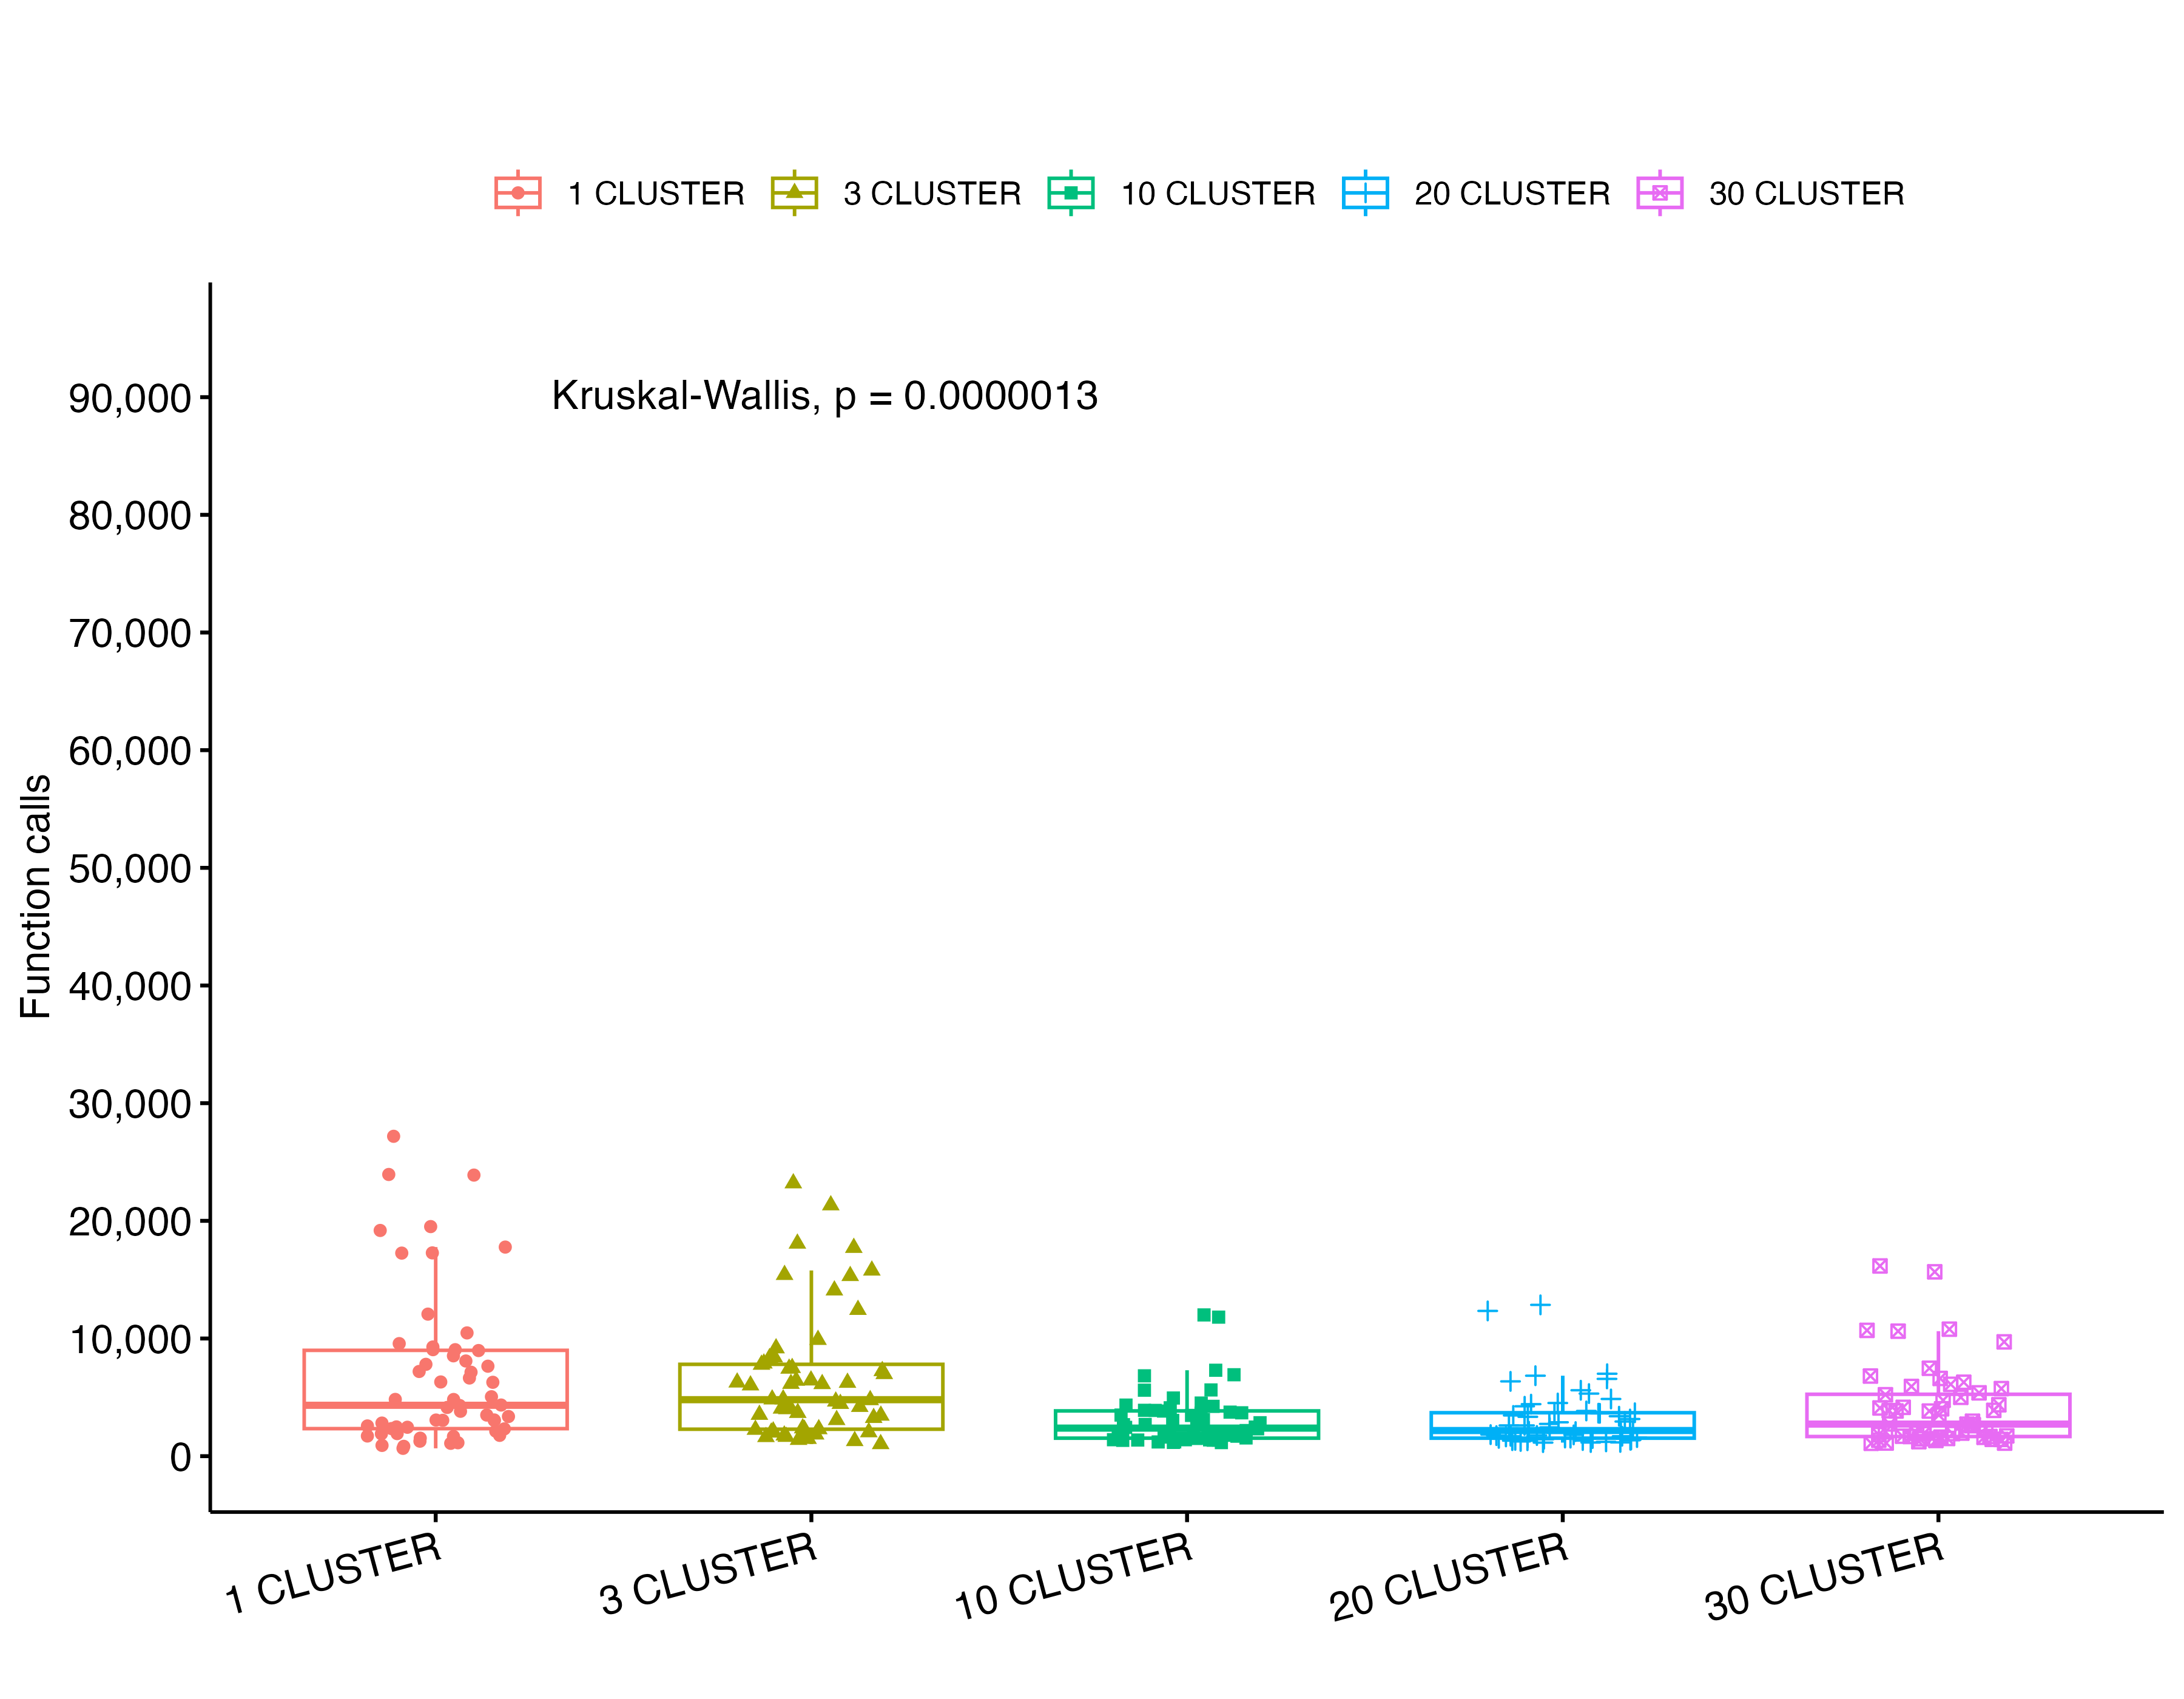
\includegraphics[scale=0.6]{subpopulation}

\caption{Impact of the Number of Clusters.\label{fig:Impact-of-the}}

\end{figure}

The diagram of Figure \ref{fig:Impact-of-the} shows the effect of
the number of clusters on the performance of the algorithm. Specifically,
the cases of 1, 3, 10, 20 and 30 clusters are compared. It is observed
that the use of more subpopulations reduces the number of function
calls, with the cases of 10 and 20 clusters showing the smallest values.
On the contrary, when only 1 cluster is used the method shows greater
dispersion and higher values, which indicates lower efficiency. The
Kruskal--Wallis statistical test (p = 0.0000013) shows that there
are statistically significant differences between different numbers
of clusters. Therefore, the results show that using an appropriate
number of subpopulations can improve the performance and convergence
speed of the algorithm.

\subsection{Impact of Propagation Mechanism}

Table \ref{tab:4.4 Impact of Propagation Mechanism} presents the
comparative evaluation of the proposed method with and without the
propagation mechanism (PROP = 0 and PROP = 1) in terms of average
objective function evaluations over benchmark functions of dimensions
25, 50, 100 and 150. The PROP parameter indicates the presence or
absence of the information propagation mechanism between the subpopulations:
the case PROP = 0 corresponds to execution without propagation, while
the case PROP = 1 corresponds to execution with propagation enabled.
The results show that the activation of the propagation mechanism
leads, in almost all the examined functions and dimensions to a reduction
in the number of evaluations compared to the corresponding execution
without propagation. For example, in the Büche Rastrigin\_150 function
the number of evaluations is reduced from 22453 to 6828, in the Sharp
Ridge\_150 from 10708 to 3034 while in the Zakharov\_150 from 9869
to 1539. The improvement is correspondingly significant in lower dimensions,
which suggests that the propagation mechanism not only favors large-scale
problems but also improves the overall behavior of the method. The
total number of function calls is reduced from about 493,939 in the
case without propagation (PROP = 0) to about 173,392 in the case with
propagation (PROP = 1). This difference corresponds to a significant
reduction in the overall computational cost and confirms that information
propagation between subpopulations is an important mechanism for improving
the efficiency of the proposed method. Overall, the results show that
the integration of the propagation mechanism enhances the computational
behavior of the algorithm, reducing the number of required objective
function evaluations and improving efficiency.

{\scriptsize{}
\begin{table}[H]
{\scriptsize\caption{Comparison of the proposed method with and without propagation mechanism
in terms of average objective function evaluations.\label{tab:4.4 Impact of Propagation Mechanism}}
}{\scriptsize\par}
\centering{}{\small{}%
\begin{tabular}{|c|c|c|}
\hline 
{\small\textbf{FUNCTION}} & {\small\textbf{PROP=0}} & {\small\textbf{PROP=1}}\tabularnewline
\hline 
\hline 
\begin{cellvarwidth}[t]
\centering
{\small ATTRACTIVE}{\small\par}

{\small SECTOR\_25}
\end{cellvarwidth} & {\small 1745} & {\small 1171}\tabularnewline
\hline 
\begin{cellvarwidth}[t]
\centering
{\small ATTRACTIVE}{\small\par}

{\small SECTOR\_50}
\end{cellvarwidth} & {\small 2162} & {\small 1549}\tabularnewline
\hline 
\begin{cellvarwidth}[t]
\centering
{\small ATTRACTIVE}{\small\par}

{\small SECTOR\_100}
\end{cellvarwidth} & {\small 2414} & {\small 1818}\tabularnewline
\hline 
\begin{cellvarwidth}[t]
\centering
{\small ATTRACTIVE}{\small\par}

{\small SECTOR\_150}
\end{cellvarwidth} & {\small 2440} & {\small 1754}\tabularnewline
\hline 
{\small BUCHE RASTRIGIN\_25} & {\small 8599} & {\small 1606}\tabularnewline
\hline 
{\small BUCHE RASTRIGIN\_50} & {\small 14282} & {\small 4514}\tabularnewline
\hline 
{\small BUCHE RASTRIGIN\_100} & {\small 20788} & {\small 7302}\tabularnewline
\hline 
{\small BUCHE RASTRIGIN\_150} & {\small 22453(0.97)} & {\small 6828}\tabularnewline
\hline 
{\small DISCUS\_25} & {\small 1809} & {\small 1221}\tabularnewline
\hline 
{\small DISCUS\_50} & {\small 2022} & {\small 1513}\tabularnewline
\hline 
{\small DISCUS\_100} & {\small 2392} & {\small 1827}\tabularnewline
\hline 
{\small DISCUS\_150} & {\small 2349} & {\small 1776}\tabularnewline
\hline 
{\small DIFFERENTPOWERS\_25} & {\small 9905} & {\small 1623}\tabularnewline
\hline 
{\small DIFFERENTPOWERS\_50} & {\small 16094} & {\small 6920}\tabularnewline
\hline 
{\small DIFFERENTPOWERS\_100} & {\small 26466} & {\small 11816}\tabularnewline
\hline 
{\small DIFFERENTPOWERS\_150} & {\small 33123} & {\small 12003}\tabularnewline
\hline 
{\small ELLIPSOIDAL\_25} & {\small 5003} & {\small 1216}\tabularnewline
\hline 
{\small ELLIPSOIDAL\_50} & {\small 9973} & {\small 2176}\tabularnewline
\hline 
{\small ELLIPSOIDAL\_100} & {\small 20082} & {\small 3833}\tabularnewline
\hline 
{\small ELLIPSOIDAL\_150} & {\small 27981} & {\small 4341}\tabularnewline
\hline 
{\small GALLAGHER21\_25} & {\small 2765} & {\small 1397}\tabularnewline
\hline 
{\small GALLAGHER21\_50} & {\small 3679(0.97)} & {\small 3095}\tabularnewline
\hline 
{\small GALLAGHER21\_100} & {\small 2044(0.53)} & {\small 3493(0.83)}\tabularnewline
\hline 
{\small GALLAGHER21\_150} & {\small 667(0.40)} & {\small 2472(0.73)}\tabularnewline
\hline 
{\small GALLAGHER101\_25} & {\small 2288(0.93)} & {\small 1209(0.93)}\tabularnewline
\hline 
{\small GALLAGHER101\_50} & {\small 3504(0.83)} & {\small 2447(0.73)}\tabularnewline
\hline 
{\small GALLAGHER101\_100} & {\small 4991(0.90)} & {\small 4235(0.93)}\tabularnewline
\hline 
{\small GALLAGHER101\_150} & {\small 5032} & {\small 3742(0.97)}\tabularnewline
\hline 
{\small GRIEWANK \_25} & {\small 5876} & {\small 1399}\tabularnewline
\hline 
{\small GRIEWANK \_50} & {\small 6446} & {\small 2675}\tabularnewline
\hline 
{\small GRIEWANK \_100} & {\small 7921} & {\small 4111}\tabularnewline
\hline 
{\small GRIEWANK \_150} & {\small 8657} & {\small 3897}\tabularnewline
\hline 
{\small GRIEWANK\_ROSENBROCK\_25} & {\small 6456} & {\small 1387}\tabularnewline
\hline 
{\small GRIEWANK\_ROSENBROCK\_50} & {\small 8186} & {\small 2696}\tabularnewline
\hline 
{\small GRIEWANK\_ROSENBROCK\_100} & {\small 9765} & {\small 3686}\tabularnewline
\hline 
{\small GRIEWANK\_ROSENBROCK\_150} & {\small 10496} & {\small 3463}\tabularnewline
\hline 
{\small ROSENBROCK\_25} & {\small 8468} & {\small 1364}\tabularnewline
\hline 
{\small ROSENBROCK\_50} & {\small 12829} & {\small 2842}\tabularnewline
\hline 
{\small ROSENBROCK\_100} & {\small 20141} & {\small 2842}\tabularnewline
\hline 
{\small ROSENBROCK\_150} & {\small 25818} & {\small 5628}\tabularnewline
\hline 
{\small RARSTIGIN\_25} & {\small 6901} & {\small 1535}\tabularnewline
\hline 
{\small RARSTIGIN\_50} & {\small 8901} & {\small 3888}\tabularnewline
\hline 
{\small RARSTIGIN\_100} & {\small 10440} & {\small 5608}\tabularnewline
\hline 
{\small RARSTIGIN\_150} & {\small 10149} & {\small 4942}\tabularnewline
\hline 
{\small STEP ELLIPSOIDAL\_25} & {\small 1351} & {\small 1154}\tabularnewline
\hline 
{\small STEP ELLIPSOIDAL\_50} & {\small 1623} & {\small 1507}\tabularnewline
\hline 
{\small STEP ELLIPSOIDAL\_100} & {\small 1769} & {\small 1737}\tabularnewline
\hline 
{\small STEP ELLIPSOIDAL\_150} & {\small 1720} & {\small 1698}\tabularnewline
\hline 
{\small SHARP RIDGE\_25} & {\small 7434} & {\small 1372}\tabularnewline
\hline 
{\small SHARP RIDGE\_50} & {\small 9092} & {\small 2322}\tabularnewline
\hline 
{\small SHARP RIDGE\_100} & {\small 10380} & {\small 3651}\tabularnewline
\hline 
{\small SHARP RIDGE\_150} & {\small 10708} & {\small 3034}\tabularnewline
\hline 
{\small ZAKHAROV\_25} & {\small 2631} & {\small 1355}\tabularnewline
\hline 
{\small ZAKHAROV\_50} & {\small 4674} & {\small 1819}\tabularnewline
\hline 
{\small ZAKHAROV\_100} & {\small 8186} & {\small 1344}\tabularnewline
\hline 
{\small ZAKHAROV\_150} & {\small 9869} & {\small 1539}\tabularnewline
\hline 
 & {\small 493939(0.97)} & {\small 173392(0.99)}\tabularnewline
\hline 
\end{tabular}}{\small\par}
\end{table}
}{\scriptsize\par}

\begin{figure}
\includegraphics[scale=0.6]{prop_0_1\lyxdot }

\caption{Impact of Propagation Mechanism. \label{fig:Impact-of-Propagation}}
\end{figure}

Figure \ref{fig:Impact-of-Propagation} shows the comparison of the
method when the propagation function is enabled and disabled. Specifically,
PROP = 1 indicates that propagation is enabled while PROP = 0 indicates
that the method is executed without propagation. It is observed that
when propagation is enabled (PROP = 1) the method requires significantly
fewer function calls and exhibits lower dispersion, which indicates
faster convergence. The comparison is performed using the paired Wilcoxon
statistical test, following the conventional star notation (ns: p
\textgreater{} 0.05, {*}: p \textless{} 0.05, {*}{*}: p \textless{}
0.01, {*}{*}{*}: p \textless{} 0.001, {*}{*}{*}{*}: p \textless{}
0.0001), where the overall result (p \textless{} 0.0001) shows that
the difference between the two cases is significant. Therefore, the
results show that enabling propagation improves the efficiency of
the proposed method.

It should be noted, however that the propagation mechanism introduces
additional communication overhead which is not explicitly reflected
in the number of function evaluations. Nevertheless this overhead
remains relatively low, as it mainly involves the exchange of a limited
number of high-quality solutions, and is therefore outweighed by the
significant gains in convergence efficiency observed in the experiments.
This observation is consistent with the overall reduction in computational
cost reported across the benchmark problems.

\subsection{Communication Strategy with 10 Subpopulations}

Table \ref{tab:4.5 Communication Strategy with 10 Subpopulations}
reports the average number of objective function evaluations obtained
under four different propagation strategies (1to1, 1toN, Nto1 and
NtoN) when 10 subpopulations are employed.\textbf{ }Lower values indicate
better performance with the best-performing value in each row highlighted
in bold for clarity. The results show that the NtoN strategy exhibits
the best computational behavior overall and leads to the smallest
function calls values in the vast majority of the functions examined.
For example, in the Büche Rastrigin\_150 function the NtoN strategy
requires 6828 function calls compared to 18787 for the 1to1 strategy,
10340 for 1toN and 11452 for Nto1. Correspondingly in Zakharov\_150
the NtoN strategy requires only 1539 function calls while the 1to1,
1toN and Nto1 strategies require 9158, 4352 and 4690, respectively.
Therefore the fully bidirectional information dissemination between
subpopulations enhances cooperation and facilitates faster diffusion
of useful information in the population. The 1toN and Nto1 strategies
also show improved behavior compared to the basic 1to1 approach. The
total number of function calls is 432,256 for the 1to1 strategy, 254,443
for 1toN, 274,853 for Nto1 and only 173,392 for NtoN. These results
show that, for the case of 10 subpopulations, the NtoN strategy is
the most efficient choice as it achieves the lowest overall computational
requirement.

{\scriptsize{}
\begin{table}[H]
{\scriptsize\caption{Comparison of propagation strategies under 10 subpopulations in terms
of average objective function evaluations.\label{tab:4.5 Communication Strategy with 10 Subpopulations}}
}{\scriptsize\par}

{\small{}%
\begin{tabular}{|c|c|c|c|c|}
\hline 
{\small\textbf{FUNCTION}} & {\small\textbf{1to1}} & {\small\textbf{1toN}} & {\small\textbf{Nto1}} & {\small\textbf{NtoN}}\tabularnewline
\hline 
\hline 
\begin{cellvarwidth}[t]
\centering
{\small ATTRACTIVE}{\small\par}

{\small SECTOR\_25}
\end{cellvarwidth} & {\small 1602} & {\small 1348} & {\small 1349} & {\small\textbf{1171}}\tabularnewline
\hline 
\begin{cellvarwidth}[t]
\centering
{\small ATTRACTIVE}{\small\par}

{\small SECTOR\_50}
\end{cellvarwidth} & {\small 2027} & {\small 1648} & {\small 1698} & {\small\textbf{1549}}\tabularnewline
\hline 
\begin{cellvarwidth}[t]
\centering
{\small ATTRACTIVE}{\small\par}

{\small SECTOR\_100}
\end{cellvarwidth} & {\small 2271} & {\small 1912} & {\small 1944} & {\small\textbf{1818}}\tabularnewline
\hline 
\begin{cellvarwidth}[t]
\centering
{\small ATTRACTIVE}{\small\par}

{\small SECTOR\_150}
\end{cellvarwidth} & {\small 2282} & {\small 1859} & {\small 1914} & {\small\textbf{1754}}\tabularnewline
\hline 
{\small BUCHE RASTRIGIN\_25} & {\small 7204} & {\small 3327} & {\small 3521} & {\small\textbf{1606}}\tabularnewline
\hline 
{\small BUCHE RASTRIGIN\_50} & {\small 11493(0.93)} & {\small 6203} & {\small 6789(0.97)} & {\small\textbf{4514}}\tabularnewline
\hline 
{\small BUCHE RASTRIGIN\_100} & {\small 17882} & {\small 10472} & {\small 11567} & {\small\textbf{7302}}\tabularnewline
\hline 
{\small BUCHE RASTRIGIN\_150} & {\small 18787(0.93)} & {\small 10340} & {\small 11452(0.97)} & {\small\textbf{6828}}\tabularnewline
\hline 
{\small DISCUS\_25} & {\small 1726} & {\small 1359} & {\small 1392} & {\small\textbf{1221}}\tabularnewline
\hline 
{\small DISCUS\_50} & {\small 1923} & {\small 1517} & {\small 1706} & {\small\textbf{1513}}\tabularnewline
\hline 
{\small DISCUS\_100} & {\small 2059} & {\small 1911} & {\small\textbf{1691}} & {\small 1827}\tabularnewline
\hline 
{\small DISCUS\_150} & {\small 2088} & {\small 1822} & {\small\textbf{1743}} & {\small 1776}\tabularnewline
\hline 
{\small DIFFERENTPOWERS\_25} & {\small 8481} & {\small 3981} & {\small 4630} & {\small\textbf{1623}}\tabularnewline
\hline 
{\small DIFFERENTPOWERS\_50} & {\small 14513} & {\small 9641} & {\small 9649} & {\small\textbf{6920}}\tabularnewline
\hline 
{\small DIFFERENTPOWERS\_100} & {\small 23558} & {\small 15731} & {\small 17144} & {\small\textbf{11816}}\tabularnewline
\hline 
{\small DIFFERENTPOWERS\_150} & {\small 28561} & {\small 16633} & {\small 18553} & {\small\textbf{12003}}\tabularnewline
\hline 
{\small ELLIPSOIDAL\_25} & {\small 4112} & {\small 2151} & {\small 2353} & {\small\textbf{1216}}\tabularnewline
\hline 
{\small ELLIPSOIDAL\_50} & {\small 8553} & {\small 3614} & {\small 4283} & {\small\textbf{2176}}\tabularnewline
\hline 
{\small ELLIPSOIDAL\_100} & {\small 16965} & {\small 6082} & {\small 7615} & {\small\textbf{3833}}\tabularnewline
\hline 
{\small ELLIPSOIDAL\_150} & {\small 22798} & {\small 7751} & {\small 9556} & {\small\textbf{4341}}\tabularnewline
\hline 
{\small GALLAGHER21\_25} & {\small 2319} & {\small 1692} & {\small 1689} & {\small\textbf{1397}}\tabularnewline
\hline 
{\small GALLAGHER21\_50} & {\small 3201(0.93)} & {\small 3137(0.97)} & {\small\textbf{2914(0.93)}} & {\small 3095}\tabularnewline
\hline 
{\small GALLAGHER21\_100} & {\small 2419(0.60)} & {\small 3273(0.77)} & {\small\textbf{2476(0.63)}} & {\small 3493(0.83)}\tabularnewline
\hline 
{\small GALLAGHER21\_150} & {\small\textbf{1079(0.47)}} & {\small 1507(0.53)} & {\small 1245(0.50)} & {\small 2472(0.73)}\tabularnewline
\hline 
{\small GALLAGHER101\_25} & {\small 2148} & {\small 1580(0.97)} & {\small 1636} & {\small\textbf{1209(0.93)}}\tabularnewline
\hline 
{\small GALLAGHER101\_50} & {\small 3777(0.97)} & {\small 3572(0.97)} & {\small 3335(0.93)} & {\small\textbf{2447(0.73)}}\tabularnewline
\hline 
{\small GALLAGHER101\_100} & {\small 5272} & {\small 4891} & {\small 4729(0.97)} & {\small\textbf{4235(0.93)}}\tabularnewline
\hline 
{\small GALLAGHER101\_150} & {\small 4785} & {\small 4282} & {\small 4429} & {\small\textbf{3742(0.97)}}\tabularnewline
\hline 
{\small GRIEWANK \_25} & {\small 5277} & {\small 2780} & {\small 3232} & {\small\textbf{1399}}\tabularnewline
\hline 
{\small GRIEWANK \_50} & {\small 5682} & {\small 3384} & {\small 3679} & {\small\textbf{2675}}\tabularnewline
\hline 
{\small GRIEWANK \_100} & {\small 6813} & {\small 4314} & {\small 4799} & {\small\textbf{4111}}\tabularnewline
\hline 
{\small GRIEWANK \_150} & {\small 7549} & {\small 4274} & {\small 4541(0.87)} & {\small\textbf{3897}}\tabularnewline
\hline 
{\small GRIEWANK\_ROSENBROCK\_25} & {\small 5722} & {\small 2966} & {\small 3467(0.97)} & {\small\textbf{1387}}\tabularnewline
\hline 
{\small GRIEWANK\_ROSENBROCK\_50} & {\small 7311} & {\small 4285} & {\small 4700(0.97)} & {\small\textbf{2696}}\tabularnewline
\hline 
{\small GRIEWANK\_ROSENBROCK\_100} & {\small 8723} & {\small 5430} & {\small 6023} & {\small\textbf{3686}}\tabularnewline
\hline 
{\small GRIEWANK\_ROSENBROCK\_150} & {\small 9517} & {\small 5367} & {\small 5802} & {\small\textbf{3463}}\tabularnewline
\hline 
{\small ROSENBROCK\_25} & {\small 7668} & {\small 3471} & {\small 4288} & {\small\textbf{1364}}\tabularnewline
\hline 
{\small ROSENBROCK\_50} & {\small 11170} & {\small 5907} & {\small 6752} & {\small\textbf{2842}}\tabularnewline
\hline 
{\small ROSENBROCK\_100} & {\small 17250} & {\small 10773} & {\small 11768} & {\small\textbf{2842}}\tabularnewline
\hline 
{\small ROSENBROCK\_150} & {\small 23256} & {\small 12622} & {\small 14393} & {\small\textbf{5628}}\tabularnewline
\hline 
{\small RARSTIGIN\_25} & {\small 5500} & {\small 2935} & {\small 3295} & {\small\textbf{1535}}\tabularnewline
\hline 
{\small RARSTIGIN\_50} & {\small 7523} & {\small 5364} & {\small 4541} & {\small\textbf{3888}}\tabularnewline
\hline 
{\small RARSTIGIN\_100} & {\small 8597(0.97)} & {\small 6728} & {\small 6790} & {\small\textbf{5608}}\tabularnewline
\hline 
{\small RARSTIGIN\_150} & {\small 8784(0.97)} & {\small 6025(0.97)} & {\small 6138} & {\small\textbf{4942}}\tabularnewline
\hline 
{\small STEP ELLIPSOIDAL\_25} & {\small 1328} & {\small 1205} & {\small 1207} & {\small\textbf{1154}}\tabularnewline
\hline 
{\small STEP ELLIPSOIDAL\_50} & {\small 1593} & {\small 1530} & {\small 1524} & {\small\textbf{1507}}\tabularnewline
\hline 
{\small STEP ELLIPSOIDAL\_100} & {\small 1742} & {\small\textbf{1735}} & {\small 1743} & {\small 1737}\tabularnewline
\hline 
{\small STEP ELLIPSOIDAL\_150} & {\small 1713} & {\small 1701} & {\small 1723} & {\small\textbf{1698}}\tabularnewline
\hline 
{\small SHARP RIDGE\_25} & {\small 6833} & {\small 3248} & {\small 3390} & {\small\textbf{1372}}\tabularnewline
\hline 
{\small SHARP RIDGE\_50} & {\small 7629} & {\small 3917} & {\small 4348} & {\small\textbf{2322}}\tabularnewline
\hline 
{\small SHARP RIDGE\_100} & {\small 8889} & {\small 4814} & {\small 5363} & {\small\textbf{3651}}\tabularnewline
\hline 
{\small SHARP RIDGE\_150} & {\small 9656} & {\small 4522} & {\small 5010} & {\small\textbf{3034}}\tabularnewline
\hline 
{\small ZAKHAROV\_25} & {\small 2407} & {\small 1682} & {\small 1850} & {\small\textbf{1355}}\tabularnewline
\hline 
{\small ZAKHAROV\_50} & {\small 4004} & {\small 2579} & {\small 2651} & {\small\textbf{1819}}\tabularnewline
\hline 
{\small ZAKHAROV\_100} & {\small 7077} & {\small 3297} & {\small 4144} & {\small\textbf{1344}}\tabularnewline
\hline 
{\small ZAKHAROV\_150} & {\small 9158} & {\small 4352} & {\small 4690} & {\small\textbf{1539}}\tabularnewline
\hline 
 & {\small 432256(0.98)} & {\small 254443(0.99)} & {\small 274853(0.98)} & {\small 173392(0.99)}\tabularnewline
\hline 
\end{tabular}}{\small\par}
\end{table}
}{\scriptsize\par}

\begin{figure}
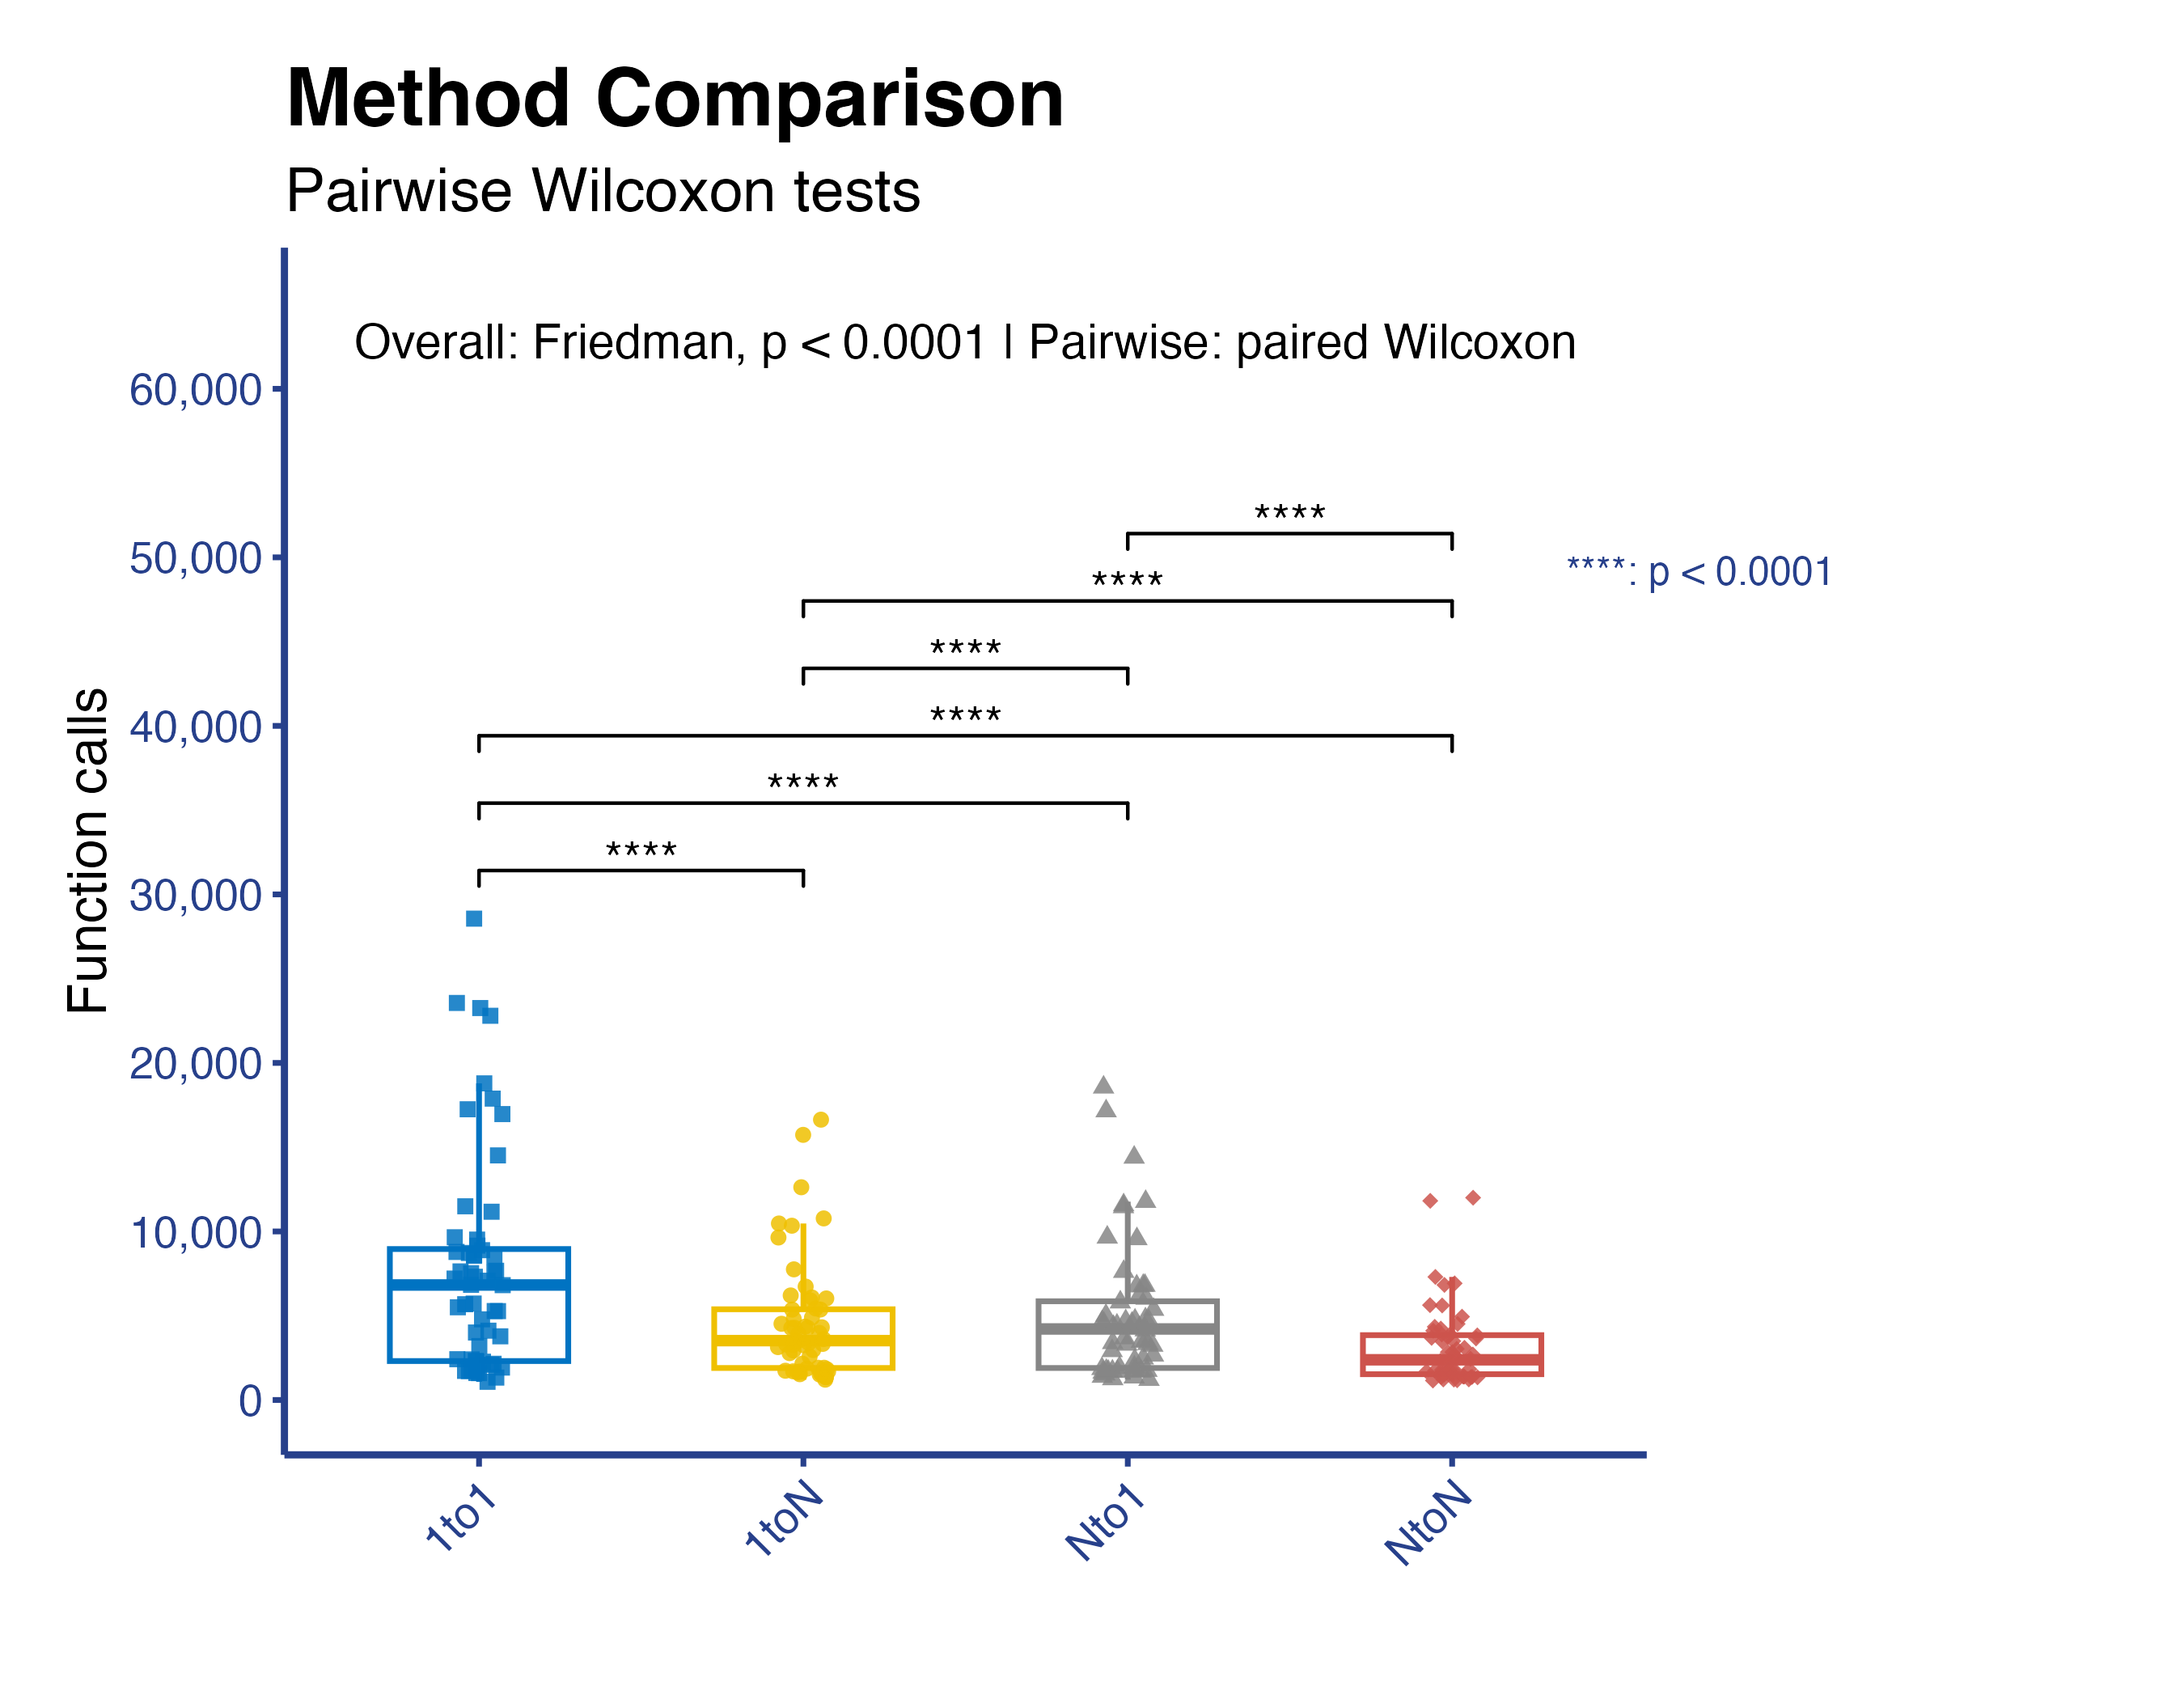
\includegraphics[scale=0.6]{sub10}

\caption{Communication Strategy with 10 Subpopulations.\label{fig:Communication-Strategy-with}}

\end{figure}

Figure \ref{fig:Communication-Strategy-with} shows the comparison
of different communication modes between subpopulations when 10 clusters
are used, based on the number of function calls. The configurations
examined are 1to1, 1toN, Nto1 and NtoN which express different information
dissemination schemes between subpopulations. It is observed that
the NtoN configuration presents the lowest values and the smallest
dispersion, which indicates faster convergence of the algorithm. On
the contrary, the 1to1 case presents a higher number of function calls.
The overall statistical analysis was performed with the Friedman test
(p \textless{} 0.0001) while the individual comparisons were performed
with paired Wilcoxon tests following the conventional star notation
(ns: p \textgreater{} 0.05, {*}: p \textless{} 0.05, {*}{*}: p \textless{}
0.01, {*}{*}{*}: p \textless{} 0.001, {*}{*}{*}{*}: p \textless{}
0.0001). The presence of {*}{*}{*}{*} (p \textless{} 0.0001) indicates
that the differences between the methods are statistically significant.
The results suggest that the exchange of information between all subpopulations
is significant.

\subsection{Communication Strategy with 20 Subpopulations}

Table \ref{tab:4.6 Communication Strategy with 20 Subpopulations}
presents the corresponding results for the same propagation strategies
when 20 subpopulations are utilized. Lower values indicate better
performance, with the best-performing value in each row highlighted
in bold for clarity. The results show that, also in the case of 20
subpopulations, the NtoN strategy displays the overall most efficient
behavior, as it achieves the lowest or among the lowest function calls
values. Indicatively, in the Rosenbrock\_150 function the NtoN strategy
requires 6356 function calls, compared to 23645 for 1to1, 8431 for
1toN and 11263 for Nto1. Accordingly, in Rastrigin\_150 the required
evaluations are reduced to 4861 for NtoN compared to 8674, 5954 and
5671 for the 1to1, 1toN and Nto1 strategies, respectively. These results
suggest that the fully cooperative form of propagation significantly
accelerates the diffusion of useful information between subpopulations
and facilitates convergence towards better regions of the search space.
The 1toN and Nto1 strategies also show improved behavior compared
to the basic 1to1 approach, which confirms that even partial information
propagation is beneficial for the search process. The total number
of function calls is 414,978 for the 1to1 strategy 195,980 for 1toN
222,989 for Nto1 and only 174,401 for NtoN. These results show that,
for the case of 20 subpopulations the NtoN strategy is again the most
efficient choice as it achieves the lowest overall computational requirement.

{\scriptsize{}
\begin{table}[H]
{\scriptsize\caption{Comparison of propagation strategies under 20 subpopulations in terms
of average objective function evaluations.\label{tab:4.6 Communication Strategy with 20 Subpopulations}}
}{\scriptsize\par}

{\small{}%
\begin{tabular}{|c|c|c|c|c|}
\hline 
{\small\textbf{FUNCTION}} & {\small\textbf{1to1}} & {\small\textbf{1toN}} & {\small\textbf{Nto1}} & {\small\textbf{NtoN}}\tabularnewline
\hline 
\hline 
\begin{cellvarwidth}[t]
\centering
{\small ATTRACTIVE}{\small\par}

{\small SECTOR\_25}
\end{cellvarwidth} & {\small 1663} & {\small 1317} & {\small 1271} & {\small\textbf{1170}}\tabularnewline
\hline 
\begin{cellvarwidth}[t]
\centering
{\small ATTRACTIVE}{\small\par}

{\small SECTOR\_50}
\end{cellvarwidth} & {\small 2026} & {\small 1582} & {\small 1644} & {\small\textbf{1534}}\tabularnewline
\hline 
\begin{cellvarwidth}[t]
\centering
{\small ATTRACTIVE}{\small\par}

{\small SECTOR\_100}
\end{cellvarwidth} & {\small 2247} & {\small 1826} & {\small 1893} & {\small\textbf{1809}}\tabularnewline
\hline 
\begin{cellvarwidth}[t]
\centering
{\small ATTRACTIVE}{\small\par}

{\small SECTOR\_150}
\end{cellvarwidth} & {\small 2231} & {\small 1797} & {\small 1898} & {\small\textbf{1754}}\tabularnewline
\hline 
{\small BUCHE RASTRIGIN\_25} & {\small 7185} & {\small 2674} & {\small 2768} & {\small\textbf{1578}}\tabularnewline
\hline 
{\small BUCHE RASTRIGIN\_50} & {\small 11071(0.97)} & {\small 5436(0.97)} & {\small 5108(0.87)} & {\small\textbf{4420(0.97)}}\tabularnewline
\hline 
{\small BUCHE RASTRIGIN\_100} & {\small 15630(0.90)} & {\small 7698(0.97)} & {\small 8794(0.83)} & {\small\textbf{7006(0.97)}}\tabularnewline
\hline 
{\small BUCHE RASTRIGIN\_150} & {\small 17743(0.97)} & {\small 7296(0.90)} & {\small 8690(0.87)} & {\small\textbf{6837(0.97)}}\tabularnewline
\hline 
{\small DISCUS\_25} & {\small 1721} & {\small 1222} & {\small 1330} & {\small\textbf{1153}}\tabularnewline
\hline 
{\small DISCUS\_50} & {\small 1833} & {\small 1413} & {\small\textbf{1368}} & {\small 1549}\tabularnewline
\hline 
{\small DISCUS\_100} & {\small 1803} & {\small 1642} & {\small\textbf{1555}} & {\small 1636}\tabularnewline
\hline 
{\small DISCUS\_150} & {\small 1927} & {\small 1601} & {\small\textbf{1572}} & {\small 1694}\tabularnewline
\hline 
{\small DIFFERENTPOWERS\_25} & {\small 9370} & {\small 3382} & {\small 3277} & {\small\textbf{2123}}\tabularnewline
\hline 
{\small DIFFERENTPOWERS\_50} & {\small 14912} & {\small 7296} & {\small 7985} & {\small\textbf{6567}}\tabularnewline
\hline 
{\small DIFFERENTPOWERS\_100} & {\small 23185} & {\small 12713} & {\small 14072} & {\small\textbf{12344}}\tabularnewline
\hline 
{\small DIFFERENTPOWERS\_150} & {\small 27829} & {\small 13781} & {\small 15957} & {\small\textbf{12858}}\tabularnewline
\hline 
{\small ELLIPSOIDAL\_25} & {\small 4242} & {\small 1600} & {\small 1805} & {\small\textbf{1216}}\tabularnewline
\hline 
{\small ELLIPSOIDAL\_50} & {\small 7652} & {\small 2879} & {\small 3370} & {\small\textbf{2173}}\tabularnewline
\hline 
{\small ELLIPSOIDAL\_100} & {\small 14835} & {\small 4172} & {\small 5690} & {\small\textbf{3843}}\tabularnewline
\hline 
{\small ELLIPSOIDAL\_150} & {\small 20040} & {\small 5562} & {\small 6949} & {\small\textbf{4518}}\tabularnewline
\hline 
{\small GALLAGHER21\_25} & {\small 2347} & {\small 1542} & {\small 1582} & {\small\textbf{1376}}\tabularnewline
\hline 
{\small GALLAGHER21\_50} & {\small 2609(0.80)} & {\small 2656(0.93)} & {\small\textbf{2031(0.80)}} & {\small 2740(0.93)}\tabularnewline
\hline 
{\small GALLAGHER21\_100} & {\small\textbf{1250(0.40)}} & {\small 2255(0.60)} & {\small 1725(0.50)} & {\small 3157(0.80)}\tabularnewline
\hline 
{\small GALLAGHER21\_150} & {\small\textbf{654(0.40)}} & {\small 1343(0.50)} & {\small 1019(0.47)} & {\small 2087(0.63)}\tabularnewline
\hline 
{\small GALLAGHER101\_25} & {\small 2180} & {\small 1383(0.97)} & {\small 1630} & {\small\textbf{1252(0.93)}}\tabularnewline
\hline 
{\small GALLAGHER101\_50} & {\small 3554(0.90)} & {\small 2894(0.87)} & {\small 2899(0.90)} & {\small\textbf{2612(0.77)}}\tabularnewline
\hline 
{\small GALLAGHER101\_100} & {\small 4806(0.87)} & {\small 3942(0.83)} & {\small 3927(0.83)} & {\small\textbf{3651(0.87)}}\tabularnewline
\hline 
{\small GALLAGHER101\_150} & {\small 5034} & {\small 4093(0.97)} & {\small 3804(0.93)} & {\small\textbf{3688(0.97)}}\tabularnewline
\hline 
{\small GRIEWANK \_25} & {\small 5255} & {\small 2219} & {\small 2341} & {\small\textbf{1345}}\tabularnewline
\hline 
{\small GRIEWANK \_50} & {\small 5545} & {\small 3050} & {\small 3292} & {\small\textbf{2612}}\tabularnewline
\hline 
{\small GRIEWANK \_100} & {\small 6280} & {\small\textbf{3760}} & {\small 3823} & {\small 4239}\tabularnewline
\hline 
{\small GRIEWANK \_150} & {\small 6933} & {\small\textbf{3596}} & {\small 3887} & {\small 3704}\tabularnewline
\hline 
{\small GRIEWANK\_ROSENBROCK\_25} & {\small 5566} & {\small 1851} & {\small 2653} & {\small\textbf{1434}}\tabularnewline
\hline 
{\small GRIEWANK\_ROSENBROCK\_50} & {\small 7156} & {\small 3145} & {\small 3754} & {\small\textbf{2446}}\tabularnewline
\hline 
{\small GRIEWANK\_ROSENBROCK\_100} & {\small 8461} & {\small 3983} & {\small 4858} & {\small\textbf{3641}}\tabularnewline
\hline 
{\small GRIEWANK\_ROSENBROCK\_150} & {\small 8923} & {\small 3773} & {\small 4887} & {\small\textbf{3394}}\tabularnewline
\hline 
{\small ROSENBROCK\_25} & {\small 7197} & {\small 1876} & {\small 2995} & {\small\textbf{1311}}\tabularnewline
\hline 
{\small ROSENBROCK\_50} & {\small 10930} & {\small 3825} & {\small 5192} & {\small\textbf{2944}}\tabularnewline
\hline 
{\small ROSENBROCK\_100} & {\small 17190} & {\small 6262} & {\small 9295} & {\small\textbf{5602}}\tabularnewline
\hline 
{\small ROSENBROCK\_150} & {\small 23645} & {\small 8431} & {\small 11263} & {\small\textbf{6356}}\tabularnewline
\hline 
{\small RARSTIGIN\_25} & {\small 5727} & {\small 1985} & {\small 2346} & {\small\textbf{1542}}\tabularnewline
\hline 
{\small RARSTIGIN\_50} & {\small 6901(0.93)} & {\small 4141(0.97)} & {\small 4157(0.93)} & {\small\textbf{3461(0.93)}}\tabularnewline
\hline 
{\small RARSTIGIN\_100} & {\small 8313(0.93)} & {\small 5491(0.90)} & {\small 5433(0.87)} & {\small\textbf{5318}}\tabularnewline
\hline 
{\small RARSTIGIN\_150} & {\small 8674(0.97)} & {\small 5954(0.90)} & {\small 5671(0.97)} & {\small\textbf{4861(0.97)}}\tabularnewline
\hline 
{\small STEP ELLIPSOIDAL\_25} & {\small 1342} & {\small 1238} & {\small 1198} & {\small\textbf{1160}}\tabularnewline
\hline 
{\small STEP ELLIPSOIDAL\_50} & {\small 1557} & {\small 1516} & {\small 1539} & {\small\textbf{1500}}\tabularnewline
\hline 
{\small STEP ELLIPSOIDAL\_100} & {\small 1772} & {\small\textbf{1733}} & {\small\textbf{1733}} & {\small 1745}\tabularnewline
\hline 
{\small STEP ELLIPSOIDAL\_150} & {\small 1727} & {\small 1705} & {\small 1706} & {\small\textbf{1691}}\tabularnewline
\hline 
{\small SHARP RIDGE\_25} & {\small 6774} & {\small 2150} & {\small 2645} & {\small\textbf{1329}}\tabularnewline
\hline 
{\small SHARP RIDGE\_50} & {\small 7431} & {\small 2899} & {\small 3598} & {\small\textbf{2184}}\tabularnewline
\hline 
{\small SHARP RIDGE\_100} & {\small 8358} & {\small 4010} & {\small 4411} & {\small\textbf{3345}}\tabularnewline
\hline 
{\small SHARP RIDGE\_150} & {\small 8713} & {\small 3680} & {\small 4186} & {\small\textbf{2880}}\tabularnewline
\hline 
{\small ZAKHAROV\_25} & {\small 2338} & {\small 1391} & {\small 1557} & {\small\textbf{1351}}\tabularnewline
\hline 
{\small ZAKHAROV\_50} & {\small 4005} & {\small 1845} & {\small 2371} & {\small\textbf{1830}}\tabularnewline
\hline 
{\small ZAKHAROV\_100} & {\small 6815} & {\small 1687} & {\small 2836} & {\small\textbf{1318}}\tabularnewline
\hline 
{\small ZAKHAROV\_150} & {\small 9871} & {\small 1787} & {\small 3749} & {\small\textbf{1513}}\tabularnewline
\hline 
 & {\small 414978(0.97)} & {\small 195980(0.97)} & {\small 222989(0.96)} & {\small 174401(0.98)}\tabularnewline
\hline 
\end{tabular}}{\small\par}
\end{table}
}{\scriptsize\par}

\begin{figure}
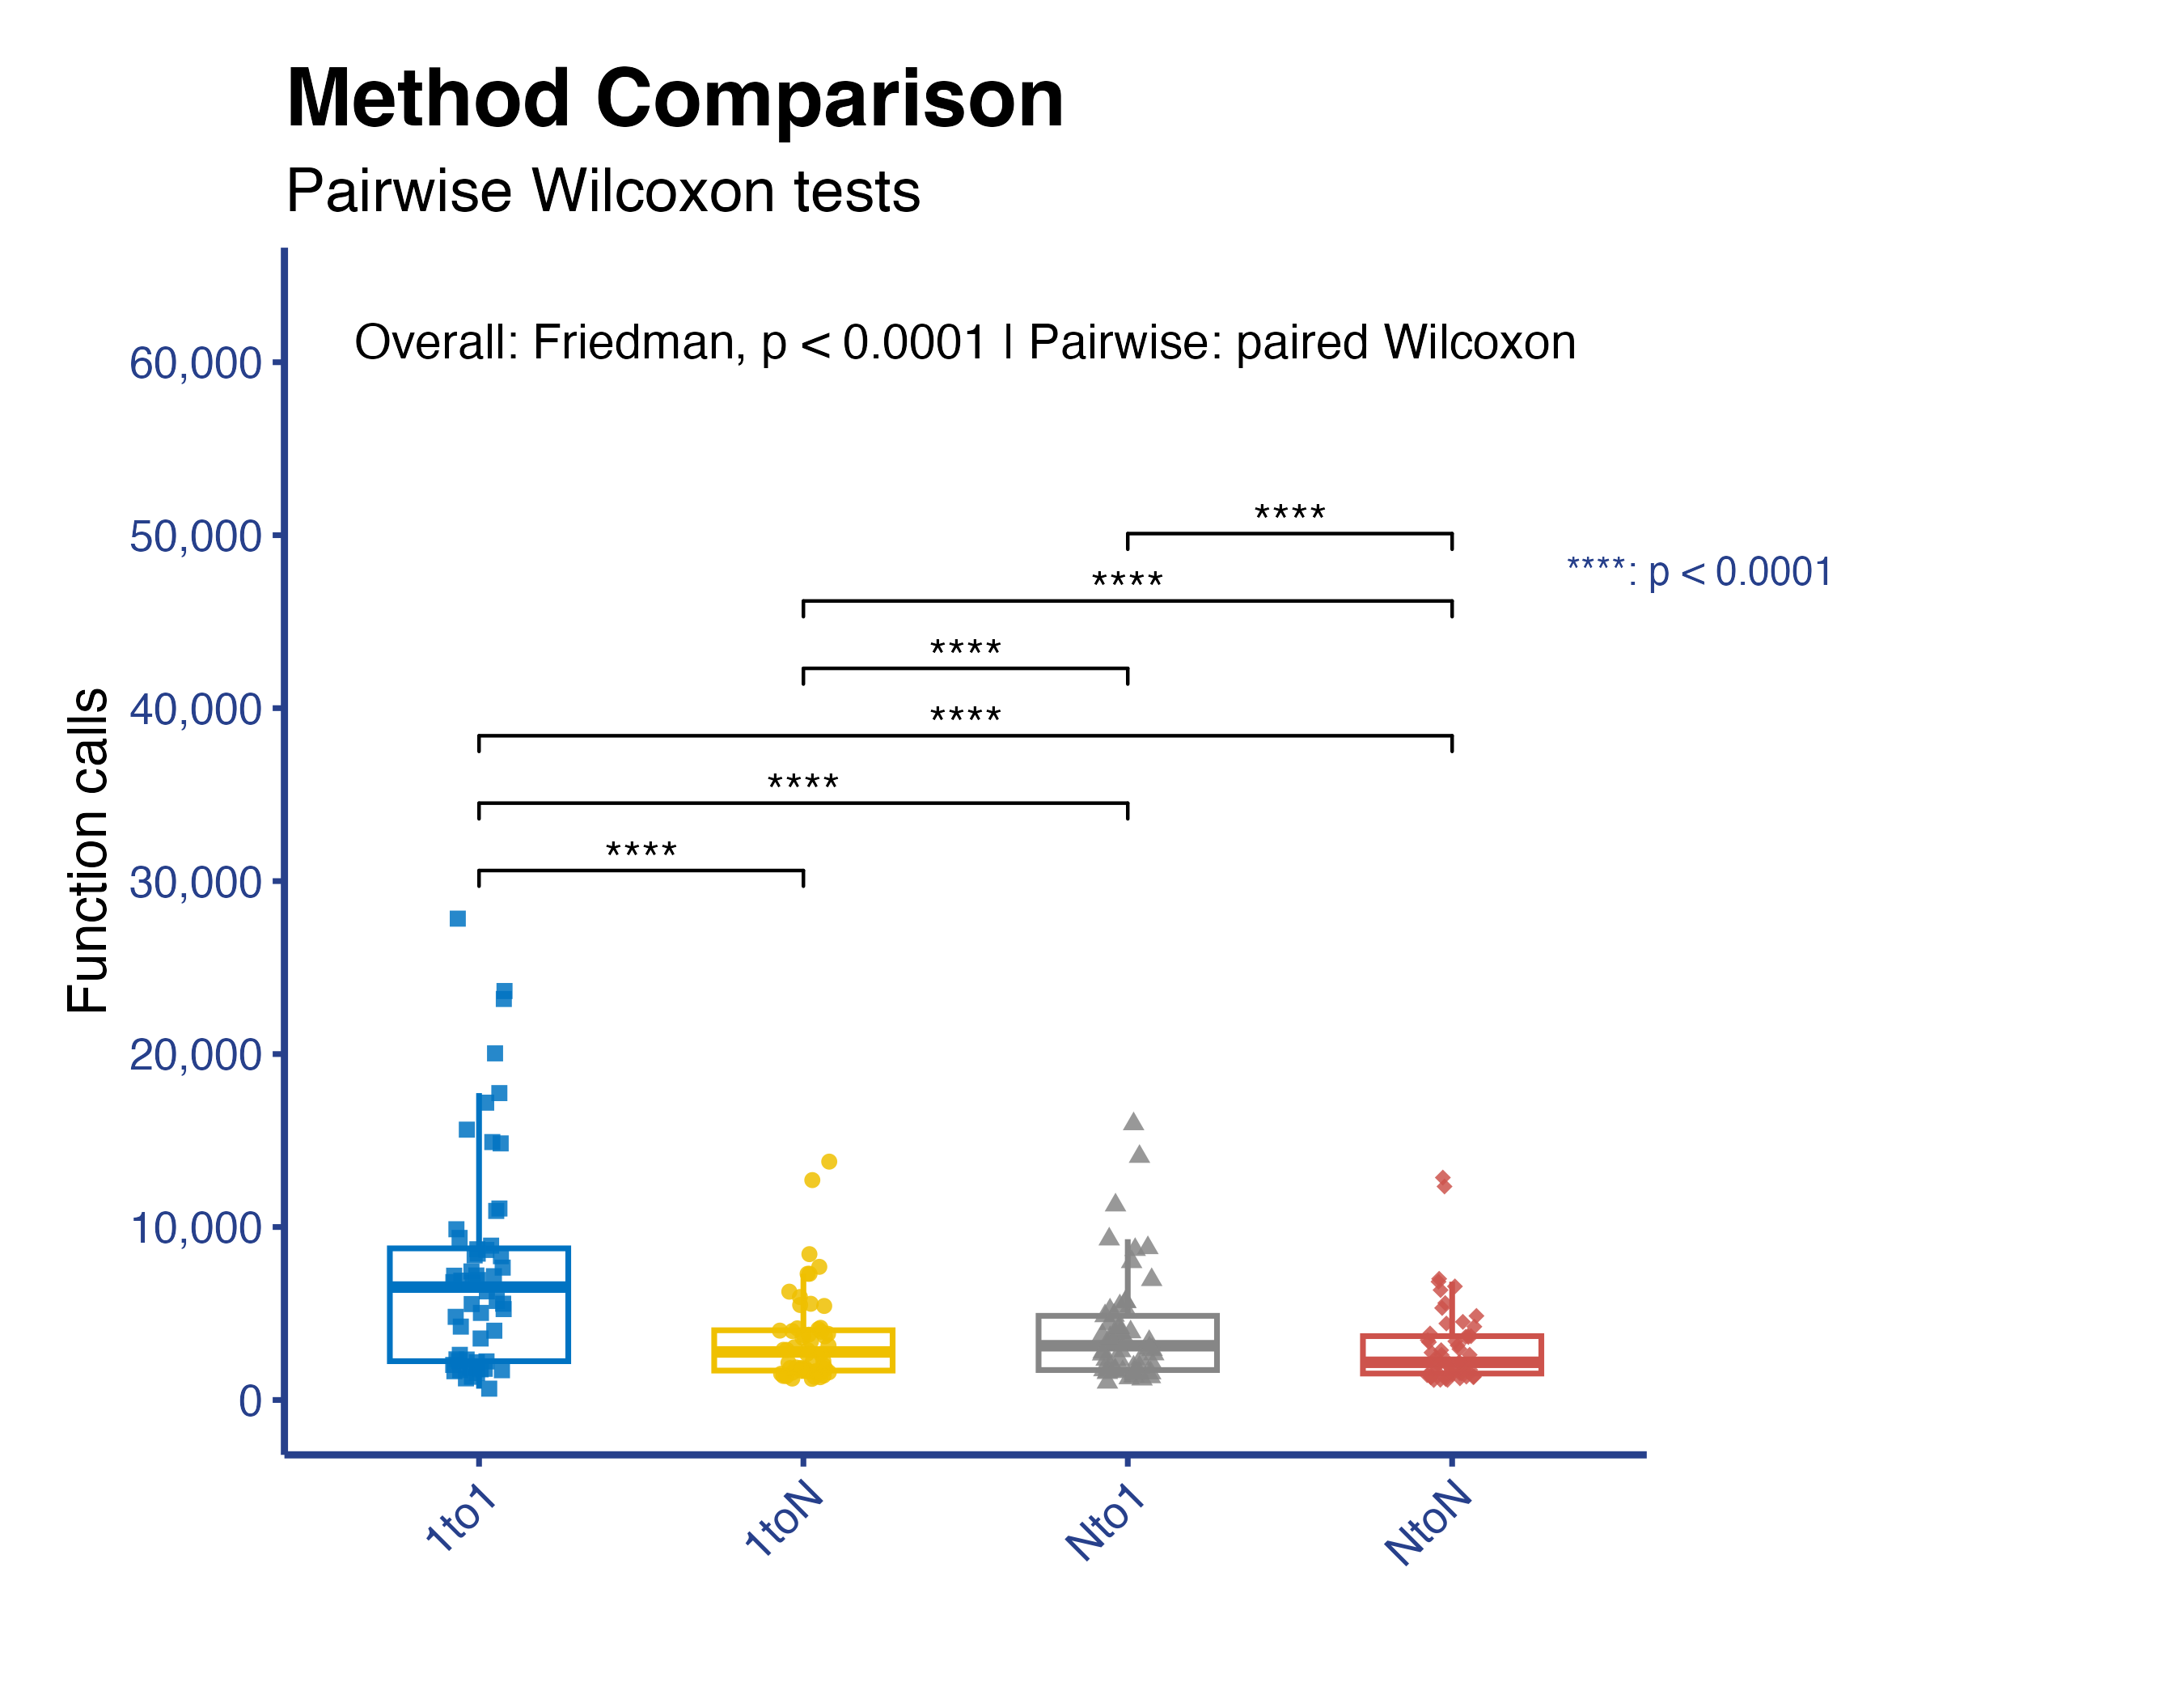
\includegraphics[scale=0.6]{sub20}

\caption{Communication Strategy with 20 Subpopulations.\label{fig:Communication-Strategy-with-1}}

\end{figure}

Figure \ref{fig:Communication-Strategy-with-1} shows the comparison
of different communication modes between subpopulations when 20 clusters
are used, based on the number of function calls. The configurations
examined are 1to1, 1toN, Nto1 and NtoN which express different information
dissemination schemes between subpopulations. It is observed that
the NtoN configuration presents the lowest values \LyXZeroWidthSpace\LyXZeroWidthSpace and
the smallest dispersion, which indicates faster convergence of the
algorithm. On the contrary, the 1to1 case presents a higher number
of function calls. The overall statistical analysis was performed
with the Friedman test (p \textless{} 0.0001) while the individual
comparisons were performed with paired Wilcoxon tests, following the
conventional star notation (ns: p \textgreater{} 0.05, {*}: p \textless{}
0.05, {*}{*}: p \textless{} 0.01, {*}{*}{*}: p \textless{} 0.001,
{*}{*}{*}{*}: p \textless{} 0.0001). The presence of {*}{*}{*}{*}
(p \textless{} 0.0001) indicates that the differences between the
methods are statistically significant. The results suggest that the
exchange of information between all subpopulations is significant.

A combined analysis of the communication strategies for both 10 and
20 subpopulations shows that the NtoN scheme consistently achieves
the best performance in terms of objective function evaluations. However,
it should be noted that this conclusion is based primarily on evaluation
efficiency, as runtime and communication overhead have not been explicitly
measured. The improved performance of the NtoN strategy can be explained
by its fully cooperative communication mechanism, which enables rapid
dissemination of high-quality solutions across all subpopulations.
This leads to more stable convergence behavior and increased robustness,
as promising regions of the search space are more effectively exploited.
In contrast, more limited communication schemes restrict information
flow, resulting in slower convergence and higher variability. Although
the NtoN strategy introduces additional communication operations,
this overhead is relatively small compared to the cost of objective
function evaluations, especially in high-dimensional problems. Therefore,
NtoN can be considered the most effective strategy in terms of solution
quality and robustness, while its optimality should be interpreted
within the context of evaluation-based performance rather than strict
computational cost.

\subsection{The proposed method in comparison with other methods}

To provide a more rigorous and statistically sound evaluation of the
proposed method, the results are reported in terms of the mean and
standard deviation (mean \textpm{} std) of the final objective function
values over 30 independent runs. This allows for a comprehensive assessment
of both solution quality and robustness. The proposed method consistently
achieves competitive or superior final objective values accompanied
by low variance across independent runs. This indicates not only high
accuracy but also stable and reliable convergence behavior compared
to the examined algorithms.

Table \ref{tab:The proposed method in comparison with others} presents
the comparative performance of the proposed method against established
metaheuristic algorithms, namely GA, DE, GWO, ParallelDE, SAOP, BGWO
and WOA, in terms of average objective function evaluations over benchmark
functions of dimensions 25, 50, 100 and 150. Lower values indicate
superior optimization efficiency. The results show that the proposed
method shows the best performance most of the time. Indicatively in
the Zakharov\_150 function the proposed method requires 1539 evaluations,
compared to 38858 for GA, 14744 for DE, 3251 for GWO, 5613 for ParallelDE,
4341 for SAOP, 3333 for BGWO and 11943 for WOA. Correspondingly, on
Sharp Ridge\_150 the proposed method achieves 3034 function calls,
compared to 12266, 12231, 25399, 5614, 4055, 24923 and 8022 respectively.
Particularly important is the fact that the proposed approach maintains
its efficiency not only in complex and multimodal problems, but also
in functions of different structure presenting consistently low computational
cost across the entire range of dimensions. The total number of function
calls of the proposed method amounts to 173,392, compared to 777,899
for GA, 762,504 for DE, 772,866 for GWO, 314,144 for ParallelDE, 263,370
for SAOP, 724,617 for BGWO and 371,962 for WOA. In conclusion, it
follows that the combination of the cooperative subpopulation structure
the information dissemination mechanism and the overall parallelized
search strategy substantially enhances the efficiency of the algorithm
making it particularly suitable for optimization and high-dimensional
problems.

{\scriptsize{}
\begin{table}[H]
\caption{Comparison of the proposed method against competing metaheuristic
algorithms in terms of average objective function evaluations.\label{tab:The proposed method in comparison with others}}

{\tiny{}%
\begin{tabular}{|c|c|c|c|c|c|c|c|c|}
\hline 
{\tiny\textbf{FUNCTION}} & {\tiny\textbf{GA}} & {\tiny\textbf{DE}} & {\tiny\textbf{GWO}} & {\tiny\textbf{PARALLELDE}} & {\tiny\textbf{SAOP}} & {\tiny\textbf{BGWO}} & {\tiny\textbf{WOA}} & {\tiny\textbf{PROPOSED}}\tabularnewline
\hline 
\hline 
\begin{cellvarwidth}[t]
\centering
{\tiny ATTRACTIVE}{\tiny\par}

{\tiny SECTOR\_25}
\end{cellvarwidth} & 2281 & 2234 & 3772 & 5594 & 1715 & 3239 & 1944 & 1171\tabularnewline
\hline 
\begin{cellvarwidth}[t]
\centering
{\tiny ATTRACTIVE}{\tiny\par}

{\tiny SECTOR\_50}
\end{cellvarwidth} & 2297 & 2298 & 12556 & 5611 & 2106 & 17575 & 4646 & 1549\tabularnewline
\hline 
\begin{cellvarwidth}[t]
\centering
{\tiny ATTRACTIVE}{\tiny\par}

{\tiny SECTOR\_100}
\end{cellvarwidth} & 2344 & 2273 & 29011 & 5623 & 2691 & 28735 & 6739 & 1818\tabularnewline
\hline 
\begin{cellvarwidth}[t]
\centering
{\tiny ATTRACTIVE}{\tiny\par}

{\tiny SECTOR\_150}
\end{cellvarwidth} & 2345 & 2255 & 25348 & 5614 & 2618 & 24872 & 6070 & 1754\tabularnewline
\hline 
{\tiny BUCHE RASTRIGIN\_25} & 11233(0.93) & 11417(0.93) & 4214 & 5592 & 2183(0.93) & 1989(0.93) & 3009(0.97) & 1606\tabularnewline
\hline 
{\tiny BUCHE RASTRIGIN\_50} & 17589(0.57) & 21873(0.57) & 13509(0.90) & 5610 & 4657(0.57) & 4033(0.57) & 14163(0.70) & 4514\tabularnewline
\hline 
{\tiny BUCHE RASTRIGIN\_100} & 32881(0.30) & 39401(0.30) & 23867(0.80) & 5622 & 7806(0.30) & 7564(0.30) & 7293(0.97) & 7302\tabularnewline
\hline 
{\tiny BUCHE RASTRIGIN\_150} & 36444(0.40) & 48017(0.40) & 22139(0.87) & 5611 & 7731(0.40) & 6472(0.40) & 5699 & 6828\tabularnewline
\hline 
{\tiny DISCUS\_25} & 2715 & 2612 & 4979 & 5596 & 1747 & 4266 & 2505 & 1221\tabularnewline
\hline 
{\tiny DISCUS\_50} & 2714 & 2701 & 19111 & 5614 & 2472 & 18438 & 8241 & 1513\tabularnewline
\hline 
{\tiny DISCUS\_100} & 2752 & 2693 & 29094 & 5624 & 2722 & 28740 & 12795 & 1827\tabularnewline
\hline 
{\tiny DISCUS\_150} & 2750 & 2671 & 25351 & 5614 & 2483 & 24876 & 11185 & 1776\tabularnewline
\hline 
{\tiny DIFFERENTPOWERS\_25} & 13758 & 14154 & 3580 & 5595 & 2456 & 2728 & 1864 & 1623\tabularnewline
\hline 
{\tiny DIFFERENTPOWERS\_50} & 19777 & 22093 & 10497 & 5612 & 8075 & 12334 & 4211 & 6920\tabularnewline
\hline 
{\tiny DIFFERENTPOWERS\_100} & 28988 & 29193 & 25884 & 5624 & 13699 & 27204 & 6439 & 11816\tabularnewline
\hline 
{\tiny DIFFERENTPOWERS\_150} & 34372 & 34490 & 25642 & 5613 & 15676 & 25413 & 5930 & 12003\tabularnewline
\hline 
{\tiny ELLIPSOIDAL\_25} & 5930 & 5778 & 3598 & 5593 & 1847 & 2778 & 1843 & 1216\tabularnewline
\hline 
{\tiny ELLIPSOIDAL\_50} & 10583 & 11023 & 10624 & 5611 & 2979 & 13691 & 4127 & 2176\tabularnewline
\hline 
{\tiny ELLIPSOIDAL\_100} & 20604 & 20345 & 25068 & 5623 & 5137 & 28976 & 6014 & 3833\tabularnewline
\hline 
{\tiny ELLIPSOIDAL\_150} & 28556 & 27643 & 25642 & 5612 & 5893 & 25171 & 5653 & 4341\tabularnewline
\hline 
{\tiny GALLAGHER21\_25} & 3118(0.93) & 2867(0.93) & 3214(0.93) & 5595 & 2206(0.93) & 2115(0.93) & 3978(0.93) & 1397\tabularnewline
\hline 
{\tiny GALLAGHER21\_50} & 3272(0.57) & 3566(0.57) & 6234(0.57) & 5612 & 8557(0.57) & 6590(0.57) & 14831(0.57) & 3095\tabularnewline
\hline 
{\tiny GALLAGHER21\_100} & 1693(0.30) & 1621(0.30) & 2901(0.30) & 5622 & 1691(0.30) & 8781(0.30) & 1502(0.30) & 3493(0.83)\tabularnewline
\hline 
{\tiny GALLAGHER21\_150} & 1682(0.40) & 1617(0.40) & 2898(0.40) & 5613 & 1671(0.40) & 1703(0.40) & 1500(0.40) & 2472(0.73)\tabularnewline
\hline 
{\tiny GALLAGHER101\_25} & 3083(0.93) & 3030(0.93) & 3106(0.93) & 5593 & 2068 & 1913(0.93) & 3531(0.93) & 1209(0.93)\tabularnewline
\hline 
{\tiny GALLAGHER101\_50} & 6150(0.57) & 4617(0.57) & 5873(0.57) & 5602 & 6932 & 7429(0.57) & 13266(0.57) & 2447(0.73)\tabularnewline
\hline 
{\tiny GALLAGHER101\_100} & 6656(0.30) & 4340(0.30) & 8356(0.30) & 5606 & 18872 & 12116(0.30) & 18537(0.30) & 4235(0.93)\tabularnewline
\hline 
{\tiny GALLAGHER101\_150} & 6122(0.40) & 3236(0.40) & 7496(0.40) & 5601 & 19066 & 14717(0.40) & 15220(0.40) & 3742(0.97)\tabularnewline
\hline 
{\tiny GRIEWANK \_25} & 9514 & 9655 & 3695(0.97) & 5594 & 2237 & 2878(0.97) & 1893 & 1399\tabularnewline
\hline 
{\tiny GRIEWANK \_50} & 5511 & 5147 & 10342(0.97) & 5610 & 3132 & 12370(0.83) & 4184 & 2675\tabularnewline
\hline 
{\tiny GRIEWANK \_100} & 5078 & 4141 & 22295 & 5623 & 4053 & 27343(0.87) & 6532(0.97) & 4111\tabularnewline
\hline 
{\tiny GRIEWANK \_150} & 5284 & 4131 & 25374 & 5612 & 3934 & 24895(0.93) & 6098(0.97) & 3897\tabularnewline
\hline 
{\tiny GRIEWANK\_ROSENBROCK\_25} & 16098 & 17837 & 3429 & 5595 & 2259 & 2435 & 1740 & 1387\tabularnewline
\hline 
{\tiny GRIEWANK\_ROSENBROCK\_50} & 22598 & 27316 & 8659 & 5612 & 4413 & 9859 & 3361 & 2696\tabularnewline
\hline 
{\tiny GRIEWANK\_ROSENBROCK\_100} & 30869 & 35225 & 19410 & 5624 & 5856 & 21301 & 4784 & 3686\tabularnewline
\hline 
{\tiny GRIEWANK\_ROSENBROCK\_150} & 37686 & 40126 & 22950 & 5613 & 6664 & 23047 & 4450 & 3463\tabularnewline
\hline 
{\tiny ROSENBROCK\_25} & 15148 & 15199 & 3760 & 5595 & 2217 & 3320 & 1925 & 1364\tabularnewline
\hline 
{\tiny ROSENBROCK\_50} & 23663 & 25189 & 12789 & 5612 & 4238 & 18057 & 4611 & 2842\tabularnewline
\hline 
{\tiny ROSENBROCK\_100} & 40370 & 39254 & 29103 & 5623 & 7197 & 28756 & 6786 & 2842\tabularnewline
\hline 
{\tiny ROSENBROCK\_150} & 53927 & 51902 & 25367 & 5613 & 8677 & 24893 & 6076 & 5628\tabularnewline
\hline 
{\tiny RARSTIGIN\_25} & 9348(0.93) & 9799(0.93) & 2959(0.93) & 5594 & 2067(0.93) & 2007(0.93) & 3007(0.97) & 1535\tabularnewline
\hline 
{\tiny RARSTIGIN\_50} & 11414(0.57) & 13738(0.57) & 13386(0.87) & 5610 & 3871(0.57) & 4022(0.57) & 15194(0.67) & 3888\tabularnewline
\hline 
{\tiny RARSTIGIN\_100} & 12898(0.30) & 17722(0.30) & 22715(0.77) & 5622 & 4840(0.30) & 7611(0.30) & 10638(0.87) & 5608\tabularnewline
\hline 
{\tiny RARSTIGIN\_150} & 14392(0.40) & 19506(0.40) & 18708(0.73) & 5612 & 4693(0.40) & 6693(0.40) & 6827(0.97) & 4942\tabularnewline
\hline 
{\tiny STEP ELLIPSOIDAL\_25} & 1718(0.93) & 1664(0.93) & 3078 & 5593 & 1806(0.93) & 1831 & 1590 & 1154\tabularnewline
\hline 
{\tiny STEP ELLIPSOIDAL\_50} & 2201(0.57) & 1661(0.57) & 5163 & 5610 & 2369(0.57) & 3615(0.90) & 2273(0.93) & 1507\tabularnewline
\hline 
{\tiny STEP ELLIPSOIDAL\_100} & 2028(0.30) & 1629(0.30) & 10101(0.97) & 5622 & 2355(0.30) & 6624(0.57) & 2708(0.97) & 1737\tabularnewline
\hline 
{\tiny STEP ELLIPSOIDAL\_150} & 1752(0.40) & 1617(0.40) & 12778(0.97) & 5612 & 1977(0.40) & 6730(0.44) & 2527(0.97) & 1698\tabularnewline
\hline 
{\tiny SHARP RIDGE\_25} & 11324 & 11800 & 4098 & 5596 & 2124 & 4087 & 2110 & 1372\tabularnewline
\hline 
{\tiny SHARP RIDGE\_50} & 11454 & 12866 & 16581 & 5612 & 3106 & 18454 & 5907 & 2322\tabularnewline
\hline 
{\tiny SHARP RIDGE\_100} & 12105 & 12682 & 29123 & 5624 & 3995 & 28790 & 8936 & 3651\tabularnewline
\hline 
{\tiny SHARP RIDGE\_150} & 12266 & 12231 & 25399 & 5614 & 4055 & 24923 & 8022 & 3034\tabularnewline
\hline 
{\tiny ZAKHAROV\_25} & 5760 & 4939 & 8426 & 5598 & 2177 & 9075 & 10581 & 1355\tabularnewline
\hline 
{\tiny ZAKHAROV\_50} & 15253 & 8154 & 23034 & 5611 & 3083 & 27447 & 25061 & 1819\tabularnewline
\hline 
{\tiny ZAKHAROV\_100} & 36693 & 12572 & 3329 & 5623 & 3878 & 5763 & 9463 & 1344\tabularnewline
\hline 
{\tiny ZAKHAROV\_150} & 38858 & 14744 & 3251 & 5613 & 4341 & 3333 & 11943 & 1539\tabularnewline
\hline 
 & 777899(0.84) & 762504(0.84) & 772866(0.91) & 314144 & 263370(0.84) & 724617(0.85) & 371962(0.92) & 173392(0.99)\tabularnewline
\hline 
\end{tabular}}{\tiny\par}
\end{table}
}{\scriptsize\par}

\begin{figure}
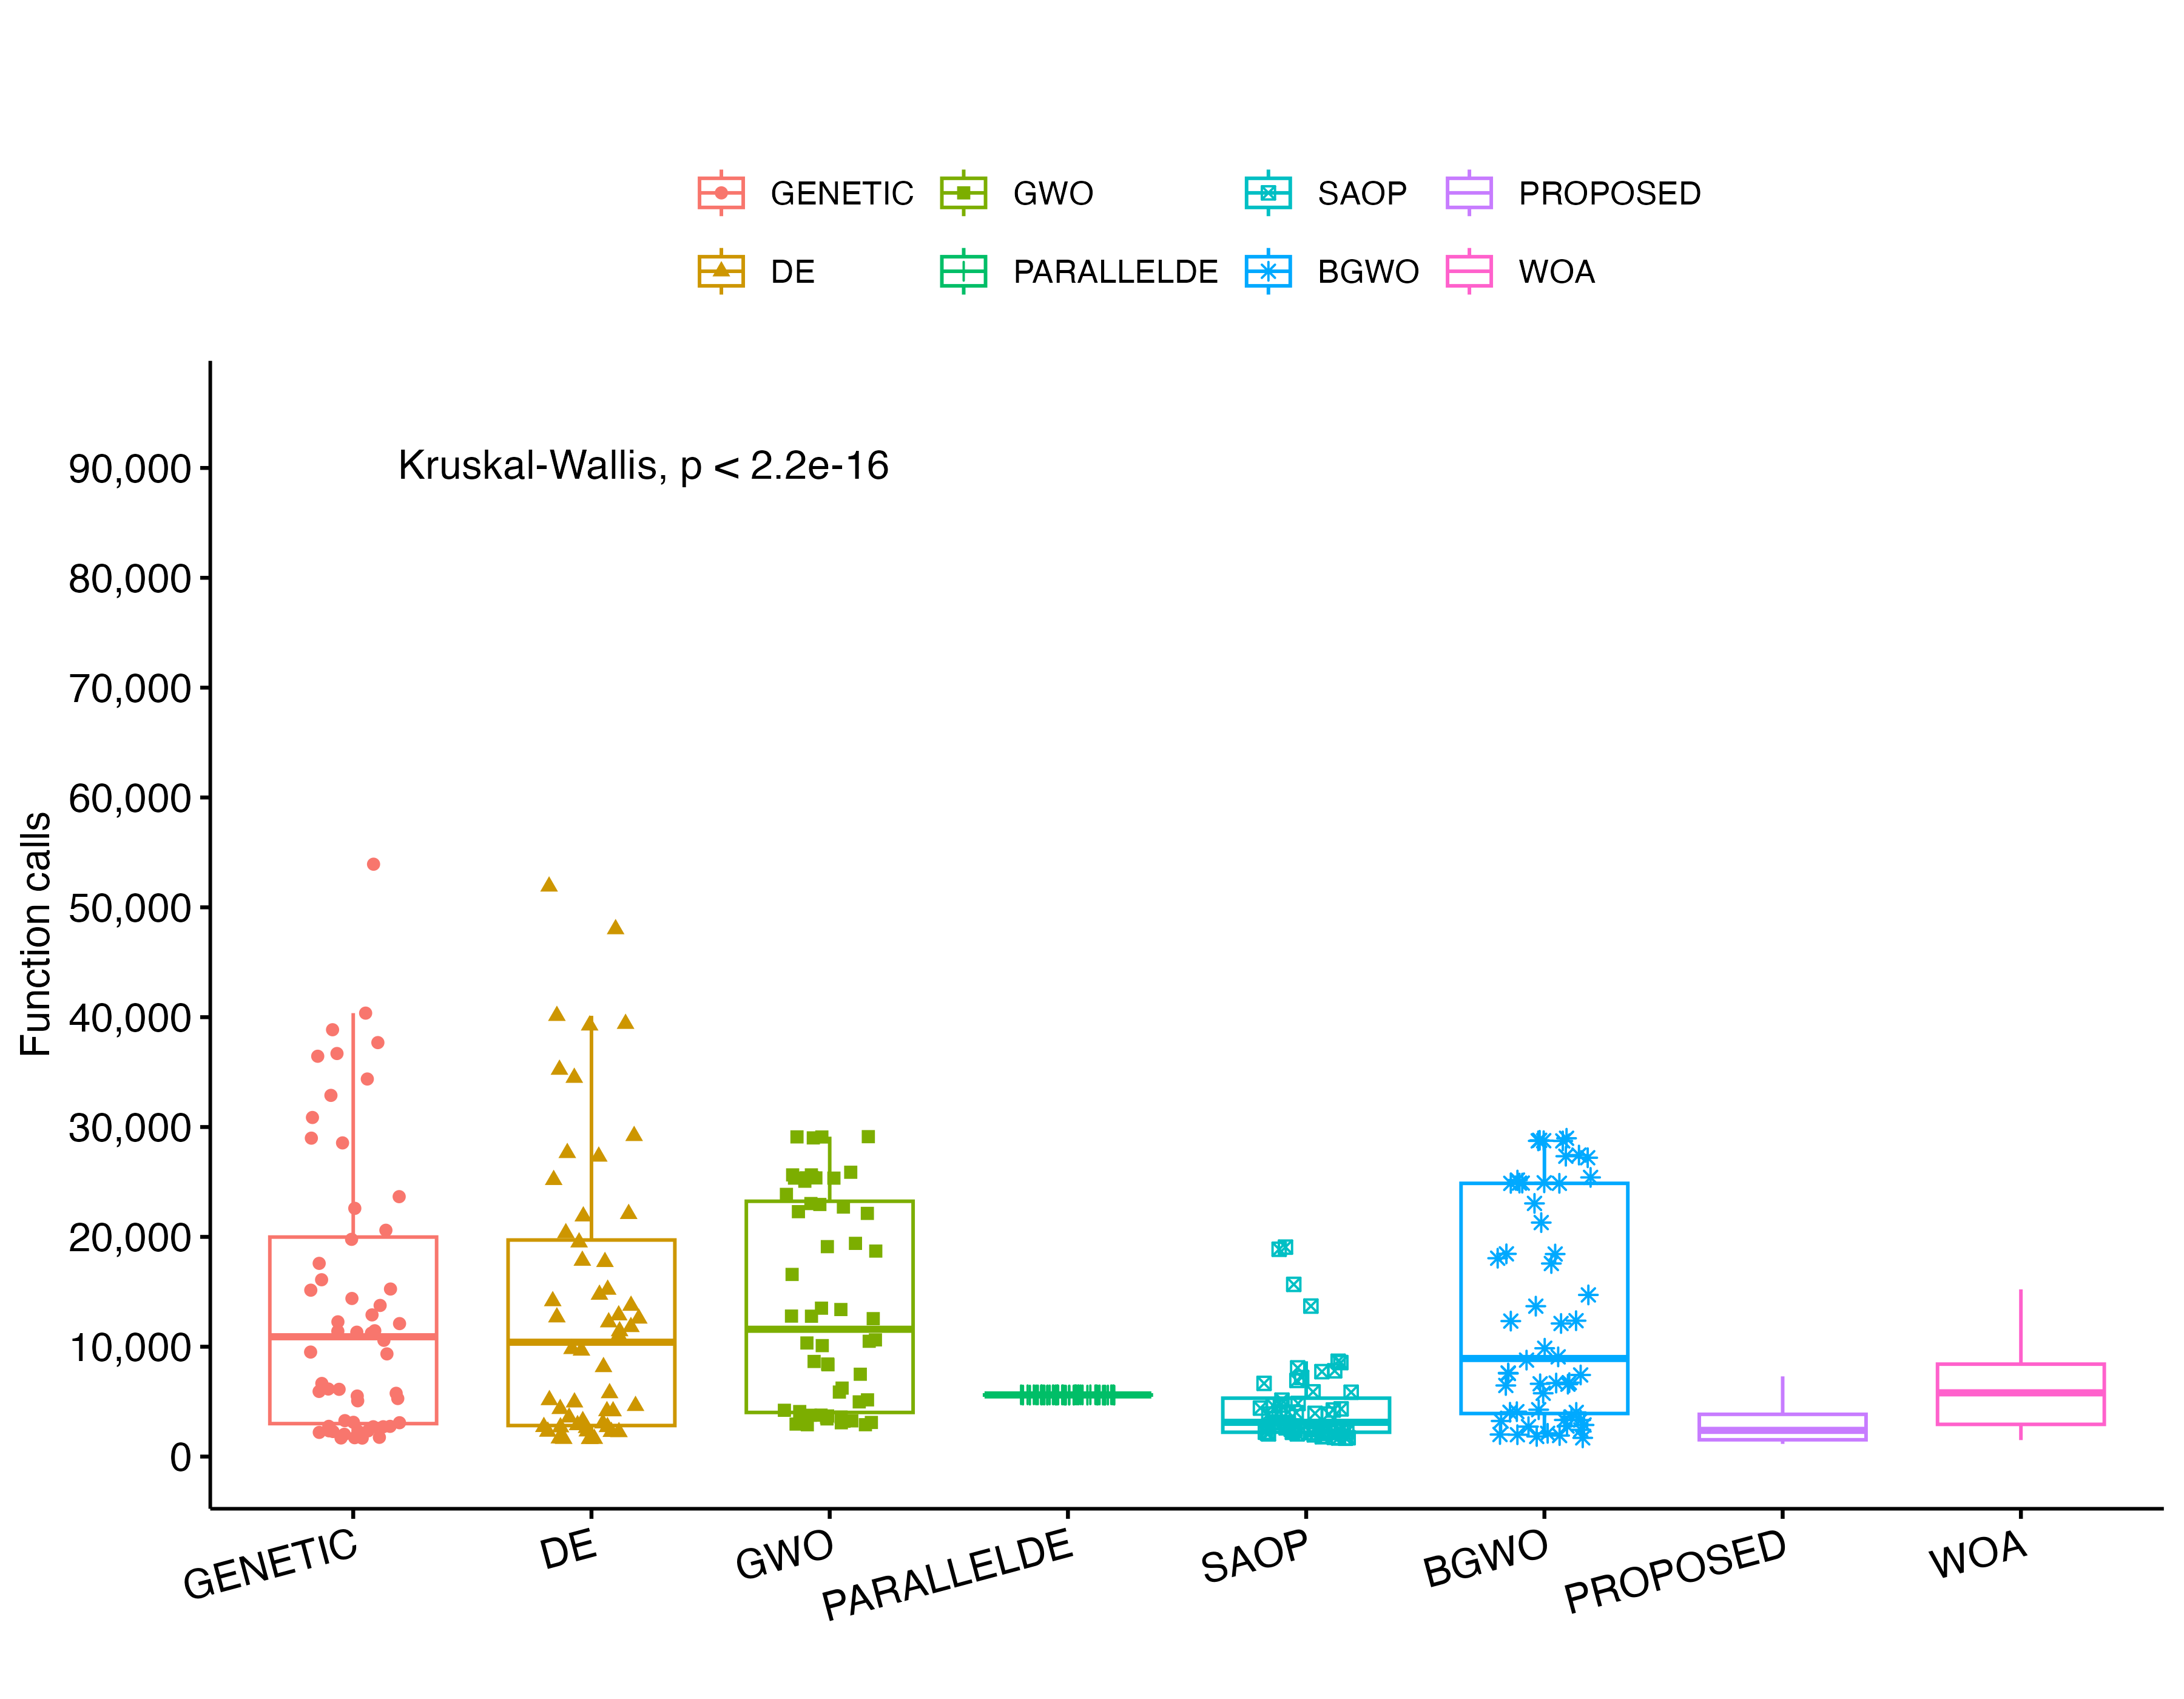
\includegraphics[scale=0.6]{Methods}\caption{The proposed method in comparison with others.\label{fig:The-proposed-method}}

\end{figure}

Figure \ref{fig:The-proposed-method} shows the comparison of the
performance of various optimization algorithms in terms of the number
of function calls. Specifically, the comparison of the algorithms
GENETIC, DE, GWO, PARALLELDE, SAOP, BGWO, PROPOSED and WOA. It is
observed that the proposed algorithm presents the smallest values
of function calls and less variance compared to most algorithms, therefore
it has faster convergence.The GENETIC, DE and BGWO algorithms show
greater dispersion and higher values, while PARALLELDE shows low values.
The Kruskal--Wallis statistical test (p \textless{} 2.2e\textminus 16)
shows that there are statistically significant differences between
the algorithms. Overall, the results indicate that the proposed method
is superior in terms of efficiency.

\subsection{Robust Statistical Evaluation of Algorithm Performance}

To provide a more rigorous and statistically sound evaluation of the
proposed method, the final optimization performance is assessed using
multiple statistical indicators. Specifically the results are reported
in terms of the mean and standard deviation (mean \textpm{} std) of
the final objective function values over 30 independent runs as summarized
in Table \ref{tab:Statistical-comparison-of}. The proposed method
consistently achieves near-zero objective values with negligible variance,
demonstrating both high accuracy and strong robustness compared to
the competing algorithms. In contrast, the majority of the compared
methods exhibit significantly higher objective values and larger variability,
indicating less stable performance. Overall these results highlight
the superiority of the proposed method in terms of both solution quality
and robustness across the examined benchmark functions.

\begin{table}
{\tiny{}%
\begin{tabular}{|c|c|c|c|c|c|c|c|c|}
\hline 
{\tiny Function} & {\tiny GA} & {\tiny DE} & {\tiny GWO} & {\tiny PARALLELDE} & {\tiny SAOP} & {\tiny BGWO} & {\tiny WOA} & {\tiny PROPOSED}\tabularnewline
\hline 
\hline 
{\tiny RASTRIGIN\_25} & {\tiny 4.84(18.12)} & {\tiny 5.07(19.08)} & {\tiny 2.35(8.81)} & {\tiny 0(0)} & {\tiny 5.37(20.37)} & {\tiny 1.69(6.87)} & {\tiny 3.34(18.03)} & {\tiny 0(0)}\tabularnewline
\hline 
{\tiny RASTRIGIN\_50} & {\tiny 42.61(49.41)} & \multirow{1}{*}{{\tiny 69.74(80.28)}} & {\tiny 2.58(7.66)} & {\tiny 0(0)} & {\tiny 47.32(55.60)} & {\tiny 25.76(35.22)} & {\tiny 37.57(53.86)} & {\tiny 1.49(5.65)}\tabularnewline
\hline 
{\tiny RASTRIGIN\_100} & {\tiny 90.40(60.40)} & {\tiny 184.99(123.56)} & {\tiny 20.33(48.36)} & {\tiny 0(0)} & {\tiny 106.29(73.03)} & {\tiny 51.67(35.30)} & {\tiny 22.65(57.87)} & {\tiny 1.55(8.39)}\tabularnewline
\hline 
{\tiny RASTRIGIN\_150} & {\tiny 111.56(93.76)} & {\tiny 216.70(178.74)} & {\tiny 34.29(71.21)} & {\tiny 0(0)} & {\tiny 126.39(105.46)} & {\tiny 72.69(66.19)} & {\tiny 6.79(36.61)} & {\tiny 0.63(3.39)}\tabularnewline
\hline 
\begin{cellvarwidth}[t]
\centering
{\tiny STEP}{\tiny\par}

{\tiny ELLIPSOIDAL\_25}
\end{cellvarwidth} & {\tiny 209.96(801.86)} & {\tiny 169.30(634.53)} & {\tiny 0(0)} & {\tiny 0(0)} & {\tiny 50.80(206.66)} & {\tiny 0(0)} & {\tiny 0(0)} & {\tiny 0(0)}\tabularnewline
\hline 
\begin{cellvarwidth}[t]
\centering
{\tiny STEP}{\tiny\par}

{\tiny ELLIPSOIDAL\_50}
\end{cellvarwidth} & {\tiny 2578.93(3001.44)} & {\tiny 2798.96(3259.50)} & {\tiny 0(0)} & {\tiny 0(0)} & {\tiny 1413.39(1665.82)} & {\tiny 0.29(0.97)} & {\tiny 0.50(2.20)} & {\tiny 0(0)}\tabularnewline
\hline 
\begin{cellvarwidth}[t]
\centering
{\tiny STEP}{\tiny\par}

{\tiny ELLIPSOIDAL\_100}
\end{cellvarwidth} & {\tiny 7265.83(4901.31)} & {\tiny 7331.79(4950.73)} & {\tiny 0.03(0.19)} & {\tiny 0(0)} & {\tiny 5816.37(3915.09)} & {\tiny 1.74(2.79)} & {\tiny 0.58(3.13)} & {\tiny 0(0)}\tabularnewline
\hline 
\begin{cellvarwidth}[t]
\centering
{\tiny STEP}{\tiny\par}

{\tiny ELLIPSOIDAL\_150}
\end{cellvarwidth} & {\tiny 7842.70(6466.45)} & {\tiny 7842.70(6466.45)} & {\tiny 0.48(2.61)} & {\tiny 0(0)} & {\tiny 7344.09(6055.11)} & {\tiny 2.58(3.29)} & {\tiny 0.22(1.20)} & {\tiny 0(0)}\tabularnewline
\hline 
\end{tabular}}{\tiny\par}

\caption{Statistical comparison of optimization algorithms on benchmark functions
in terms of mean and standard deviation (mean \textpm{} std) of the
final objective values over 30 independent runs. \label{tab:Statistical-comparison-of}}
\end{table}


\subsection{Performance comparison on low-dimensional benchmark functions}

To further strengthen the experimental evaluation, a subset of standard
benchmark functions commonly used in deterministic global optimization
is considered, including both GKLS instances and classical low-dimensional
test functions such as\textbf{ }BRANIN, GOLDSTEIN and HARTMAN \citep{key-3,key-4}.
Specifically these problems correspond to low-dimensional settings
providing a suitable testbed for assessing performance in scenarios
where deterministic methods are particularly effective, as summarized
in Table \ref{tab:Performance-comparison-of} The proposed method
consistently requires significantly fewer function evaluations to
reach the target accuracy across all tested instances. In particular,
it achieves substantial reductions in computational effort compared
to the other considered methods, often exceeding 50\%. These results
demonstrate the efficiency and robustness of the proposed approach
in low-dimensional deterministic optimization problems.

\begin{table}
{\scriptsize{}%
\begin{tabular}{|c|c|c|c|c|c|c|c|c|c|}
\hline 
{\scriptsize Function} & {\scriptsize DIMENSION} & {\scriptsize GA} & {\scriptsize DE} & {\scriptsize GWO} & {\scriptsize PARALLELDE} & {\scriptsize SAOP} & {\scriptsize BGWO} & {\scriptsize WOA} & {\scriptsize PROPOSED}\tabularnewline
\hline 
\hline 
{\scriptsize BRANIN} & {\scriptsize 2} & {\scriptsize 2017} & {\scriptsize 1940} & {\scriptsize 3325} & {\scriptsize 6547} & {\scriptsize 2123} & {\scriptsize 3118} & {\scriptsize 2297} & {\scriptsize 570}\tabularnewline
\hline 
{\scriptsize GKLS250} & {\scriptsize 2} & {\scriptsize 1806} & {\scriptsize 1754} & {\scriptsize 3668} & {\scriptsize 6478} & {\scriptsize 1468} & {\scriptsize 3009} & {\scriptsize 2016} & {\scriptsize 547}\tabularnewline
\hline 
{\scriptsize GKLS350} & {\scriptsize 3} & {\scriptsize 1761} & {\scriptsize 1711} & {\scriptsize 3691} & {\scriptsize 10454} & {\scriptsize 1352(0.97)} & {\scriptsize 3178} & {\scriptsize 2366(0.87)} & {\scriptsize 507}\tabularnewline
\hline 
{\scriptsize GOLDSTEIN} & {\scriptsize 2} & {\scriptsize 2792} & {\scriptsize 2676} & {\scriptsize 5376} & {\scriptsize 6888} & {\scriptsize 3149} & {\scriptsize 3794} & {\scriptsize 2470} & {\scriptsize 750}\tabularnewline
\hline 
{\scriptsize HARTMAN} & {\scriptsize 3} & {\scriptsize 2109} & {\scriptsize 2062} & {\scriptsize 3222} & {\scriptsize 7828} & {\scriptsize 1646} & {\scriptsize 2790} & {\scriptsize 2640} & {\scriptsize 575}\tabularnewline
\hline 
\end{tabular}}{\scriptsize\par}

\caption{Performance comparison of optimization algorithms on low-dimensional
benchmark functions reported in terms of the number of function evaluations
required to reach the target accuracy. \label{tab:Performance-comparison-of}}
\end{table}


\subsection{Performance Comparison Between DIRECT and the Proposed Method}

Based on the results presented in Table\textbf{ }\ref{tab:Number of objective function evaluations for DIRECT and the proposed method. }
where the values correspond to the number of objective function evaluations,
the performance of the proposed method relative to DIRECT varies \citep{key-7}
across benchmark functions and problem dimensions. For the Zakharov
function, the proposed method consistently requires significantly
fewer evaluations across all tested dimensions (100, 150 and 200)
indicating a clear efficiency advantage. In the AttractiveSector function
the performance is mixed: the proposed method is less efficient at
100 dimensions, comparable at 150 dimensions and more efficient at
200 dimensions. Similarly, for the Step Ellipsoidal function, the
proposed method requires more evaluations at lower dimensions (100
and 150) but outperforms DIRECT at 200 dimensions. Overall, while
DIRECT exhibits stable performance due to its deterministic nature
the proposed method demonstrates improved efficiency in higher-dimensional
cases, suggesting a more effective handling of increased problem complexity.

{\scriptsize{}
\begin{table}[H]
{\scriptsize\caption{Number of objective function evaluations for DIRECT and the proposed
method. \label{tab:Number of objective function evaluations for DIRECT and the proposed method. }}
}{\scriptsize\par}
\centering{}{\small{}%
\begin{tabular}{|c|c|c|}
\hline 
{\small\textbf{FUNCTION}} & DIRECT & PROPOSED\tabularnewline
\hline 
\hline 
\begin{cellvarwidth}[t]
\centering
{\small ATTRACTIVE}{\small\par}

{\small SECTOR\_100}
\end{cellvarwidth} & 1198 & {\small 1818}\tabularnewline
\hline 
\begin{cellvarwidth}[t]
\centering
{\small ATTRACTIVE}{\small\par}

{\small SECTOR\_150}
\end{cellvarwidth} & 1798 & {\small 1754}\tabularnewline
\hline 
\begin{cellvarwidth}[t]
\centering
{\small ATTRACTIVE}{\small\par}

{\small SECTOR\_200}
\end{cellvarwidth} & 2398 & 1562\tabularnewline
\hline 
{\small STEP\_ELLIPSOIDAL\_100} & 1000 & {\small 1737}\tabularnewline
\hline 
{\small STEP ELLIPSOIDAL\_150} & 1500 & {\small 1698}\tabularnewline
\hline 
{\small STEP ELLIPSOIDAL\_200} & 2000 & 1497\tabularnewline
\hline 
{\small ZAKHAROV\_100} & 10182 & {\small 1344}\tabularnewline
\hline 
{\small ZAKHAROV\_150} & 12257 & {\small 1539}\tabularnewline
\hline 
{\small ZAKHAROV\_200} & 12278 & 1276\tabularnewline
\hline 
\end{tabular}}{\small\par}
\end{table}
}{\scriptsize\par}

\subsection{A sensitivity analysis}

A sensitivity analysis is conducted to assess the impact of the propagation
parameters $N_{R}$ and $N_{P}$ on the performance of the proposed
algorithm using the Rosenbrock function ($D$ = 25). The results expressed
in terms of the number of function evaluations, are presented in Figures
\ref{fig:A sensitivity analysis_NR} and \ref{fig:A sensitivity analysis_NP}.
As illustrated in Figure 8, the parameter $N_{R}$ has a significant
influence on the computational cost. In particular, increasing $N_{R}$
generally results in a higher number of function evaluations, although
the relationship is not strictly monotonic. This behavior suggests
that larger propagation ranges enhance exploration capabilities, at
the expense of increased computational overhead due to redundant evaluations.
In contrast Figure 9 shows that the parameter $N_{P}$ has a relatively
limited effect on the number of function evaluations, as only minor
variations are observed across different parameter settings. Overall
moderate values of both parameters appear to provide an effective
trade-off between convergence efficiency and computational cost. Furthermore
the communication cost increases with higher values of $N_{R}$ and
$N_{P}$ since broader propagation mechanisms lead to more frequent
interactions among agents. Notably the solution quality remains largely
stable across different parameter configurations indicating that the
proposed algorithm is robust with respect to $N_{R}$ and $N_{P}$.
This observation suggests that these parameters primarily influence
computational effort rather than the final optimization accuracy.

\begin{figure}
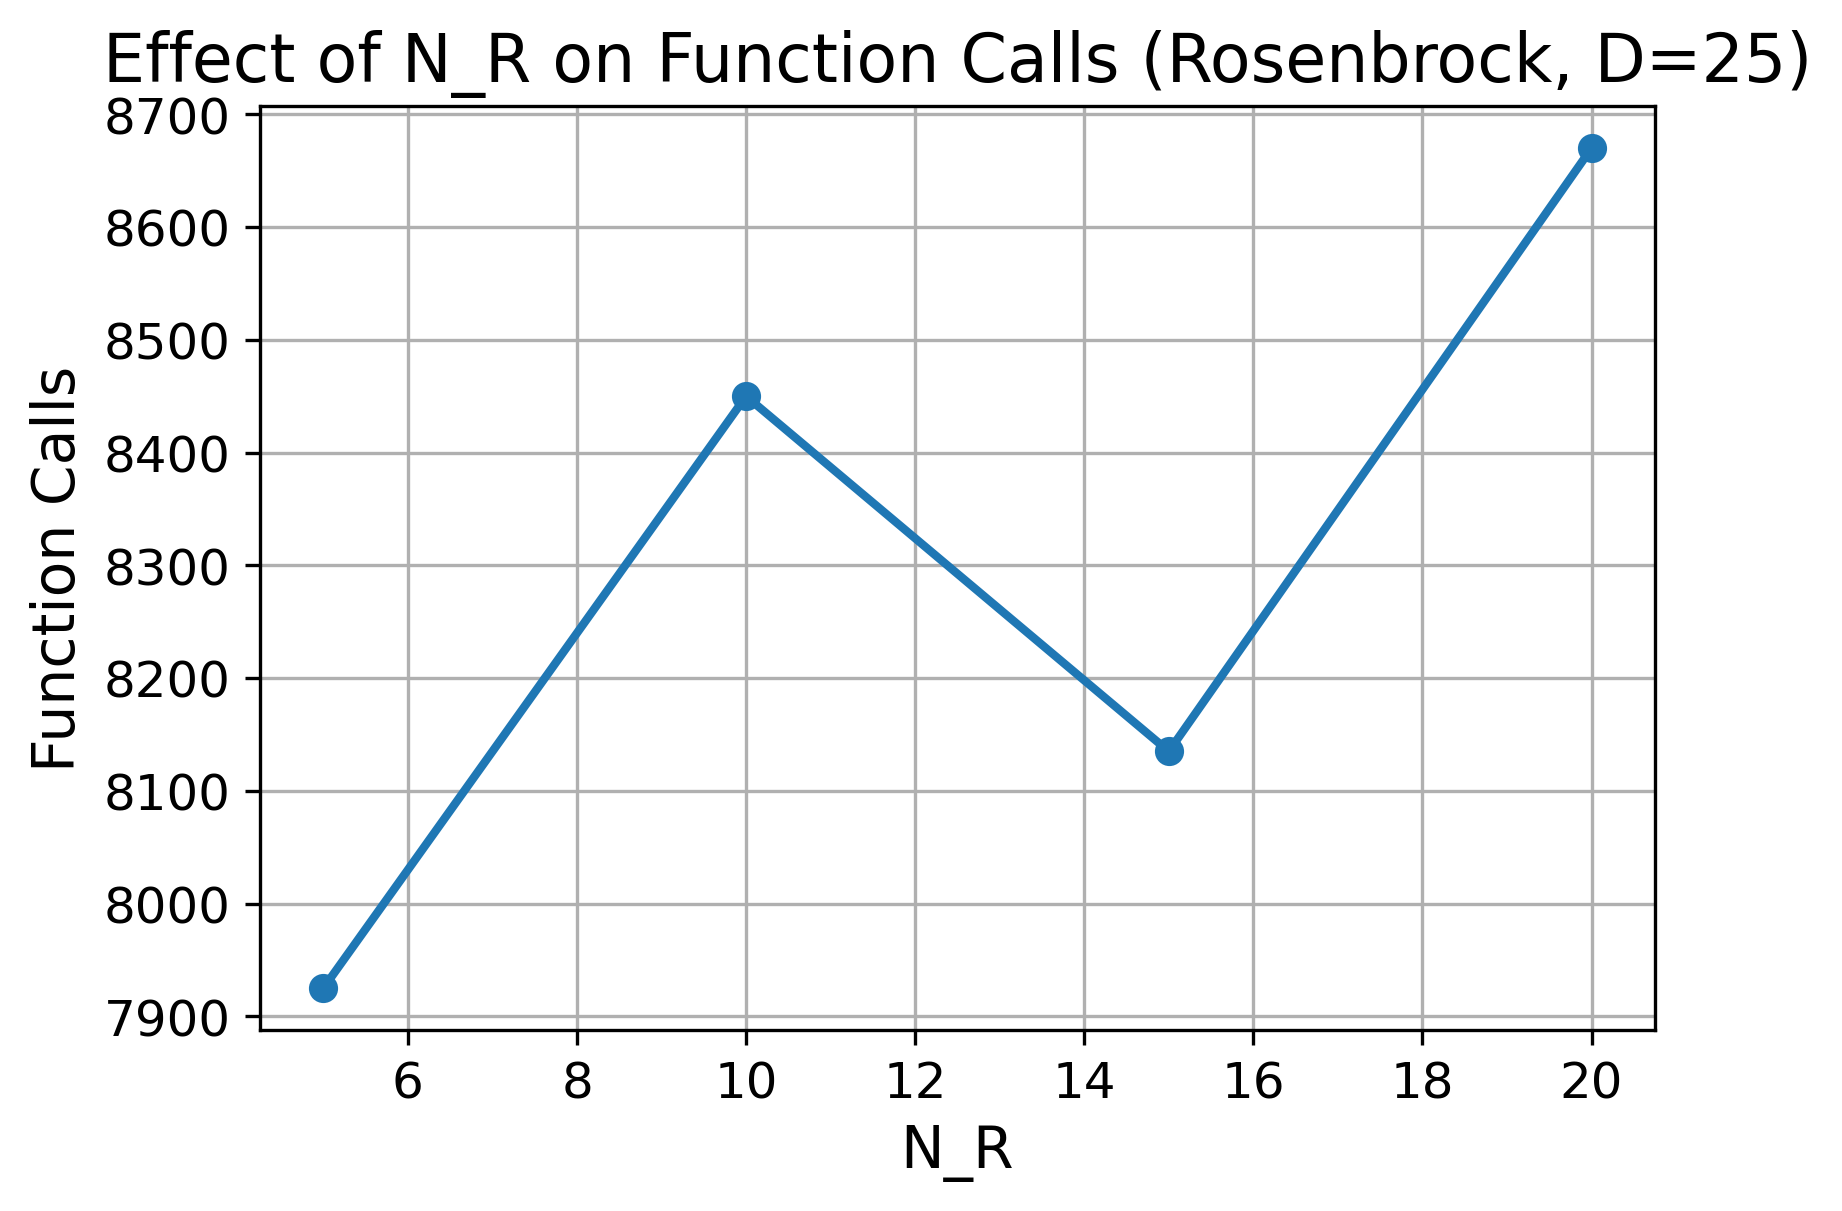
\includegraphics[scale=0.75]{NR}

\caption{Sensitivity analysis of the propagation parameter $N_{R}$ in terms
of the number of function evaluations on the Rosenbrock function (D
= 25). \label{fig:A sensitivity analysis_NR}}
\end{figure}

\begin{figure}
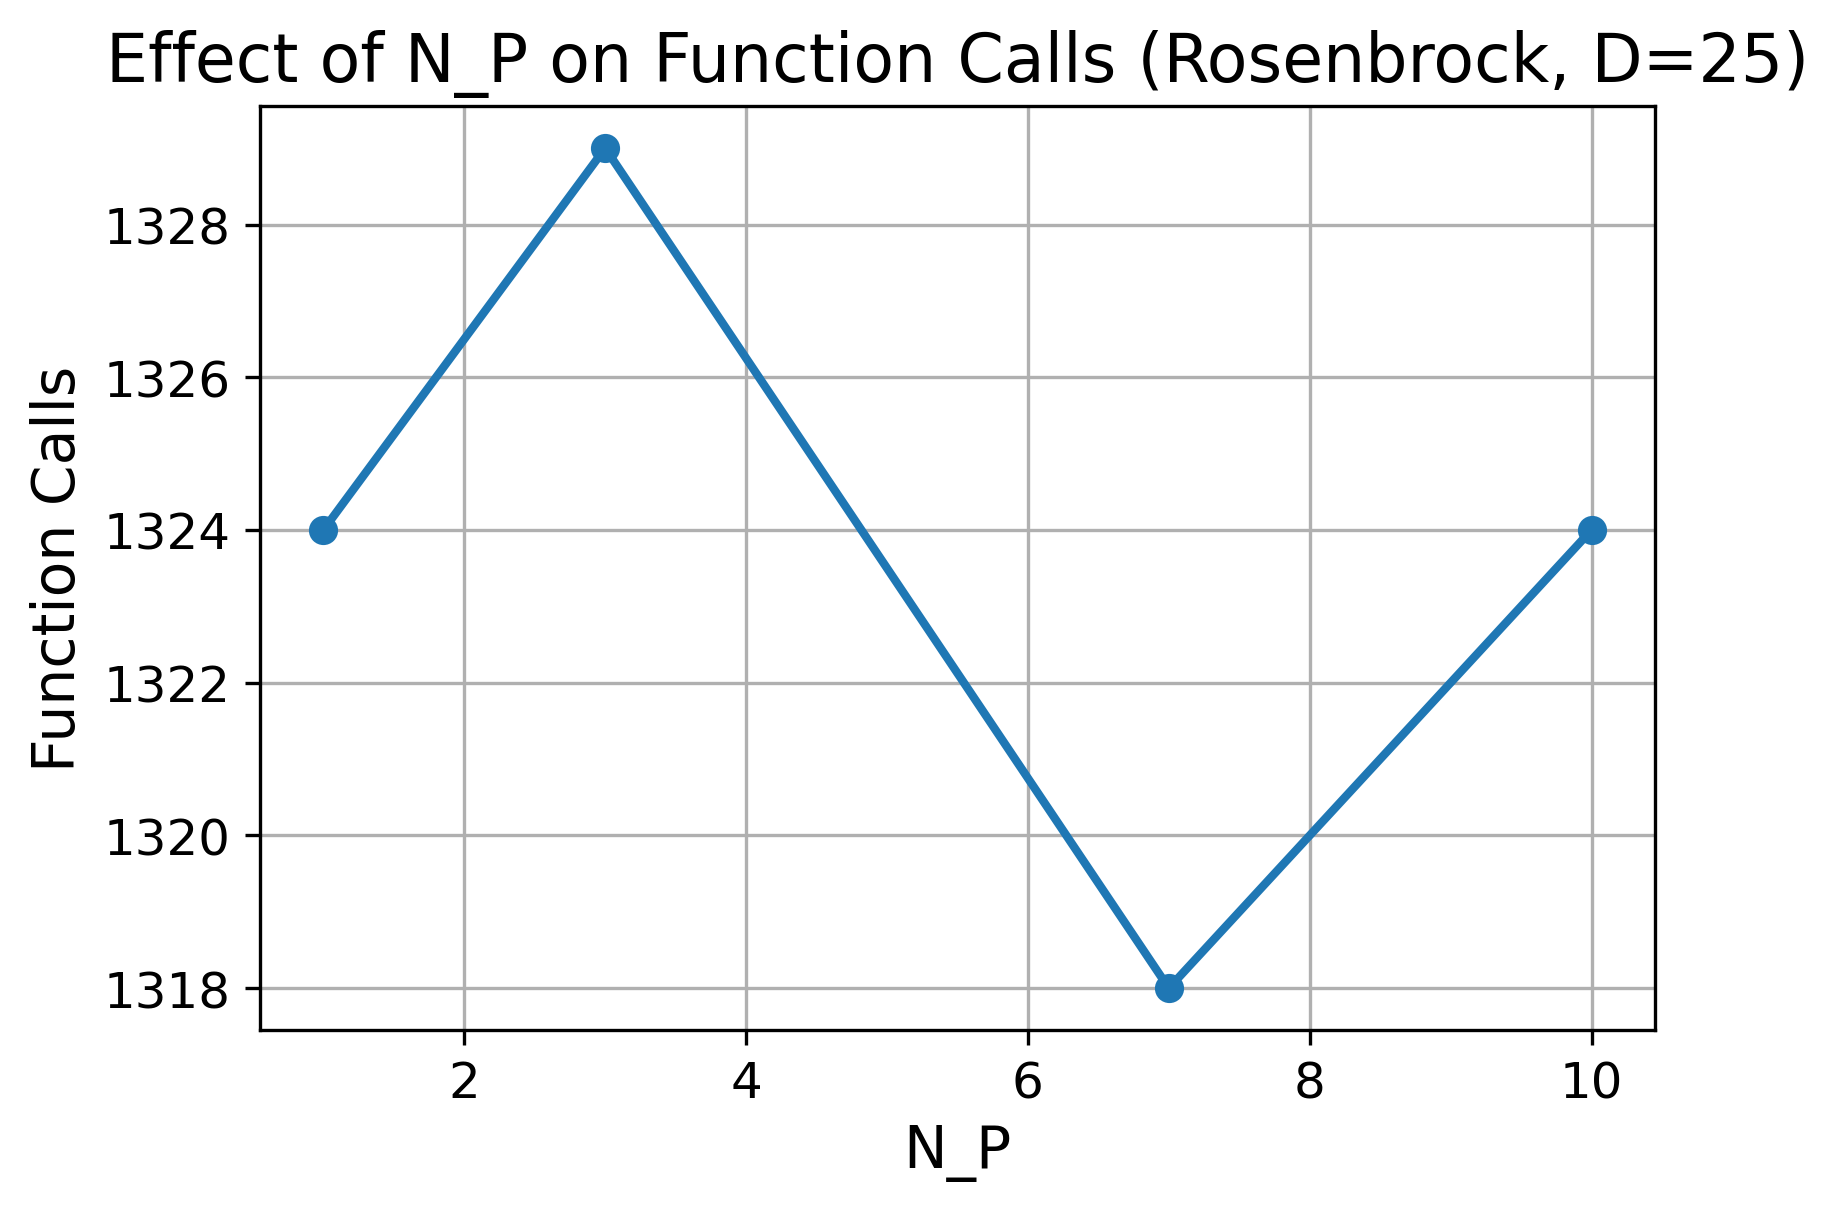
\includegraphics[scale=0.75]{NP}\caption{Sensitivity analysis of the propagation parameter $N_{P}$ in terms
of the number of function evaluations on the Rosenbrock function (D
= 25). \label{fig:A sensitivity analysis_NP}}
\end{figure}

To further investigate the effect of information exchange mechanisms,
a sensitivity analysis of the four propagation strategies (1to1, 1toN,
Nto1 and NtoN) is conducted under varying values of the propagation
parameters $N_{R}$ and $N_{P}$. The corresponding results are presented
in Figures \ref{fig:A sensitivity analysis_NR_prop} and \ref{fig:A sensitivity analysis_NP_prop}
. As illustrated in Figure 10, the choice of propagation strategy
has a pronounced impact on convergence behavior. In particular, the
NtoN strategy achieves the lowest number of function evaluations for
smaller values of $N_{R}$, indicating accelerated convergence due
to intensive information exchange. However, as $N_{R}$ increases
the performance of NtoN deteriorates, suggesting that excessive propagation
may introduce redundant communication and reduce overall efficiency.
In contrast, more localized strategies, such as 1to1 exhibit more
stable behavior across different values of $N_{R}$ albeit with generally
slower convergence. The 1toN and Nto1 strategies demonstrate intermediate
performance, effectively balancing exploration and exploitation. Figure
11 further highlights the influence of the propagation strategies
with respect to $N_{P}$. Specifically the NtoN strategy consistently
attains the lowest number of function evaluations demonstrating significantly
faster convergence. This observation indicates that frequent and widespread
information exchange can substantially accelerate the optimization
process. Nevertheless such aggressive propagation schemes may lead
to premature homogenization of the population whereby diversity is
rapidly reduced and the algorithm becomes prone to convergence to
suboptimal solutions. Conversely more restrictive strategies preserve
population diversity for longer periods, resulting in slower yet potentially
more robust convergence. Overall, the propagation strategy introduces
a trade-off between convergence speed, communication cost and population
diversity. Moderate interaction schemes (such as 1toN and Nto1) provide
a balanced compromise achieving efficient convergence while mitigating
the risk of premature homogenization.

\begin{figure}
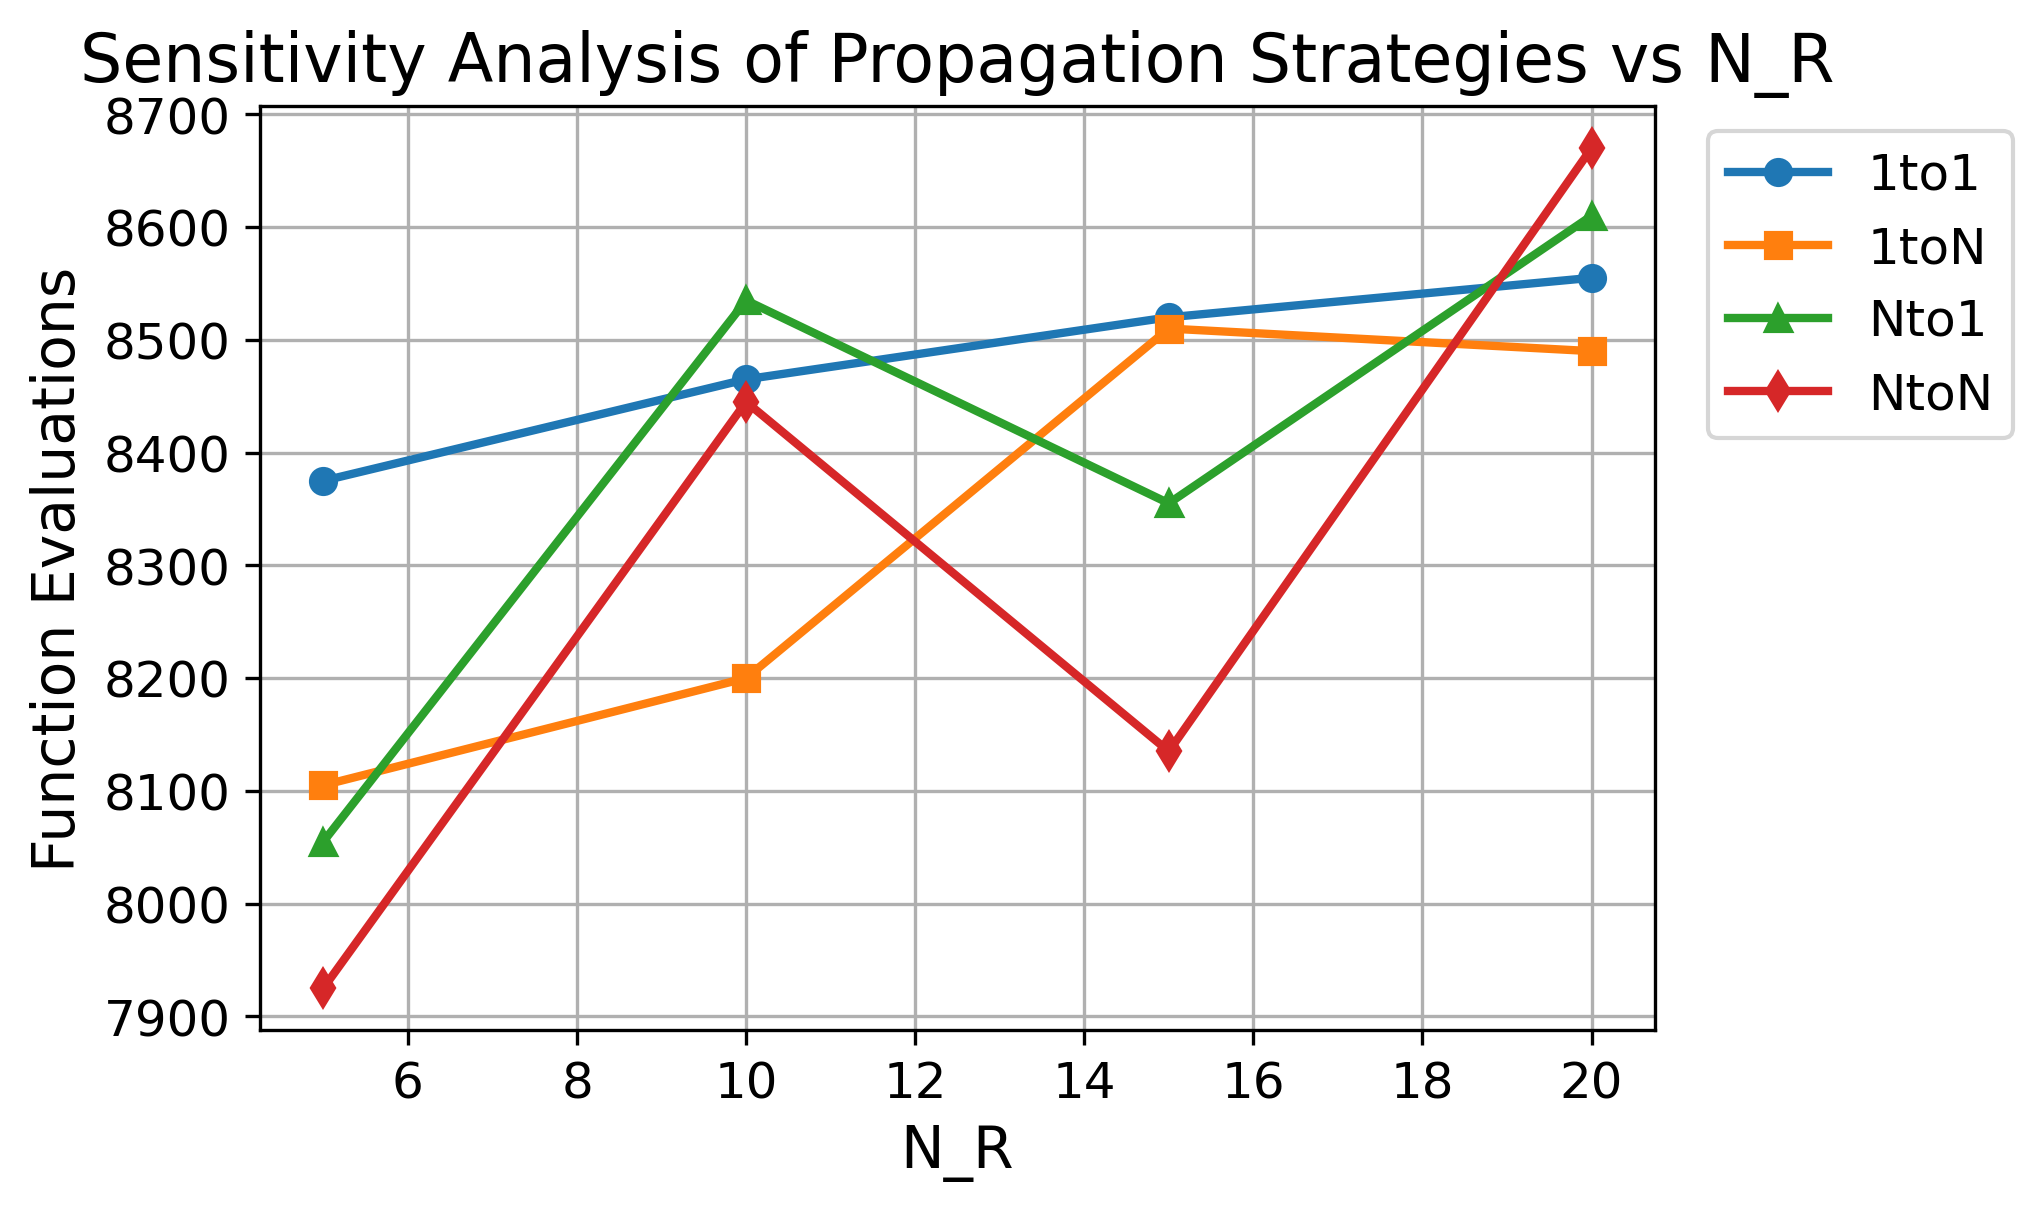
\includegraphics[scale=0.75]{prop_NR}\caption{Effect of different propagation strategies (1to1, 1toN, Nto1, NtoN)
on convergence performance under varying values of $N_{R}$. \label{fig:A sensitivity analysis_NR_prop}}
\end{figure}

\begin{figure}
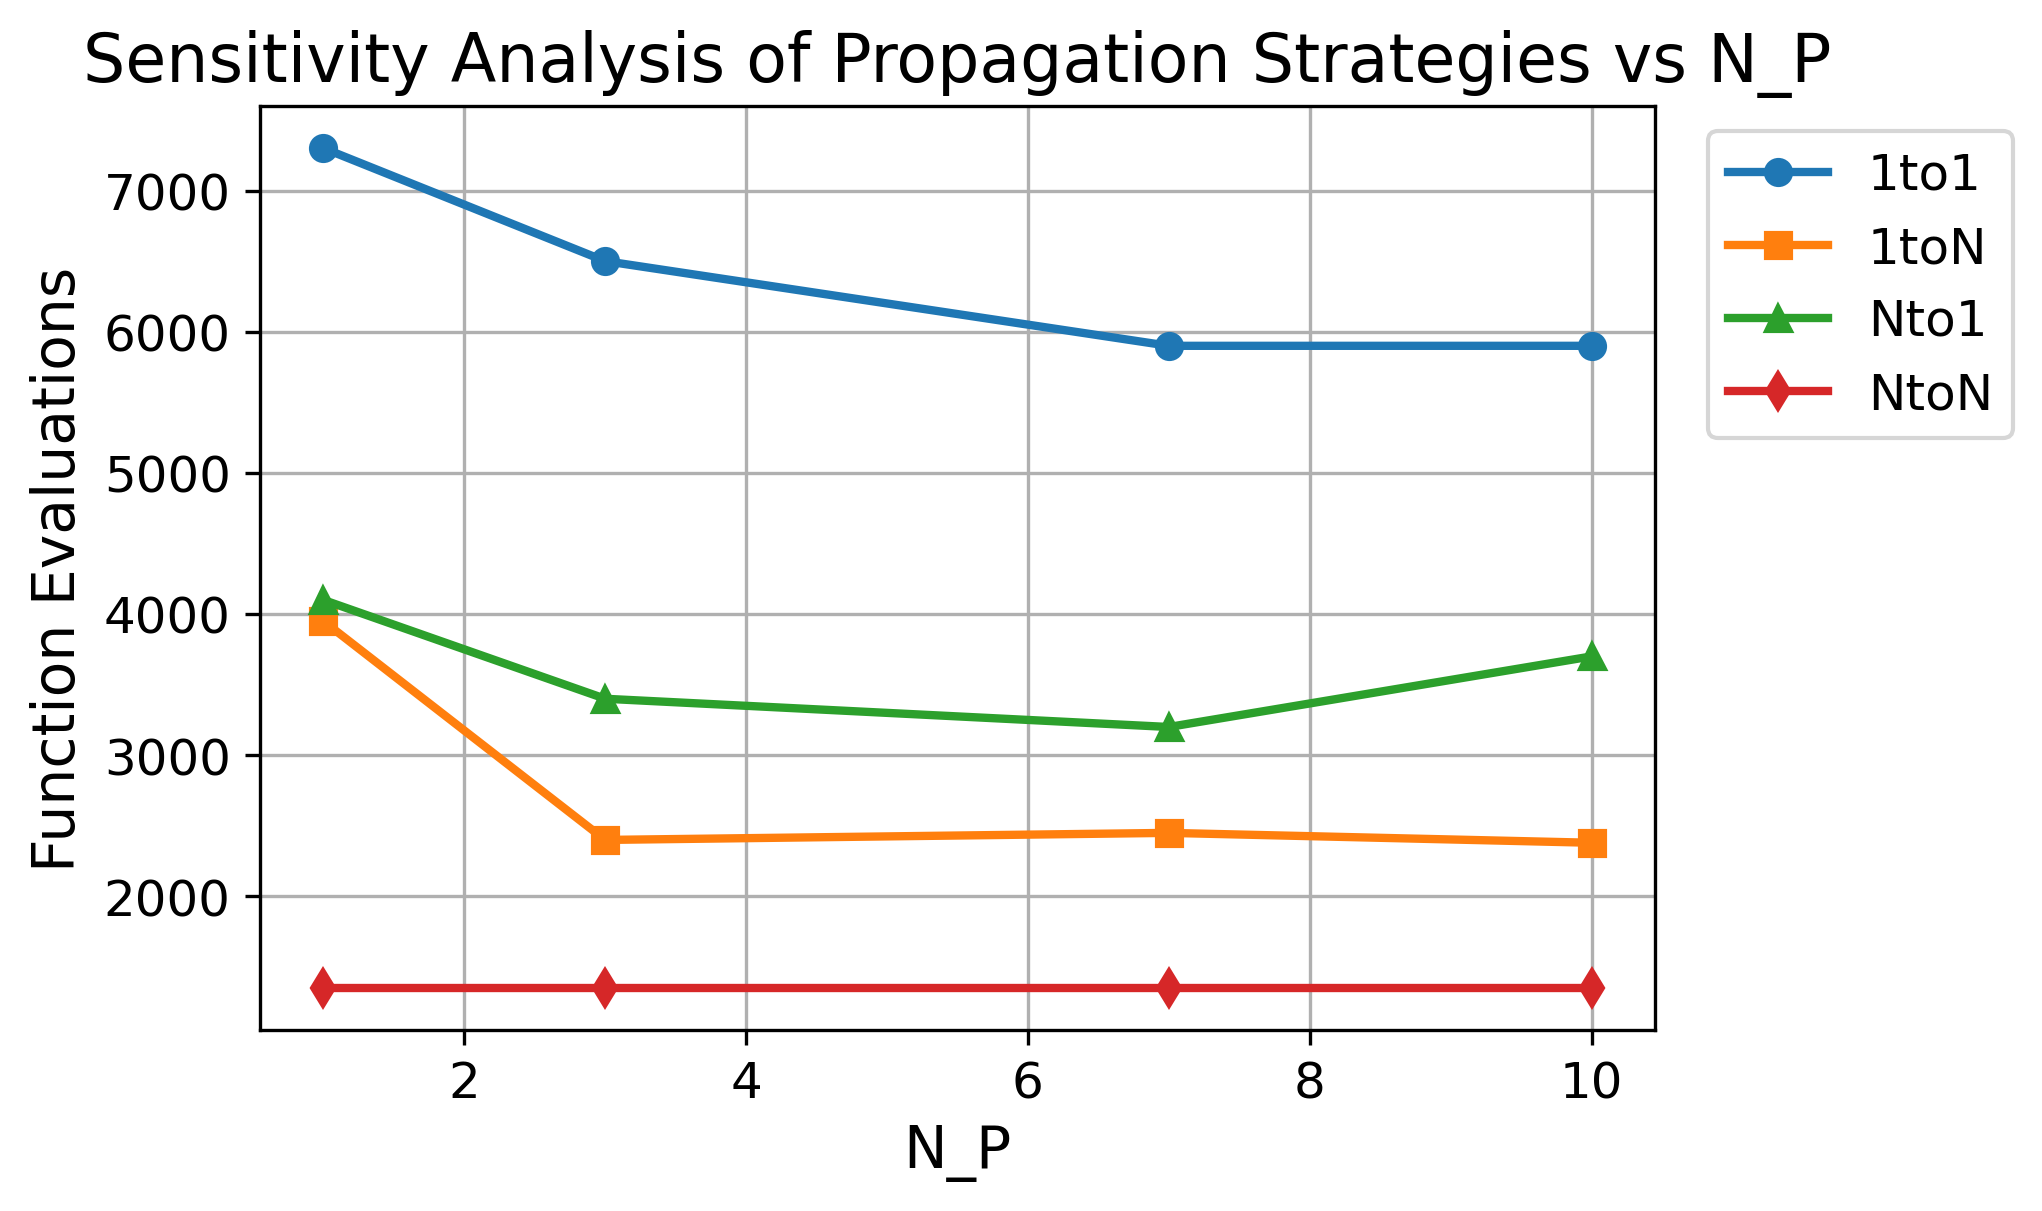
\includegraphics[scale=0.75]{prop_NP}

\caption{Effect of different propagation strategies (1to1, 1toN, Nto1, NtoN)
on convergence performance under varying values of $N_{P}$. \label{fig:A sensitivity analysis_NP_prop}}

\end{figure}


\subsection{Practical problems}

To further examine the practical efficiency and scalability of the
proposed optimization algorithm, two real-world engineering design
problems were investigated: the GasCycle \citep{GasCycle} and the
Tandem Queueing System \citep{Tandem}. These problems were selected
because they differ significantly in mathematical formulation and
computational complexity, providing a comprehensive framework for
evaluating the algorithm’s performance under diverse and realistic
conditions.

Each problem was tested across multiple dimensional configurations,
ranging from 25 to 500 variables, in order to assess how the algorithm
behaves as the search space becomes more complex. For every configuration,
the execution time in seconds was recorded as the main performance
indicator. This experimental setup enables a direct comparison of
how computational efficiency changes with increasing dimensionality.
\begin{itemize}
\item \textbf{GasCycle Thermal Cycle}

Vars: $\bm{x}=[T_{1},T_{3},P_{1},P_{3}]^{\top}$. \quad{}$r=P_{3}/P_{1},\ \gamma=1.4.$
\[
\eta(\bm{x})=1-r^{-(\gamma-1)/\gamma}\,\frac{T_{1}}{T_{3}},\qquad\min_{\bm{x}}f(\bm{x})=-\eta(\bm{x}).
\]
Bounds: $300\!\le\!T_{1}\!\le\!1500,\;1200\!\le\!T_{3}\!\le\!2000,\;1\!\le\!P_{1},P_{3}\!\le\!20.$

Penalty: infeasible $\Rightarrow f=10^{20}$.

The GasCycle scenario presents a more computationally demanding optimization
problem, allowing a clearer assessment of algorithmic scalability
under increased complexity.

\begin{figure}

\includegraphics[scale=0.65]{GasCycle1}\caption{Comparison of Function Calls Across Dimensions (GasCycle).\label{fig:Comparison-of-Function}}

\end{figure}

\end{itemize}
Figure \ref{fig:Comparison-of-Function} outlines the comparison of
the number of calls of the objective function with respect to the
dimension of the problem for the GasCycle problem. It is observed
that most methods generally show a constant or slightly decreasing
trend in the number of function calls as the dimension increases.
The PARALLELDE algorithm maintains a significantly higher number of
calls in all dimensions. GENETIC, GWO, BGWO and DE move in medium
value levels, presenting mild fluctuations. The proposed method (ParallelBGWO)
displays one of the lowest values in the number of calls and maintains
a relatively constant and controllable behavior throughout the range
of dimensions.

\begin{figure}

\includegraphics[scale=0.75]{Gascycle_time}\caption{Comparison of Execution Time Across Dimensions (GasCycle).\label{fig:Comparison-of-Execution}}

\end{figure}

Figure \ref{fig:Comparison-of-Execution} shows the comparison of
the execution time of the algorithms with respect to the dimension
of the problem for the GasCycle problem. It is observed that the execution
time increases progressively with increasing dimension for all methods,
which is expected due to the increased computational complexity. PARALLELDE
shows significantly longer execution times compared to the other algorithms.
GENETIC, GWO, BGWO, SAOP, DE and WOA show a similar scaling with a
relatively smooth and linear increase in time. The proposed method
(ParallelBGWO) follows a corresponding incremental path maintaining
execution times comparable to most algorithms of the same category
and clearly lower than PARALLELDE.
\begin{itemize}
\item \textbf{Tandem Space Trajectory} (MGA-1DSM, EVEEJ + 2$\times$Saturn)

{\footnotesize Vars}{\footnotesize\textbf{ ($D{=}18$):}}{\footnotesize{}
$\bm{x}=[t_{0},T_{1},T_{2},T_{3},T_{4},T_{5A},T_{5B},s_{1},s_{2},s_{3},s_{4},s_{5A},s_{5B},r_{p},k_{A1},k_{A2},k_{B1},k_{B2}]^{\top}$.
\[
\begin{aligned} & 7000\le t_{0}\le10000,\\
 & 30\le T_{1}\le500,\;30\le T_{2}\le600,\;30\le T_{3}\le1200,\\
 & 30\le T_{4}\le1600,\;30\le T_{5A},T_{5B}\le2000,\\
 & 0\le s_{1..4},s_{5A},s_{5B},r_{p},k_{A1},k_{A2},k_{B1},k_{B2}\le1.
\end{aligned}
\]
}{\footnotesize\par}

{\footnotesize Objective: 
\[
\min_{\bm{x}}\ \Delta V_{\text{tot}}=\Delta V_{\text{launch}}(T_{1})+\Delta V_{\text{legs}}(T_{1}{:}T_{4})+\Delta V_{A}+\Delta V_{B}+\Delta V_{\text{DSM}}(\bm{s},r_{p})-G_{\text{GA}}-G_{J}+P_{\text{hard}}+P_{\text{soft}},
\]
\medskip{}
 
\[
P_{\text{soft}}=\beta\max\!\Big\{0,\ (T_{1}{+}\cdots{+}T_{4}+\tfrac{1}{2}(T_{5A}{+}T_{5B}))-3500\Big\}.
\]
Notes: $\Delta V_{\text{launch}}$ decreases (log-like) in $T_{1}$
($\ge6$ km/s floor), leg/branch costs decrease with TOF.}{\footnotesize\par}

\medskip{}

\end{itemize}
\begin{figure}

\includegraphics[scale=0.65]{Tandem1}

\caption{Comparison of Function Calls Across Dimensions (Tandem).\label{fig:Comparison-of-Function-1}}

\end{figure}

Figure \ref{fig:Comparison-of-Function-1} shows the comparison of
the number of calls of the objective function with respect to the
dimension of the problem for the algorithms under consideration. It
is observed that the number of function calls remains relatively constant
for most methods as the dimension increases, with small fluctuations
per case. The BGWO algorithm displays the highest number of calls
in almost all dimensions, maintaining high values with small changes.
GENETIC and PARALLELDE exhibit greater fluctuations. In contrast GWO,
SAOP, DE and WOA move at lower call levels with relatively smooth
behavior. The proposed method (ParallelBGWO) exhibits among the lowest
values in the number of calls and maintains a stable behavior as the
dimension increases.

\begin{figure}

\includegraphics[scale=0.75]{Tandem_time}

\caption{Comparison of Execution Time Across Dimensions (Tandem).\label{fig:Comparison-of-Execution-1}}

\end{figure}

Figure \ref{fig:Comparison-of-Execution-1} shows the comparison of
the execution time of various algorithms with respect to the dimension
of the problem. We observe that as the dimension increases, the execution
time for all algorithms also increases. The proposed method (ParallelBGWO)
clearly exhibits better scaling behavior compared to the classic BGWO
and other algorithms, maintaining lower execution times in all dimensions
especially in large dimensions (400--500). In contrast, algorithms
such as Genetic and ParallelDE show a sharp increase in execution
time in high dimensions which indicates lower computational efficiency
on large problems. Overall the results demonstrate that the proposed
ParallelBGWO achieves a better balance between performance and computational
cost making it a suitable choice for large-scale problems.

\subsection{Comprehensive Evaluation of Solution Quality and Efficiency on Real-World
Problems}

Table \ref{tab:Final-solution-quality} presents the final solution
quality obtained by all compared algorithms on the GasCycle and Tandem
case studies. The results are reported in terms of the mean and standard
deviation over 30 independent runs. As observed all algorithms achieve
comparable objective values particularly for the GasCycle problems,
where the solutions converge to nearly identical values with negligible
variance. This indicates that the considered problems can be reliably
solved by multiple methods. Notably the proposed method attains solution
quality that is on par with the best-performing algorithms without
any observable degradation in accuracy. These findings confirm that
the previously demonstrated reductions in function evaluations and
execution time are not achieved at the expense of solution quality.
Moreover, the low standard deviation values across most cases indicate
stable and consistent performance. Overall, the results demonstrate
that the proposed approach effectively balances computational efficiency
and solution accuracy in real-world optimization scenarios. Furthermore
it is important to note that both the GasCycle and Tandem case studies
correspond to well-defined optimization problems in which all candidate
solutions remain feasible by construction. Consequently constraint
violations are not applicable and all methods consistently produce
feasible solutions.

\begin{table}
{\tiny{}%
\begin{tabular}{|c|c|c|c|c|c|c|c|c|}
\hline 
{\tiny Function} & {\tiny GA} & {\tiny DE} & {\tiny GWO} & {\tiny PARALLELDE} & {\tiny SAOP} & {\tiny BGWO} & {\tiny WOA} & {\tiny PROPOSED}\tabularnewline
\hline 
\hline 
{\tiny Tandem\_50} & {\tiny 27.72(0.16)} & {\tiny 27.83(0.19)} & {\tiny 28(2.42)} & {\tiny 28.24(0.33)} & {\tiny 28.69(0.67)} & {\tiny 27.84(0.18)} & {\tiny 28.96(0.68)} & {\tiny 28.16(0.34)}\tabularnewline
\hline 
{\tiny Tandem\_100} & {\tiny 27.67(0.10)} & {\tiny 27.80(0.14)} & {\tiny 28.64(2.00)} & {\tiny 28.19(0.29)} & {\tiny 28.80(0.76)} & {\tiny 27.85(0.25)} & {\tiny 29.04(0.66)} & {\tiny 28.20(0.39)}\tabularnewline
\hline 
{\tiny Tandem\_200} & {\tiny 27.66(0.11)} & {\tiny 27.87(0.21)} & {\tiny 28.11(2.23)} & {\tiny 28.25(0.30)} & {\tiny 28.72(0.56)} & {\tiny 27.81(0.16)} & {\tiny 28.99(0.68)} & {\tiny 28.26(0.37)}\tabularnewline
\hline 
{\tiny GasCycle\_50} & {\tiny -0.93($9.75\times10^{-10}$)} & {\tiny -0.93($8.67\times10^{-10}$)} & {\tiny -0.93(0)} & {\tiny -0.93(0)} & {\tiny -0.93(0.17)} & {\tiny -0.93(0)} & {\tiny -0.92(0.01)} & {\tiny -0.9(0.01)}\tabularnewline
\hline 
{\tiny GasCycle\_100} & {\tiny -0.93($8.01\times10^{-10})$} & {\tiny -0.93($1.16\times10^{-9}$)} & {\tiny -0.93(0)} & {\tiny -0.93(0)} & {\tiny -0.91(0.16)} & {\tiny -0.93(0)} & {\tiny -0.92(0.01)} & {\tiny -0.9(0.01)}\tabularnewline
\hline 
{\tiny GasCycle\_200} & {\tiny -0.93($1.30\times10^{-9}$)} & {\tiny -0.93($3.43\times10^{-9}$)} & {\tiny -0.93(0)} & {\tiny -0.93(0)} & {\tiny -0.92(0.012)} & {\tiny -0.93(0)} & {\tiny -0.92(0.01)} & {\tiny -0.9(0.013)}\tabularnewline
\hline 
\end{tabular}}{\tiny\par}

\caption{Final solution quality obtained by all compared algorithms on the
GasCycle and Tandem case studies, reported as mean and standard deviation
(mean \textpm{} std) over 30 independent runs. \label{tab:Final-solution-quality}}
\end{table}


\subsection{Impact of the Subpopulation Termination Criterion on Practical Problems}

Figure \ref{fig:Effect-of-SubPopulation} shows the effect of different
subpopulation termination criteria (ANY, MAJORITY, ALL) on the number
of objective function evaluations for the GasCycle problem in different
dimensions. From the results, it is observed that the ANY strategy
presents the smallest number of function calls in all dimensions.
This shows that a more flexible termination criterion can significantly
reduce the computational cost. In contrast, the MAJORITY strategy
requires a larger number of evaluations as termination is triggered
only when the majority of subpopulations are completed. The ALL strategy
displays the highest values since it requires the completion of all
subpopulations before termination. Therefore the results show that
the more stringent the termination criterion the higher the overall
computational cost.

\begin{figure}

\includegraphics[scale=0.65]{GasCycle}

\caption{Effect of SubPopulation Termination Rule on Function Evaluations (GasCycle).\label{fig:Effect-of-SubPopulation}}

\end{figure}

In the Tandem problem, a similar behavior is observed regarding the
effect of the termination criteria on the number of evaluations of
the objective function. The ANY strategy also presents the lowest
function calls values in all dimensions, thus it is a more flexible
termination criterion that can significantly reduce the computational
cost. The MAJORITY strategy presents greater variability and generally
requires more evaluations, while the ALL strategy leads to the largest
function calls values, as the search process continues until all subpopulations
are completed.\textbf{ }Therefore, the stringency of the termination
criterion significantly affects the efficiency of the algorithm, with
the ANY strategy offering the most computationally efficient approach.
This improvement in computational efficiency is achieved without any
noticeable degradation in solution quality as confirmed by the results
reported in Table 13. The final objective values obtained using the
ANY strategy remain comparable to those achieved with the MAJORITY
and ALL strategies. The experimental results for this case are shown
graphically in Figure \ref{fig:Effect-of-SubPopulation-1}.

\begin{figure}

\includegraphics[scale=0.65]{Tandem}

\caption{Effect of SubPopulation Termination Rule on Function Evaluations (Tandem).\label{fig:Effect-of-SubPopulation-1}}

\end{figure}

Table \ref{tab:Comparison-of-final} reports the mean and standard
deviation of the final objective values obtained by the ANY, MAJORITY
and ALL strategies for the Tandem and GasCycle case studies across
different problem sizes. The mean values correspond to the average
performance over multiple independent runs, while the standard deviation
reflects the consistency and robustness of each strategy. The results
indicate that all three strategies achieve comparable objective values
across all cases, with only minor differences observed. In addition,
the relatively low standard deviation values suggest stable performance
across runs for all strategies. In conjunction with the results presented
in Figures 16 and 17, which show a reduction in the number of function
evaluations for the ANY strategy, these findings suggest that the
improvement in computational efficiency is not accompanied by a significant
change in final solution quality. Overall, the ANY, MAJORITY and ALL
strategies demonstrate similar levels of solution quality, with ANY
offering improved efficiency while maintaining comparable performance.

\begin{table}
\begin{tabular}{|c|c|c|c|}
\hline 
Function & ANY & MAJORITY & ALL\tabularnewline
\hline 
\hline 
Tandem\_25 & 28.22(0.35) & 28.12(0.45) & 27.99(0.35)\tabularnewline
\hline 
Tandem\_50 & 28.20(0.39) & 28.05(0.37) & 28.04(0.44)\tabularnewline
\hline 
Tandem\_100 & 28.26(0.37) & 27.97(0.44) & 27.99(0.32)\tabularnewline
\hline 
Tandem\_150 & 28.21(0.36) & 28.09(0.43) & 28.10(0.36)\tabularnewline
\hline 
GasCycle\_25 & -0.91(0.011) & -0.92(0.008) & -0.92(0.010)\tabularnewline
\hline 
GasCycle\_50 & -0.91(0.018) & -0.92(0.013) & -0.92(0.016)\tabularnewline
\hline 
GasCycle\_100 & -0.90(0.013) & -0.92(0.011) & -0.92(0.008)\tabularnewline
\hline 
GasCycle\_150 & -0.91(0.013) & -0.91(0.02) & -0.92(0.008)\tabularnewline
\hline 
\end{tabular}

\caption{Comparison of final objective values (mean \textpm{} standard deviation)
for the ANY, MAJORITY and ALL strategies on Tandem and GasCycle Practical
Problems. \label{tab:Comparison-of-final}}
\end{table}


\subsection{Neural Network Training Experiments}

To validate the effectiveness of the proposed method, it was applied
to the training of artificial neural networks \citep{nn1,nn2} for
classification problems using benchmark datasets from publicly available
repositories.

The neural network training experiments were conducted using a Multilayer
Perceptron (MLP) architecture with a single hidden layer consisting
of 10 neurons. The network weights were initialized within the range
{[}-10, 10{]}. The evaluation was performed on classification datasets
obtained from the UCI Machine Learning Repository using a ten-fold
cross-validation protocol. All input features were normalized prior
to training. The training objective was defined as the minimization
of the Mean Squared Error (MSE). The optimization process follows
a hybrid global--local strategy. In the global phase, the ParallelBGWO
is employed with a population of 50 agents, distributed across subpopulations
during parallel execution (1, 5 and 10 threads). The propagation mechanism
$N_{M}$ is set to the Nto1 communication scheme, enabling controlled
information exchange among subpopulations. In the local phase, the
BFGS algorithm is applied for 200 iterations to refine the best solution
obtained from the global search. The optimization process is terminated
using a similarity-based stopping criterion.

The classification datasets were selected from widely used benchmark
repositories, including the UCI Machine Learning Repository the KEEL
dataset repository and the StatLib database. These datasets were chosen
due to their diversity in dimensionality, class distribution, and
classification complexity allowing for a comprehensive evaluation
of the performance and robustness of the proposed optimization method.
Results are reported as the mean classification error over multiple
independent runs.
\begin{enumerate}
\item The UCI database, \url{https://archive.ics.uci.edu/}(accessed on
28 March 2026)\citep{uci}
\item The Keel website, \url{https://sci2s.ugr.es/keel/datasets.php}(accessed
on 28 March 2026)\citep{Keel}.
\item The Statlib URL \url{https://lib.stat.cmu.edu/datasets/index}(accessed
on 28 March 2026).
\end{enumerate}
From these databases the following datasets were obtained:
\begin{enumerate}
\item \textbf{Circular} dataset, that contains artificially generated data.
\item \textbf{Heart} dataset \citep{heart} a medical dataset used for the
prediction of heart diseases.
\item \textbf{Ionosphere} dataset, a climate dataset \citep{ion1,ion2}.
\item \textbf{Liverdisorder} dataset \citep{liver} a medical dataset.
\item \textbf{Lymography} dataset\citep{lymography}.
\item \textbf{Pima} dataset \citep{pima}.
\item \textbf{Spiral} dataset, which is an artificial dataset.
\item \textbf{Statheart}, a dataset related to the detection of heart diseases.
\item \textbf{Wdbc} dataset \citep{wdbc}.
\item \textbf{Wine} dataset, used for the detection of quality of wines
\citep{wine1,wine2}.
\end{enumerate}
All experiments were conducted 10 times, each with a different random
seed. To validate the results, the widely used ten-fold cross-validation
method was applied. For the classification datasets, the mean classification
error is presented, computed according to the following formula:
\begin{equation}
E_{C}\left(N\left(\overrightarrow{x},\overrightarrow{w}\right)\right)=100\times\frac{\sum_{i=1}^{N}\left(\mbox{class}\left(N\left(\overrightarrow{x_{i}},\overrightarrow{w}\right)\right)-y_{i}\right)}{N}
\end{equation}
In this equation, the set $T$ denotes the used test set. In the experiments
the following methods was used:
\begin{enumerate}
\item ADAM optimizer \citep{nn_adam} is used to train a neural network
with 10 processing nodes.
\item BFGS optimizer was incorporated to train a neural network with 10
processing nodes.
\item GENETIC, where a neural network \citep{Genetic,Genetic-1} was used
to train a neural network with 10 processing nodes.
\item PROPOSED, where the described method is used to train a neural network
with 10 processing nodes.
\end{enumerate}
The selected classification datasets are widely used benchmark problems
in the machine learning and neural network literature, enabling reliable
evaluation of classification performance. Furthermore they provide
diversity in terms of dimensionality class distribution and classification
complexity allowing for a comprehensive assessment of the effectiveness
and robustness of the proposed optimization method across different
types of learning tasks. In addition, these datasets correspond to
optimization problems of varying difficulty in neural network training,
including high-dimensional and non-convex search spaces. This makes
them suitable for evaluating the performance of the proposed method
in large-scale black-box optimization settings.

The results obtained by the previously mention methods are presented
in Table \ref{tab:experClass}.

\begin{table}[H]
\caption{Average Classification Error Rates on some classification datasets
using a series of methods.\label{tab:experClass}}

\centering{}%
\begin{tabular}{|c|c|c|c|c|}
\hline 
\textbf{DATASET} & \textbf{ADAM} & \textbf{BFGS} & \textbf{GENETIC} & \textbf{PROPOSED}\tabularnewline
\hline 
\hline 
Circular & 19.95\% & 6.08\% & 5.99\% & 4.30\%\tabularnewline
\hline 
Heart & 38.53\% & 39.44\% & 28.34\% & 18.17\%\tabularnewline
\hline 
Ionosphere & 16.64\% & 15.29\% & 15.14\% & 15.00\%\tabularnewline
\hline 
Liverdisorder & 41.53\% & 42.59\% & 31.11\% & 32.89\%\tabularnewline
\hline 
Lymography & 39.79\% & 35.43\% & 28.42\% & 24.60\%\tabularnewline
\hline 
Pima & 34.85\% & 35.59\% & 32.19\% & 25.25\%\tabularnewline
\hline 
Spiral & 47.67\% & 47.99\% & 48.66\% & 41.80\%\tabularnewline
\hline 
Statheart & 44.04\% & 39.65\% & 27.25\% & 20.62\%\tabularnewline
\hline 
Wine & 29.40\% & 59.71\% & 19.20\% & 11.24\%\tabularnewline
\hline 
Wdbc & 35.35\% & 29.91\% & 8.56\% & 4.50\%\tabularnewline
\hline 
\textbf{AVERAGE} & \textbf{34.78\%} & \textbf{35.17\%} & \textbf{26.26\%} & \textbf{19.84\%}\tabularnewline
\hline 
\end{tabular}
\end{table}

Table \ref{tab:experClass} indicates that PROPOSED is the most effective
method overall in terms of classification error rate, since it achieves
the lowest average error, 19.84\% compared with 26.26\% for GENETIC,
34.78\% for ADAM and 35.17\% for BFGS. Because lower values correspond
to better performance, this result demonstrates a clear overall superiority
of PROPOSED over both the two gradient-based baselines and the evolutionary
GENETIC approach. This advantage is not marginal but substantial,
suggesting that the proposed scheme attains a more favorable balance
between adaptation and generalization across the examined classification
datasets.

At the individual dataset level, PROPOSED ranks first in 9 out of
the 10 datasets, yielding the lowest error on Circular, Heart, Ionosphere,
Lymography, Pima, Spiral, Statheart, Wine and Wdbc. The only exception
is Liverdisorder, where GENETIC achieves a slightly lower error rate
than PROPOSED. Nevertheless this isolated case does not alter the
overall pattern, which is characterized by consistent and widespread
superiority of the proposed method across heterogeneous classification
problems. It is particularly noteworthy that the advantage of PROPOSED
is preserved even on demanding datasets such as Spiral, while especially
pronounced improvements are observed on Heart, Statheart, Wine and
Wdbc relative to the competing methods.

Overall, the results support the conclusion that PROPOSED does not
merely provide occasional strong outcomes, but rather exhibits greater
robustness and stronger generalization ability across nearly the entire
experimental setting. Therefore it can be regarded as the most reliable
method among the four compared models under the present evaluation
protocol. Results are reported as the mean classification error over
multiple independent runs.

\begin{figure}[H]
\begin{centering}

\includegraphics[scale=0.65]{stat_tbl8}
\par\end{centering}
\caption{Statistical comparison of ANN training methods based on Friedman/Nemenyi
post-hoc analysis \label{fig:stat_tbl8}}
\end{figure}

The statistical analysis based on the Friedman test with Nemenyi post-hoc
procedure showed that there are overall statistically significant
differences among the four models on the classification datasets of
Table \ref{tab:experClass}. Specifically the overall Friedman p-value
is $5.28\times10^{-5}$, which is well below 0.05, thus rejecting
the null hypothesis of equivalent model performance in terms of classification
error.

The pairwise comparisons reported in Figure \ref{fig:stat_tbl8} indicate
that PROPOSED significantly outperforms both ADAM and BFGS, since
in both cases the obtained p-value is $3.95\times10^{-4}$ corresponding
to an extremely significant difference. In contrast, the comparisons
ADAM-BFGS (p = 1.0000), ADAM-GENETIC (p = 0.1096), BFGS-GENETIC (p
= 0.1096) and GENETIC-PROPOSED (p = 0.3069) are not statistically
significant at the $\alpha$ = 0.05 level. Therefore, the results
establish PROPOSED as the statistically strongest approach relative
to the classical ADAM and BFGS schemes, whereas its superiority over
GENETIC, although visible at the level of average error, is not statistically
confirmed by the Nemenyi post-hoc test.

\section{Discussion\label{sec:Discussion}}

\subsection{Effect of the Parallel Architecture}

The experimental results demonstrate that the effectiveness of ParallelBGWO
derives from the coordinated integration of four principal structural
components: population partitioning into cooperating subpopulations,
inter-cluster information propagation, communication strategy selection,
and flexible termination criteria. Collectively, these mechanisms
improve the balance between exploration and exploitation, which is
fundamental in large-scale optimization. Furthermore, the findings
indicate that parallelization contributes not only to reduced execution
time but also to enhanced search dynamics since the concurrent exploration
of multiple search regions mitigates premature convergence and facilitates
the dissemination of beneficial search information. The analysis of
the number of subpopulations further indicates that algorithmic performance
is highly dependent on the degree of population partitioning. While
the transition from a single-population model to multiple cooperating
clusters significantly reduces computational cost, the improvement
is not monotonic. Specifically, configurations employing 10 and 20
subpopulations provide the most favorable trade-off whereas increasing
the number to 30 does not yield proportional benefits. This suggests
that excessive fragmentation may weaken the internal evolutionary
pressure of each subpopulation and reduce exploitation efficiency.
Consequently, an appropriate compromise between diversity preservation
and local search pressure is necessary. Overall, these findings suggest
that the effectiveness of the parallel architecture is strongly dependent
on maintaining a balance between subpopulation diversity and intra-cluster
selection pressure. While increasing the number of subpopulations
enhances exploration through distributed search, excessive fragmentation
weakens convergence pressure, leading to diminishing returns. This
highlights the importance of selecting an appropriate level of parallelism
depending on the problem complexity.

\subsection{Impact of Communication and Propagation Mechanisms}

The propagation mechanism is shown to constitute a critical component
of the proposed method. The comparison between PROP = 0 and PROP =
1 demonstrates that enabling information propagation significantly
decreases the number of objective function evaluations, indicating
that subpopulation cooperation is essential to the efficiency of the
optimization process. This finding suggests that the rapid dissemination
of locally generated high-quality solutions enhances the global guidance
of the search process. Similarly, the evaluation of alternative communication
strategies indicates that the fully bidirectional NtoN scheme consistently
achieves the lowest computational cost relative to the 1to1, 1toN
and Nto1 approaches. This superiority is further validated through
Friedman and Wilcoxon statistical tests, confirming that full information
exchange among subpopulations represents the most effective strategy
for exploiting cooperative parallelism. These observations reveal
a fundamental trade-off between communication intensity and population
diversity. While frequent and global information exchange (NtoN) accelerates
convergence by rapidly disseminating high-quality solutions, it also
increases the risk of premature convergence due to loss of diversity.
Conversely, more restrictive communication schemes preserve diversity
but slow down convergence. Therefore, selecting an appropriate propagation
strategy is crucial and should be adapted to the problem landscape.

\subsection{Analysis of Termination Strategies}

With respect to subpopulation termination criteria, the ANY strategy
consistently yields the lowest number of function evaluations on the
GasCycle and Tandem problems, whereas the MAJORITY and ALL strategies
result in higher computational cost. This outcome is expected, as
stricter termination rules prolong execution even when a subset of
subpopulations has already converged. These observations indicate
that termination flexibility constitutes a significant determinant
of algorithmic efficiency rather than a minor implementation detail.
The proposed framework benefits when unnecessary waiting among subpopulations
is minimized thereby allowing more efficient use of computational
resources.

\subsection{Comparative Performance Evaluation}

The comparison with established metaheuristic methods further reinforces
the effectiveness of the proposed approach. Across benchmark problems
with dimensionality ranging from 25 to 150, ParallelBGWO achieves
the lowest number of function evaluations compared with GA, DE, GWO,
ParallelDE, SAOP, BGWO and WOA. Its superiority is particularly evident
on demanding functions such as Zakharov and Sharp Ridge. Moreover,
in the practical GasCycle and Tandem optimization problems, ParallelBGWO
maintains low computational cost and execution time as dimensionality
increases thereby demonstrating improved scalability. This property
is particularly desirable in large-scale optimization contexts, where
the growth of computational burden must remain controlled as problem
complexity increases. While the proposed method demonstrates clear
advantages in terms of computational efficiency, a comprehensive evaluation
must also consider solution quality. The experimental results show
that the proposed approach consistently achieves competitive or superior
final objective values, accompanied by low standard deviation across
independent runs. This indicates not only high accuracy but also stable
and reliable convergence behavior. Therefore, the method improves
computational efficiency without compromising solution quality, achieving
a balanced overall performance. This behavior can be further interpreted
through the fundamental differences between stochastic and deterministic
optimization approaches. Deterministic methods, particularly gradient-based
techniques are known to provide strong convergence guarantees and
high solution accuracy in smooth and well-structured problems, making
them preferable for problems where reliability and precision are critical.
However, their performance typically deteriorates in high-dimensional
and multimodal search spaces, where they are more prone to premature
convergence. An important observation is that the proposed method
exhibits improved relative performance as the dimensionality increases.
This suggests that the cooperative parallel structure becomes increasingly
effective in handling the complexity of high-dimensional search spaces,
where deterministic methods tend to struggle due to the exponential
growth of the search domain. In contrast, stochastic metaheuristic
methods exhibit enhanced exploration capabilities and greater robustness,
making them more suitable for large-scale and non-convex optimization
problems. This distinction further supports the design of the proposed
framework, which integrates global stochastic search with local deterministic
refinement in order to achieve both exploration efficiency and solution
accuracy. From a practical standpoint, these results indicate that
the proposed method is particularly suitable for large-scale optimization
problems, where balancing exploration and exploitation is critical.
In such cases, the integration of parallel exploration with adaptive
information exchange provides a robust mechanism for achieving both
fast convergence and high solution quality.

\subsection{Practical Applicability and Neural Network Validation}

The application of ParallelBGWO to neural network training further
demonstrates its practical utility. In this setting, the proposed
method achieves the lowest average classification error compared with
ADAM, BFGS, and GA, while attaining superior performance on the majority
of the examined datasets. Statistical analysis using Friedman and
Nemenyi post-hoc procedures confirms that the superiority of ParallelBGWO
over ADAM and BFGS is statistically significant. Although the method
also outperforms the Genetic algorithm in average terms, this difference
is not statistically significant at the same confidence level. Overall,
the experimental analysis consistently indicates that the performance
of the proposed framework is governed by the interplay between exploration
capability, communication efficiency, and population diversity. The
results highlight that no single configuration is universally optimal
instead the algorithm benefits from a careful balance of its design
components depending on the problem characteristics.

\subsection{Limitations and Future Research Directions}

The obtained results indicate that the effectiveness of ParallelBGWO
is attributable to its ability to combine efficient global exploration
with rapid exploitation of shared subpopulation knowledge. The proposed
framework successfully mitigates both premature convergence and excessive
search dispersion, suggesting that its architecture functions as a
coherent optimization strategy. Nevertheless, several limitations
warrant further investigation. The number of subpopulations and communication
strategy remain fixed design parameters and could be adaptively adjusted
in future implementations. Furthermore, additional evaluation metrics,
including solution-quality variance and performance on constrained
optimization problems, should be considered in future studies. Finally
the assessment of ParallelBGWO on deeper neural architectures and
in noisier stochastic environments would further strengthen its practical
validation. Overall, the findings demonstrate that ParallelBGWO constitutes
a substantive extension of BGWO and provides an efficient, robust,
and scalable optimization framework for large-scale global optimization
problems.

\section{Conclusions\label{sec:Conclusions}}

The results of the present study demonstrate that the proposed ParallelBGWO
constitutes a substantial and effective extension of the classical
BGWO framework for solving high-dimensional and computationally demanding
optimization problems. The introduced parallel architecture based
on the cooperation of multiple subpopulations, coordinated information
propagation and flexible termination strategies, significantly enhances
the balance between exploration and exploitation. The experimental
evaluation across a wide range of benchmark problems confirms that
the proposed method consistently reduces computational cost, as reflected
by the lower number of objective function evaluations and competitive
execution times, while maintaining high solution quality and stability.
In particular, configurations with 10 and 20 subpopulations provide
the most favorable trade-off between convergence speed and search
accuracy, highlighting the importance of appropriate population partitioning.

The analysis of termination strategies further indicates that the
ANY criterion achieves the lowest computational cost, as it allows
the algorithm to proceed without unnecessary synchronization delays,
whereas the MAJORITY and ALL strategies impose stricter conditions
that increase execution time without proportional benefits. This finding
demonstrates that termination flexibility plays a crucial role in
improving the efficiency of cooperative parallel optimization. Furthermore,
the propagation mechanism is shown to be a key factor in accelerating
convergence by enabling efficient information exchange among subpopulations.
Among the examined communication strategies, the NtoN scheme exhibits
the most robust overall performance suggesting that full bidirectional
information sharing enhances cooperation and improves global search
guidance. The superiority of the proposed method is not limited to
synthetic benchmark functions but extends to practical optimization
scenarios including the GasCycle and Tandem problems, as well as neural
network training tasks. In these cases, ParallelBGWO achieves competitive
or superior performance compared to established optimization methods,
while maintaining robustness and consistency across multiple runs.

Overall, the findings suggest that ParallelBGWO provides an efficient,
scalable, and flexible optimization framework, particularly suitable
for large-scale and complex search spaces where traditional methods
may suffer from premature convergence or high computational cost.
Future research directions include the development of adaptive mechanisms
for dynamically tuning propagation and communication parameters, the
investigation of more advanced information exchange strategies, and
the extension of the proposed framework to constrained and noisy optimization
environments.

\vspace{6pt}


\authorcontributions{G.K., K.G.B , V.C. and I.G.T. conceived of the idea and the methodology,
and G.K. and V.C. implemented the corresponding software. G.K. conducted
the experiments, employing objective functions as test cases, and
provided the comparative experiments. I.G.T. performed the necessary
statistical tests. All authors have read and agreed to the published
version of the manuscript.~}

\funding{This research has been financed by the European Union: Next Generation
EU through the Program Greece 2.0 National Recovery and Resilience
Plan, under the call RESEARCH--CREATE--INNOVATE, project name “iCREW:
Intelligent small craft simulator for advanced crew training using
Virtual Reality techniques” (project code: TAEDK-06195).}

\institutionalreview{Not Applicable.}

\informedconsent{Not Applicable.}

\dataavailability{The original contributions presented in this study are included in
the article. Further inquiries can be directed to the corresponding
author.}

\conflictsofinterest{The authors declare no conflicts of interest.}

\begin{adjustwidth}{-\extralength}{0cm}{}


\reftitle{References}
\begin{thebibliography}{999}
\bibitem[(1999)]{machine_learning_1}Bertsimas, D., \& Margaritis,
G. (2025). Global optimization: a machine learning approach. Journal
of Global Optimization, 91(1), 1-37.

\bibitem[(1999)]{machine_learning_2}Gauthaman, S. A., Muniasamy,
A., Kamaldheen, R., Kumar, S. S. M., Murugesan, K., Viswanathan, M.
K., \& Devendran, H. (2026). Introduction to machine learning and
optimization in healthcare. In Integrative machine learning and optimization
algorithms for disease prediction (pp. 1-34). IGI Global Scientific
Publishing.

\bibitem[(1999)]{big data analysis}Theodorakopoulos, L., Karras,
A., \& Krimpas, G. A. (2025). Optimizing apache spark MLlib: Predictive
performance of large-scale models for big data analytics. Algorithms, 18(2),
74

\bibitem[(1999)]{Communication Systems}Nassef, A. M., Abdelkareem,
M. A., Maghrabie, H. M., \& Baroutaji, A. (2023). Review of metaheuristic
optimization algorithms for power systems problems. Sustainability,
15(12), 9434.

\bibitem[(1999)]{Energy Systems}Recalde, A., Cajo, R., Velasquez,
W., \& Alvarez-Alvarado, M. S. (2024). Machine learning and optimization
in energy management systems for plug-in hybrid electric vehicles:
A comprehensive review. Energies, 17(13), 3059.

\bibitem[(1999)]{DE_Large}Kyrou, G., Charilogis, V., \& Tsoulos,
I. G. (2026). A Novel Method That Is Based on Differential Evolution
Suitable for Large-Scale Optimization Problems. Foundations, 6(1),
2.

\bibitem[(1999)]{Large1}Tang, K., Li, X., Suganthan, P. N., Yang,
Z., \& Weise, T. (2007). Benchmark functions for the CEC’2010 special
session and competition on large-scale global optimization. Nature
inspired computation and applications laboratory, USTC, China, 24,
1-18.

\bibitem[(1999)]{Large2}Li, X., Tang, K., Omidvar, M. N., Yang, Z.,
Qin, K., \& China, H. (2013). Benchmark functions for the CEC 2013
special session and competition on large-scale global optimization.
gene, 7(33), 8.

\bibitem[(1999)]{Large3}Molina, D., \& Herrera, F. (2015, May). Iterative
hybridization of DE with local search for the CEC'2015 special session
on large scale global optimization. In 2015 IEEE congress on evolutionary
computation (CEC) (pp. 1974-1978). IEEE.

\bibitem[(1999)]{GWO}Long, W., Jiao, J., Liang, X., \& Tang, M. (2018).
Inspired grey wolf optimizer for solving large-scale function optimization
problems. Applied Mathematical Modelling, 60, 112-126.

\bibitem[(1999)]{GWO1}Long, W., Cai, S., Jiao, J., \& Tang, M. (2020).
An efficient and robust grey wolf optimizer algorithm for large-scale
numerical optimization: W. Long et al. Soft Computing, 24(2), 997-1026.

\bibitem[(1999)]{BFGS}Powell, M. J. D. (1989). A tolerant algorithm
for linearly constrained optimization calculations. Mathematical Programming,
45(1), 547-566.

\bibitem[(1999)]{stopping_rule}Charilogis, V., \& Tsoulos, I. G.
(2022). Toward an ideal particle swarm optimizer for multidimensional
functions. Information, 13(5), 217.

\bibitem[(1999)]{Genetic}Wan, H. (2026). Applying the genetic algorithm
to optimization problems. WIT Transactions on Information and Communication
Technologies, 2.

\bibitem[(1999)]{Genetic-1}Pereira, C. M. N. A., Schirru, R., \&
Martinez, A. S. (2026). Learning an optimized classification system
from a data base of time series patterns using genetic algorithms. WIT
Transactions on Information and Communication Technologies, 22.

\bibitem[(1999)]{DE}Koyuncuoğlu, M. U. (2026). Sustainable configuration
of production lines: Multi-objective energy-efficient optimization
with adaptive differential evolution and golden ratio algorithms. Engineering
Applications of Artificial Intelligence, 165, 113469.

\bibitem[(1999)]{DE1}Horrillo-Quintero, P., Garcia-Trivino, P., Carrasco-Gonzalez,
D., \& Fernandez-Ramirez, L. M. (2026). Optimal control strategy based
on differential evolution algorithm for seamless transition between
islanded and grid-connected operation modes in microgrid clusters. Expert
Systems with Applications, 297, 129461.

\bibitem[(1999)]{PSO}Gupta, S., \& Gautam, K. (2026). Enhanced cooperative
learning and local search integrated particle swarm optimization for
global optimization and coverage enhancement in wireless sensor network. Swarm
and Evolutionary Computation, 100, 102262.

\bibitem[(1999)]{PSO-1}Li, Z., Wang, P., Feng, Y., Zhang, G., Guo,
Z., Zhang, M., \& Zhang, Y. (2026). Optimization of manipulator inverse
kinematics using improved particle swarm algorithm for enhanced manufacturing
efficiency. Proceedings of the Institution of Mechanical Engineers,
Part B: Journal of Engineering Manufacture, 240(1-2), 188-202.

\bibitem[(1999)]{ACO}Chen, F., Wu, X., Wang, Z., Qi, W., \& Li, P.
(2026). A New Ant Colony Optimization-Based Dynamic Path Planning
and Energy Optimization Model in Wireless Sensor Networks for Mobile
Sink by Using Mixed-Integer Linear Programming. Biomimetics, 11(1),
44.

\bibitem[(1999)]{ACO-1}Yang, W., Huang, C., \& Ji, P. (2026). Ant
colony algorithm optimized by local search and adaptive strategy for
drilling sequence path planning. Journal of Mechanical Science and
Technology, 1-11

\bibitem[(1999)]{ABC}Saini, G., Jadon, S. S., \& Chaube, S. (2026).
Learning-aided Artificial Bee Colony with neural knowledge transfer
for global optimization. Scientific Reports.

\bibitem[(1999)]{ABC-1}Saini, G., \& Jadon, S. S. (2026). A neural
knowledge learning-driven artificial bee colony algorithm with reinforcement
adaptation for global optimization. Applied Soft Computing, 114662.

\bibitem[(1999)]{Firefly}Nouri, P., Kamarposhti, M. A., Nouri, T.,
\& Radmehr, M. (2026). Optimization of fuzzy logic controller in the
converter of a standalone solar power system using the firefly algorithm. Scientific
Reports.

\bibitem[(1999)]{Firefly_1}Sutrisno, D., Ardhika, D. Y., Siddiq,
S. A., Prakasa, M. A., Fauzi, M. A., Widiyawati, E., ... \& Robandi,
I. (2026). Application of Firefly Algorithm for Optimizing the Available
Transfer Capability in the Sulbagsel Electricity System of Indonesia. International
Journal of Intelligent Engineering \& Systems, 19(3).

\bibitem[(1999)]{Bat}Senandes, R. S., Brante, G., Souza, R. D., Azarbahram,
A., \& López, O. L. A. (2026). Bat Algorithm-Based Energy Beamforming
for Wireless Power Transfer with Dynamic Metasurface Antennas. IEEE
Transactions on Communications.

\bibitem[(1999)]{Bat_1}Alsumaiei, A. A. (2026). Physics-constrained
neural network for daily pan evaporation forecasting in hyper-arid
climates optimized by Bat Algorithm. Journal of Hydrology, 134936.

\bibitem[(1999)]{woa}Almufti, S. M., Hassan, N. S., Mercado, M. C.,
Felix, J. W. G., Barbosa, T. S., \& Supan, F. E. (2026). Survey on
whale optimization algorithm: from fundamental principles to modern
adaptations and applications.

\bibitem[(1999)]{Woa1}Su, Y., \& Liu, Y. (2026). A novel marine predator
whale optimization algorithm for global numerical optimization. Engineering
Optimization, 58(1), 203-239.

\bibitem[(1999)]{Hawks}Alauthman, M., Al-Qerem, A., Almomani, A.,
Ishtaiwi, A. M., Aldweesh, A., Arafah, M., ... \& Gupta, B. B. (2026).
Enhancing Web of Things Security Using Harris Hawks Optimization with
Reinforcement Learning. International Journal of Cognitive Computing
in Engineering.

\bibitem[(1999)]{Harris Hawks}Zeng, J., Chen, M. R., Guo, Z., Zhang,
Z., \& Zhong, S. (2025, October). An Improved Large-Scale Multi-objective
Competitive Swarm Optimizer Based on Harris Hawks Optimization. In
International Conference on Behavioural and Social Computing (pp.
30-42). Singapore: Springer Nature Singapore.

\bibitem[(1999)]{Aquila}Varshney, M., \& Ali, M. (2026). A Modified
Aquila Optimizer for Application to Plate--Fin Heat Exchangers Design
Problem. Mathematics, 14(3), 431.

\bibitem[(1999)]{Aquila_1}Wreford, A. I. OPTIMIZATION OF DEEP NEURAL
NETWORKS FOR HEART DISEASE DIAGNOSIS USING THE AQUILA OPTIMIZER: BRIDGING
AI AND BIO-INSPIRED COMPUTATION. Journal of Science and Technology, 4(1),
62-70.

\bibitem[(1999)]{AOA}Sheng, W., Yang, X., Jia, D., Liu, K., Han,
Q., \& Li, C. (2026). Fault Location Method for Distribution Networks
Based on Cluster Partitioning and Arithmetic Optimization Algorithm. Processes, 14(3),
493.

\bibitem[(1999)]{AOA_1}Toğan, V., Said Sulub, A., Azim Eirgash, M.,
\& Mostofi, F. (2026). Project Scheduling to Minimize the Time and
Cost in Large-Scale Construction Projects with Repulsion-Based Improved
Arithmetic Optimization. Journal of Construction Engineering and Management, 152(3),
04025277.

\bibitem[(1999)]{MFO}Kyrou, G., Charilogis, V., \& Tsoulos, I. G.
(2025). A Novel Magnificent Frigatebird Optimization Algorithm with
Proposed Movement Strategies for Enhanced Global Search. Analytics,
5(1), 1.

\bibitem[(1999)]{SSA}Lin, J., Zhang, X., Li, R., Huang, Y., \& Qin,
Q. (2026). Multi-Strategy Enhanced Hybrid Salp Swarm Algorithm for
Robust Association Rule Mining in Dynamic Environments. International
Journal of Pattern Recognition and Artificial Intelligence.

\bibitem[(1999)]{SSA_1}Nguyen, K. D., Tran, T. T., \& Vo, D. N. (2026).
An efficient Salp Swarm Algorithm for optimizing wind farm layouts
with neighboring farm impacts. International Journal of Green Energy, 23(2),
420-435.

\bibitem[(1999)]{BGWO}Chen, J., Zhu, H., Shu, T., Cao, C., Deng,
Y., \& Cheng, Q. (2026). Balanced Grey Wolf Optimizer Algorithm for
Backpropagation Neural Networks. Mathematics, 14(3), 554.

\bibitem[(1999)]{BGWO1}Adhikary, J., \& Acharyya, S. (2022). Randomized
Balanced Grey Wolf Optimizer (RBGWO) for solving real life optimization
problems. Applied Soft Computing, 117, 108429.

\bibitem[(1999)]{BGWO2}Wang, J., Lin, D., Zhang, Y., \& Huang, S.
(2022). An adaptively balanced grey wolf optimization algorithm for
feature selection on high-dimensional classification. Engineering
Applications of Artificial Intelligence, 114, 105088.

\bibitem[(1999)]{SAO}AMUSAT, R. O., OCHENI, U. U., SHODIYA, S., \&
SALAU, R. (2026). Enhanced MPPT Using Hybrid Smell Agent and Particle
Swarm Optimization under Partial Shading in PV Arrays. UNIABUJA Journal
of Engineering and Technology (UJET), 3(1), 71-81.

\bibitem[(1999)]{SAOP}Kyrou, G., Tsoulos, I. G., Gianni, A. M., \&
Charilogis, V. (2025). Parallel smell agent optimization (SAO): collaborative
subpopulations for accelerated convergence. Symmetry, 17(4), 592.

\bibitem{key-1}Stripinis, L., \& Paulavičius, R. (2022). An extensive
numerical benchmark study of deterministic vs. stochastic derivative-free
global optimization algorithms. arXiv preprint arXiv:2209.05759.

\bibitem[(1999)]{test_function}Ali, M. M., \& Kaelo, P. (2008). Improved
particle swarm algorithms for global optimization. Applied mathematics
and computation, 196(2), 578-593.

\bibitem[(1999)]{test_function1}Koyuncu, H., \& Ceylan, R. (2019).
A PSO based approach: Scout particle swarm algorithm for continuous
global optimization problems. Journal of Computational Design and
Engineering, 6(2), 129-142.

\bibitem[(1999)]{test_function2}Siarry, P., Berthiau, G., Durdin,
F., \& Haussy, J. (1997). Enhanced simulated annealing for globally
minimizing functions of many-continuous variables. ACM Transactions
on Mathematical Software (TOMS), 23(2), 209-228.

\bibitem[(1999)]{test_function3}LaTorre, A., Molina, D., Osaba, E.,
Poyatos, J., Del Ser, J., \& Herrera, F. (2021). A prescription of
methodological guidelines for comparing bio-inspired optimization
algorithms. Swarm and Evolutionary Computation, 67, 100973.

\bibitem[(1999)]{OPTIMUS}Tsoulos, I. G., Charilogis, V., Kyrou, G.,
Stavrou, V. N., \& Tzallas, A. (2025). OPTIMUS: A Multidimensional
Global Optimization Package. Journal of Open Source Software, 10(108),
7584.

\bibitem{key-3}Ali, M. M., Khompatraporn, C., \& Zabinsky, Z. B.
(2005). A numerical evaluation of several stochastic algorithms on
selected continuous global optimization test problems. Journal of
global optimization, 31(4), 635-672.

\bibitem{key-4}Floudas, C. A., Pardalos, P. M., Adjiman, C., Esposito,
W. R., Gümüs, Z. H., Harding, S. T., ... \& Schweiger, C. A. (2013).
Handbook of test problems in local and global optimization (Vol. 33).
Springer Science \& Business Media.

\bibitem{key-7}Jones, D. R., \& Martins, J. R. (2021). The DIRECT
algorithm: 25 years later. Journal of global optimization, 79(3),
521-566.

\bibitem[(1999)]{GasCycle}Luo, B., Su, X., Zhang, S., Yan, P., Liu,
J., \& Li, R. (2025). Analysis of a novel gas cycle cooler with large
temperature glide for space cooling. Energy, 326, 136294.

\bibitem[(1999)]{Tandem}Keerthika, R., Niranjan, S. P., \& Komala
Durga, B. (2025). A Survey on the tandem queueing models. Scope, 14,
134-148.

\bibitem[(1989)]{uci} Kelly, M., Longjohn, R., \& Nottingham, K.
(2023, November). The UCI machine learning repository.

\bibitem{Keel}Derrac, J., Garcia, S., Sanchez, L., \& Herrera, F.
(2015). Keel data-mining software tool: Data set repository, integration
of algorithms and experimental analysis framework. J. Mult. Valued
Logic Soft Comput, 17, 255-287.

\bibitem[(2000)]{nn1}Abiodun, O. I., Jantan, A., Omolara, A. E.,
Dada, K. V., Mohamed, N. A., \& Arshad, H. (2018). State-of-the-art
in artificial neural network applications: A survey. Heliyon, 4(11).

\bibitem{nn2}Suryadevara, S., \& Yanamala, A. K. Y. (2021). A Comprehensive
Overview of Artificial Neural Networks: Evolution, Architectures,
and Applications. Revista de Inteligencia Artificial en Medicina,
12(1), 51-76.

\bibitem{heart}Kononenko, I., Šimec, E., \& Robnik-Šikonja, M. (1997).
Overcoming the myopia of inductive learning algorithms with RELIEFF.
Applied Intelligence, 7(1), 39-55.

\bibitem{ion1}Perantonis, S. J., \& Virvilis, V. (1999). Input feature
extraction for multilayered perceptrons using supervised principal
component analysis. Neural processing letters, 10(3), 243-252.

\bibitem{ion2}Perantonis, S. J., \& Virvilis, V. (1999). Input feature
extraction for multilayered perceptrons using supervised principal
component analysis. Neural processing letters, 10(3), 243-252.

\bibitem{liver} Garcke, J., \& Griebel, M. (2002). Classification
with sparse grids using simplicial basis functions. Intelligent data
analysis, 6(6), 483-502.

\bibitem[(2002)]{lymography}Cestnik, B., Kononenko, I., \& Bratko,
I. (1987, May). ASSISTANT 86: A knowledge-elicitation tool for sophisticated
users. In Proceedings of the 2nd European conference on European working
session on learning (pp. 31-45).

\bibitem{pima}Smith, J. W., Everhart, J. E., Dickson, W. C., Knowler,
W. C., \& Johannes, R. S. (1988, November). Using the ADAP learning
algorithm to forecast the onset of diabetes mellitus. In Proceedings
of the annual symposium on computer application in medical care (p.
261).

\bibitem{wdbc}Wolberg, W. H., \& Mangasarian, O. L. (1990). Multisurface
method of pattern separation for medical diagnosis applied to breast
cytology. Proceedings of the national academy of sciences, 87(23),
9193-9196.

\bibitem{wine1}Raymer, M. L., Doom, T. E., Kuhn, L. A., \& Punch,
W. F. (2003). Knowledge discovery in medical and biological datasets
using a hybrid Bayes classifier/evolutionary algorithm. IEEE Transactions
on Systems, Man, and Cybernetics, Part B (Cybernetics), 33(5), 802-813.

\bibitem{wine2}Zhong, P., \& Fukushima, M. (2007). Regularized nonsmooth
Newton method for multi-class support vector machines. Optimisation
Methods and Software, 22(1), 225-236.

\bibitem[(2000)]{nn_adam}Kingma, D. P., \& Ba, J. (2014). Adam: A
method for stochastic optimization. arXiv preprint arXiv:1412.6980.

\bibitem[(2000)]{nn_bfgs}Xia, J. H., \& Kumta, A. S. (2010). Feedforward
neural network trained by BFGS algorithm for modeling plasma etching
of silicon carbide. IEEE transactions on plasma science, 38(2), 142-148.

\end{thebibliography}
%%%%%%%%%%%%%%%%%%%%%%%%%%%%%%%%%%%%%%%%%%
%% for journal Sci
%\reviewreports{\\
%Reviewer 1 comments and authors' response\\
%Reviewer 2 comments and authors' response\\
%Reviewer 3 comments and authors' response
%}
%%%%%%%%%%%%%%%%%%%%%%%%%%%%%%%%%%%%%%%%%%

\PublishersNote{}

\end{adjustwidth}{}
\end{document}
